\part{Mathematical Analysis}
\thispagestyle{empty}
\yinipar{\color{Maroon}H}ere we are going to study functions, series, sequences, and applications of these concepts.
The numbers we will find this section are almost always going to be \emph{real numbers},
which basically means they behave the way we expect numbers to behave and we are able to plot them on number lines, graph them, and all that fun stuff.

Most of this part is going to focus on what schools typically call ``calculus,''
and it covers the mathematics I have learned in my first three semesters as an undergraduate at Christopher Newport University.

\setcounter{section}{0}
\chapter{Basics of Functions}
\section{Definition of a Function}
\begin{defn}
    A \textbf{function} $f$ from a set $D$ to a set $R$ is an assignment of exactly one element $f(x) \in R$ to each element $x \in D$.
    if $f$ is a function from $D$ to $R$, we write
    \begin{equation}
        f:D \to R,
        \label{eq:function_definition}
    \end{equation}
    and say that $f$ \emph{maps} $D$ to $R$.\footnote{Sets and set builder notation are explained in more detail in \chref{ch:sets}.}
    \index{function}
\end{defn}
\begin{figure}[h]
    \centering
    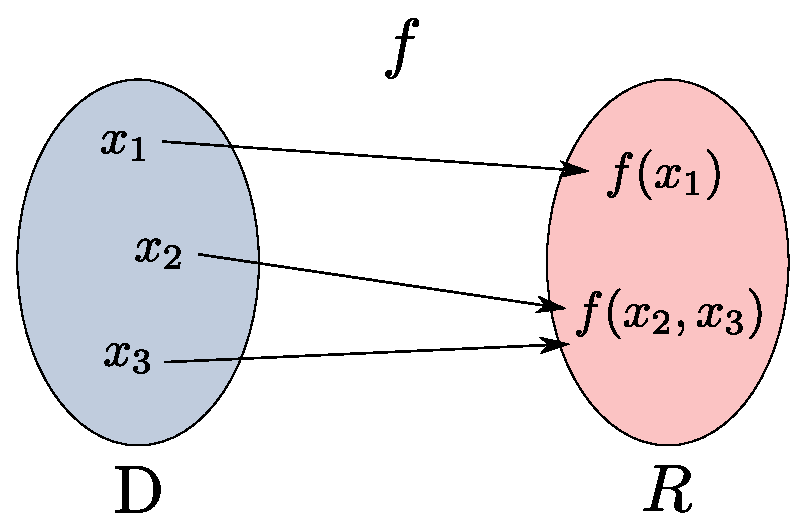
\includegraphics[width=0.4\textwidth]{continuous/functions/function.eps}
    \caption{A function $f$ mapping from $D$ to $R$. Note how multiple $x$ 
        values share the same $f(x)$ value.}
    \label{fig:function}
\end{figure}

One technique that can help us understand functions is by describing them with words,
including mathematical language.
We can discuss the behavior of a function in general,
describing its properties, or we can discuss its behavior in more specific terms,
like when we evaluate a function at a certain value.

We can also talk about functions using visual language, as in graphs, arrow 
diagrams, and tables.
% There are, of course, many ways to visually represent a function, but for our purposes these will prove the most useful.
% This includes some numerical displays of functions, like with a table of values.
% We can consider tables to be a visual description of a function because they combines visual formatting with descriptive data to produce a figural representation of a function's properties.

We will find graphs, in conjunction with the respective mathematical language, 
to be the most cohesive way to represent functions.
We should therefore attempt to be able to graph our functions whenever we wish to achieve the best possible understanding of them.

We will combine these techniques in an effort to paint a complete picture of its 
behavior.

\section{Properties of Functions}

Here, we will discuss a number of the properties that will be of interest when we
are describing functions.
Not all of these properties will exist for every type of function.
For example, not all functions will have an inverse 
(described in \secref{sec:inverse}), 
but the nonexistence of an inverse then becomes an important property of the 
function. % WHEN????? Tell the reader where this is useful.

\subsection{Domain and Range}

\begin{defn}
    The set $D$ of all possible input values is called the \textbf{domain} of 
    the function.
    \index{domain}
\end{defn}

\begin{defn}
    The set of all values $f(x)$ as $x$ varies throughout $D$ is called 
    the \textbf{range} of the function,
    representing the output value of $f$ at $x$.
    \index{range}
\end{defn}

\begin{defn}
    The \textbf{natural domain} of a function is the largest set of real 
    $x$-values for which a function returns real $y$-values.
    A function is said to be \textbf{real-valued} when $D = \mathbb{R}$.
\end{defn}
That is, the domain is equal to to the set of real numbers.
This means that we can put an arbitrary real number into the function and it 
will return a real $y$-value.

 \begin{remark}
     When we define a funciton $y=f(x)$ with a formula and the domain is not 
     stated explicitly or restricted by context, the domain is assumed to be the 
     \emph{natural domain}.
   \end{remark}
   \index{natural domain}

  The \textbf{vertical line test} for a function is based on the idea that if 
  $a$ is in the domain of the function $f$ then the vertical line $x=a$ will 
  intersect the graph of $f$ at a single point $ \big(a,f(a)\big)$.
  \index{vertical line test}

\begin{figure}[H]
  \begin{center}
    \subfigure[This passes the vertical line test]{\
      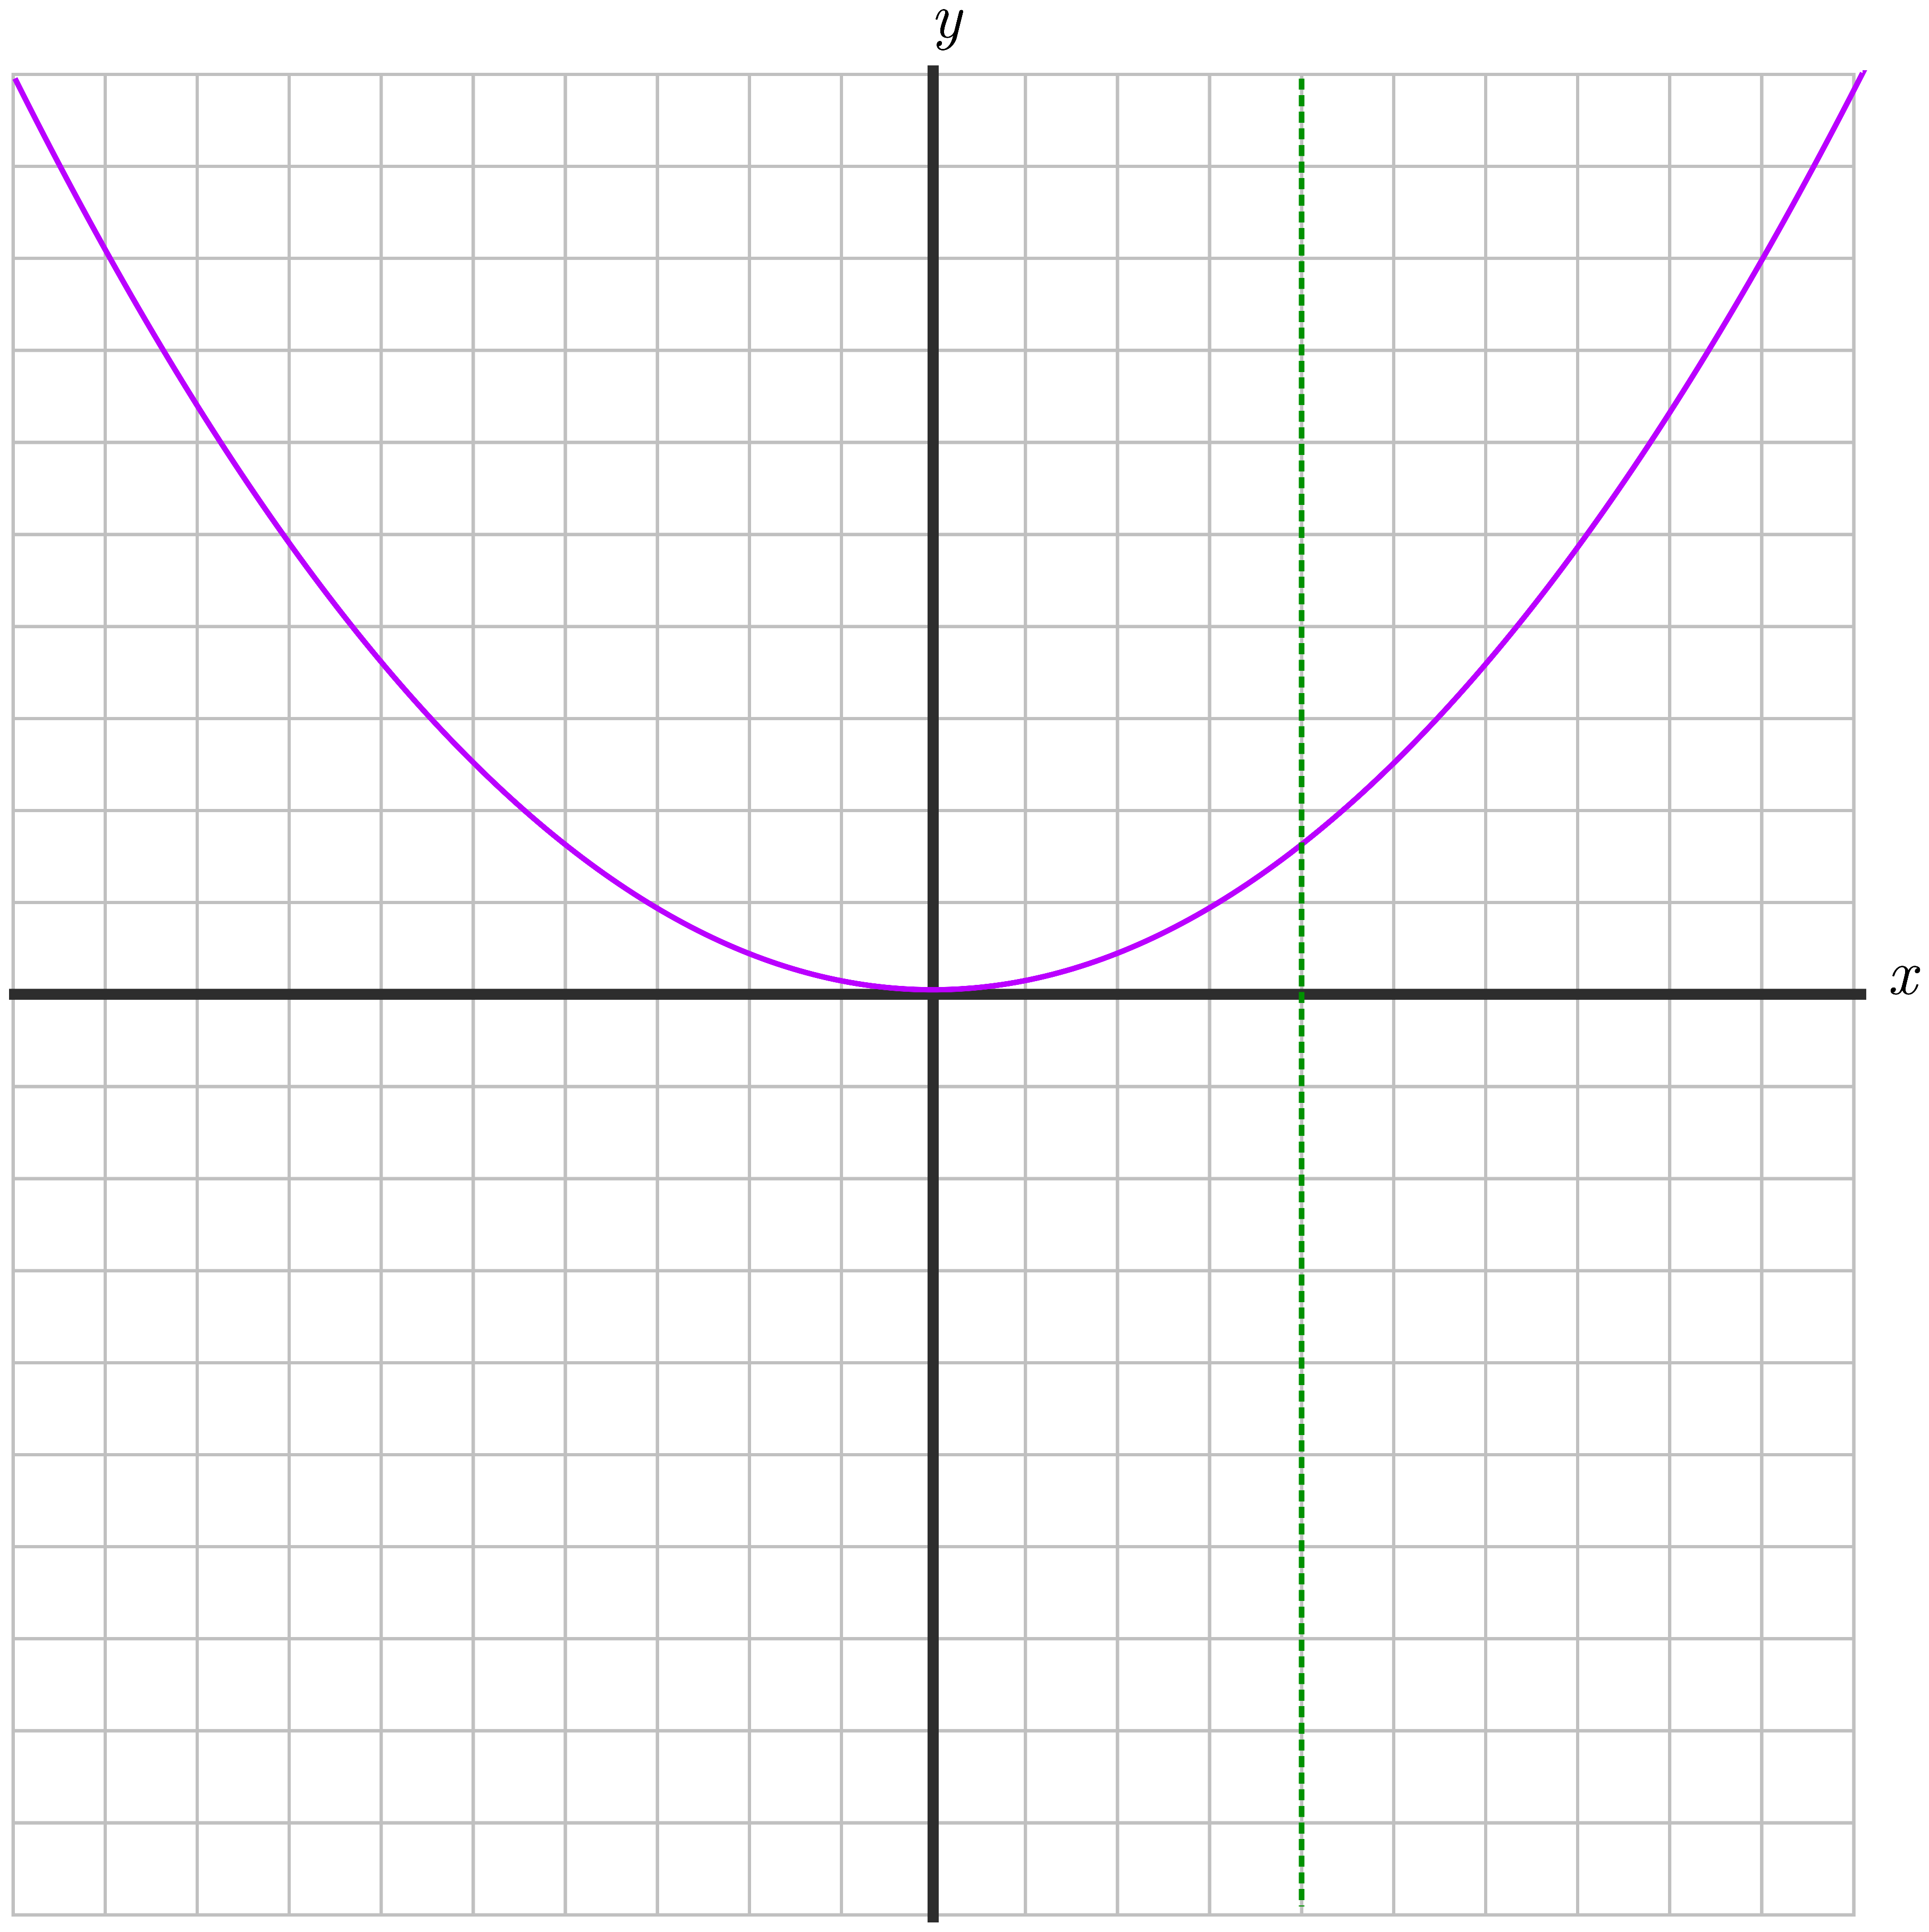
\includegraphics[width=0.4\textwidth]{continuous/functions/vlt1}
    }
    \subfigure[This fails the vertical line test]{\
      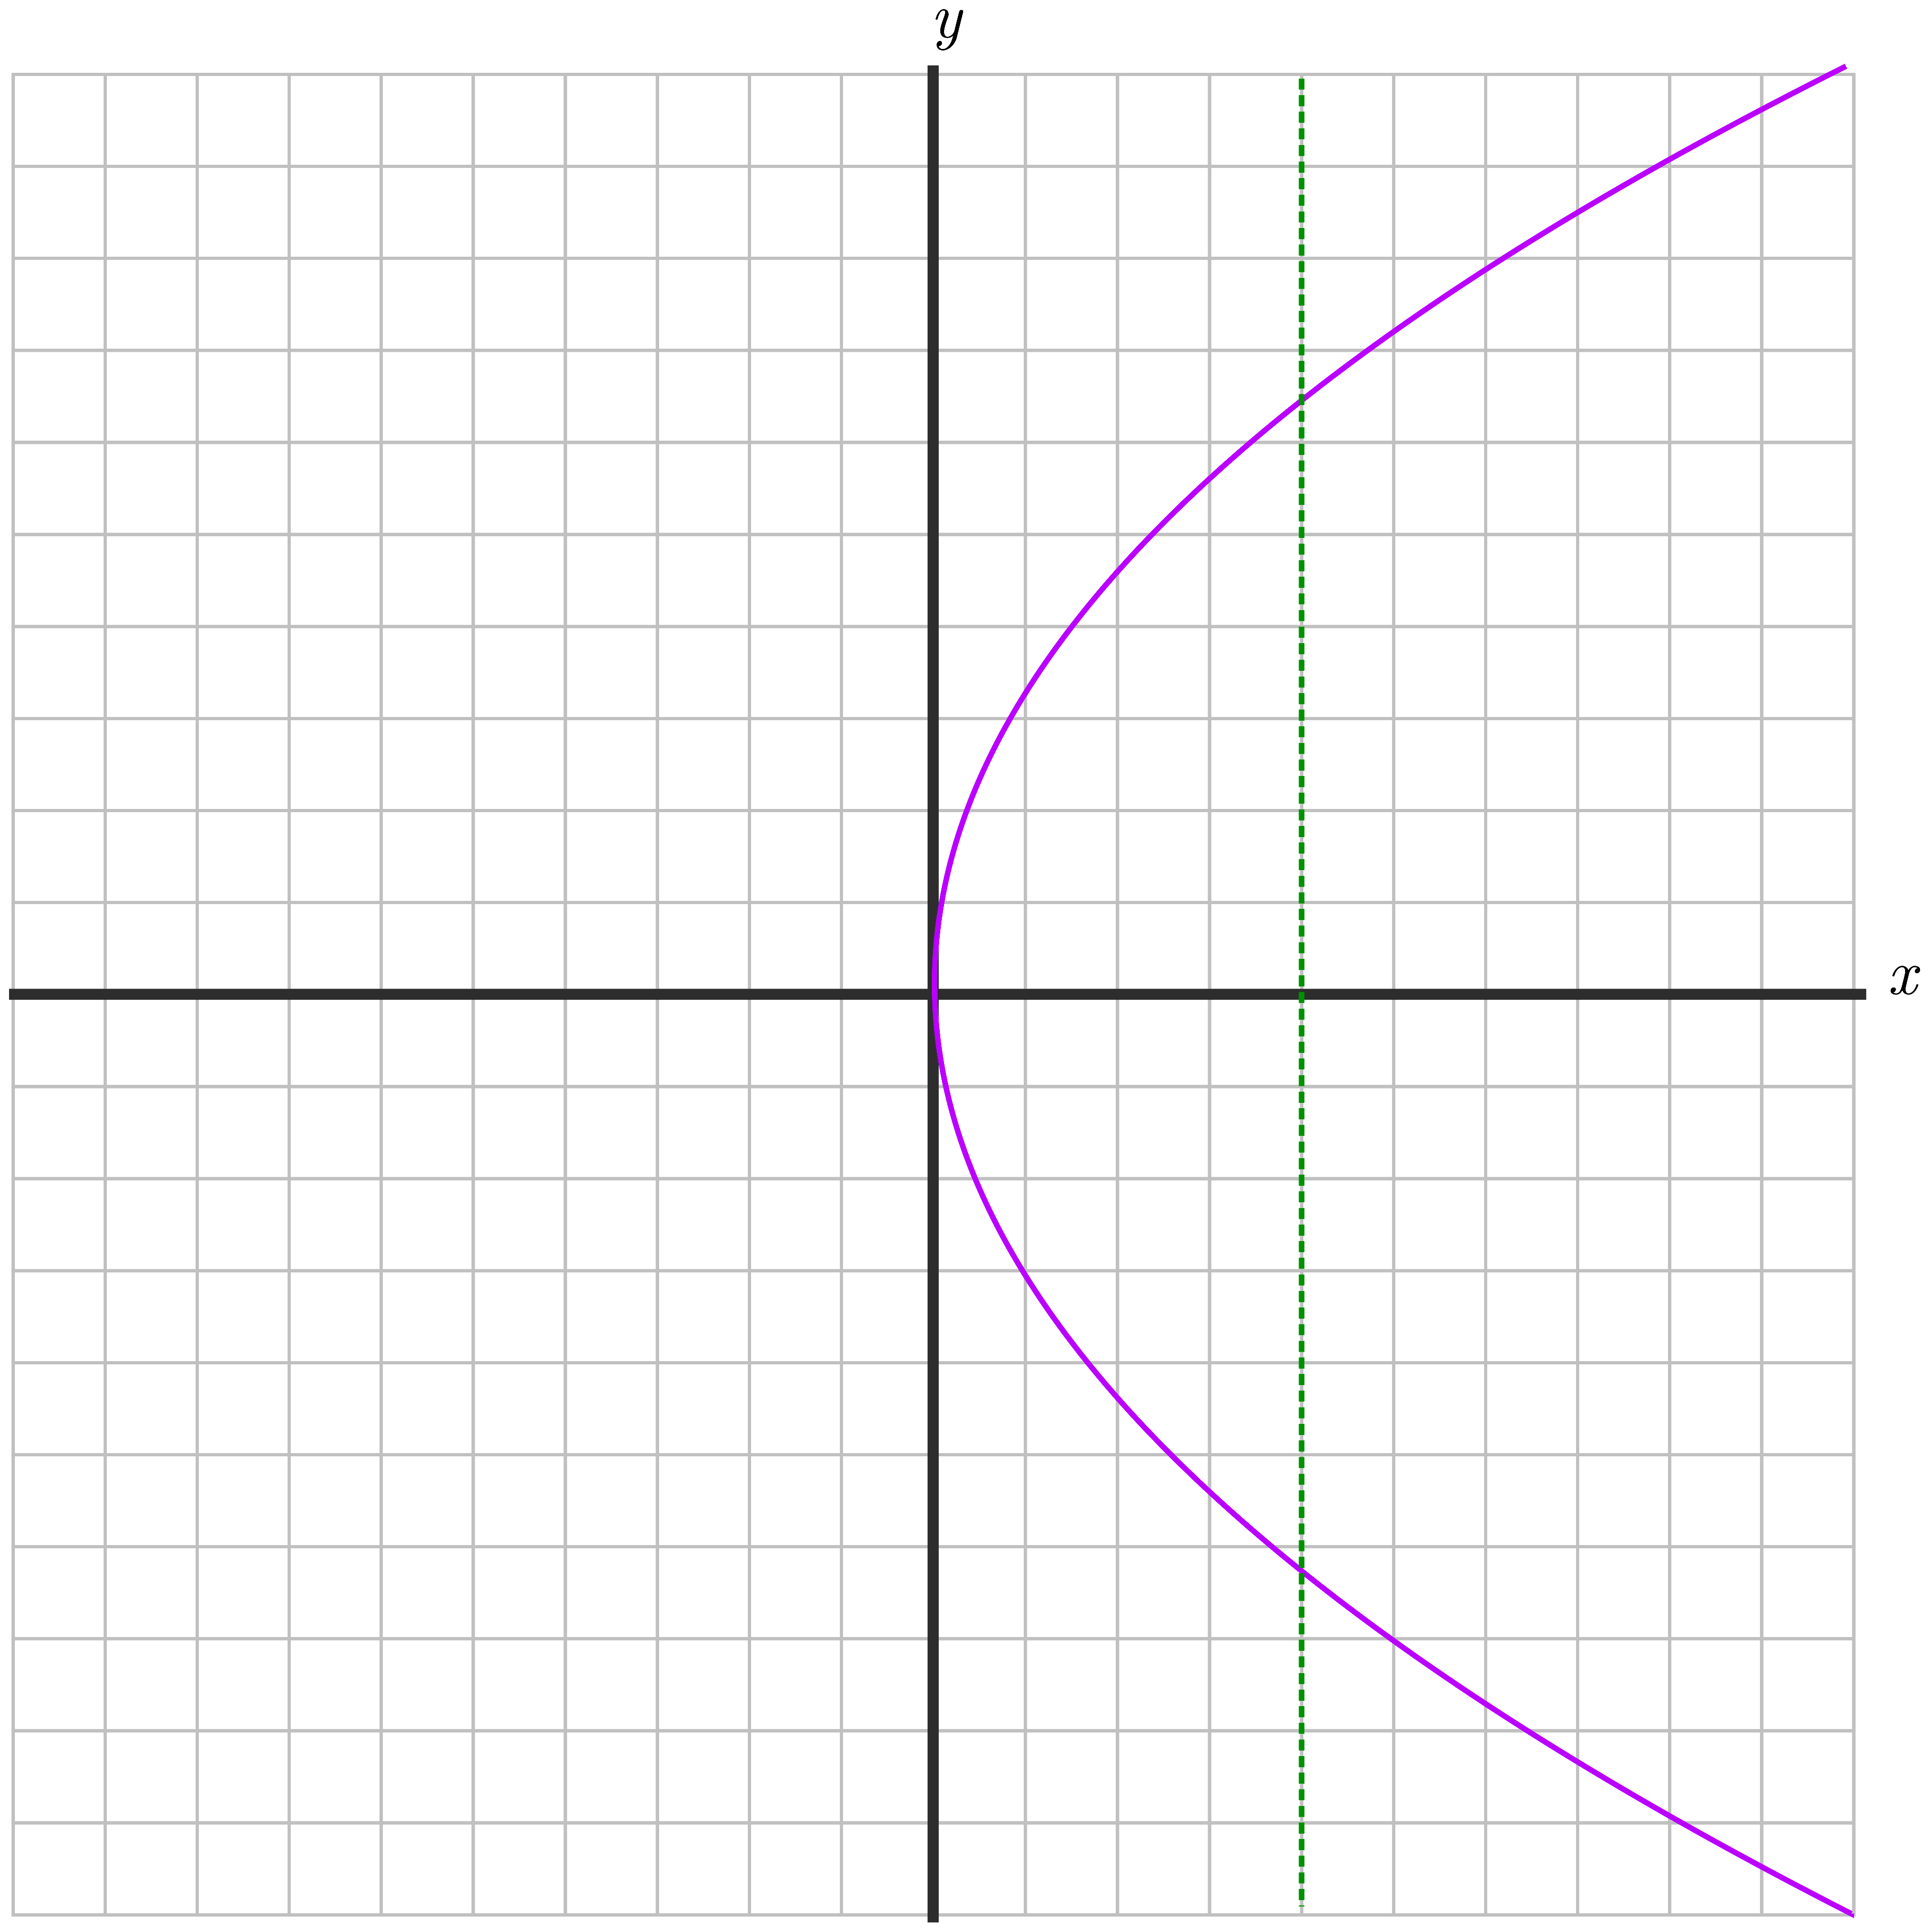
\includegraphics[width=0.4\textwidth]{continuous/functions/vlt2}
    }
  \end{center}
  \caption{Examples of the vertical line test.}
\end{figure}


\subsection{Dependent and Independent Variables}
  The letter $x$ in the notation $y=f(x)$ is called the 
  \textbf{independent variable} of the function, representing the input value 
  of $f$.
  \index{independent variable}

  The letter $y$ in the notation $y=f(x)$ is called the 
  \textbf{dependent variable}.
  It varies with respect to change in the dependent variable of the function.
  \index{dependent variable}

\subsection{Even and Odd Functions}

For a function $f$ in the form $y=f(x)$, we describe its type of symmetry by 
calling the function \textbf{even}\index{even functions} or 
\textbf{odd}\index{odd functions}.

An \textbf{even function} means $f(-x)=f(x)$.
An example of an even function is the function $f(x)=x^2$.
  \begin{figure}[H]
    \begin{center}
      \begin{tikzpicture}
        \begin{axis}[
            ylabel={$f(x)=x^2$},
            axis x line=bottom,
            axis y line=center,
            tick align=outside,
            yticklabels={,,}
            xticklabels={,,}
            xtickmax=10,
          ]
          \addplot[smooth,red]{x^2};
        \end{axis}
      \end{tikzpicture}
    \end{center}
    \caption{$f(x)=x^2$ is an \emph{even function}.}
  \end{figure}
  An \textbf{odd function} means $f(-x)=-f(x)$. An example of this is the 
  function $f(x)=x^3$.
  \begin{figure}[H]
    \begin{center}
      \begin{tikzpicture}
        \begin{axis}[
            ylabel={$f(x)=x^3$},
            axis x line=bottom,
            axis y line=center,
            tick align=outside,
            yticklabels={,,}
            xticklabels={,,}
            xtickmax=10,
          ]
          \addplot[smooth,red]{x^3};
        \end{axis}
      \end{tikzpicture}
    \end{center}
    \caption{$f(x)=x^3$ is an \emph{odd function}.}
  \end{figure}
\subsection{Surjective, Injective, and Bijective Functions}

\begin{defn}
  \index{one-to-one}
  \index{injective}
  If each $f(x)$ value produced by a function $f$ can only be obtained by one 
  unique $x$ value, then we say $f$ is \textbf{injective}, or 
  \textbf{one-to-one}.

  $ f: D \to R $ is injective or one-to-one iff
  \[
    \forall{(x_1 \wedge x_2 \in D)}
    \big[f(x_1)=f(x_2)
    \to x_1=x_2\big].
  \]
  \begin{remark}
    This also means that for injective functions,
    $ x_1 \neq x_2 \to f(x_1) \neq f(x_2)$.
  \end{remark}
\end{defn}
\begin{figure}[H]
    \begin{center}
        \subfigure[The function $f(x)=x^2$ is not \emph{one-to-one} because 
        there are two possible $x$-values that can produce each given 
        $y$-value.]
        {\
          \begin{tikzpicture}
            \begin{axis}[
                ylabel={$f(x)=x^2$},
                axis x line=bottom,
                axis y line=center,
                tick align=outside,
                yticklabels={,,}
                xticklabels={,,}
                xtickmax=10,
              ]
              \addplot[smooth,red]{x^2};
            \end{axis}
          \end{tikzpicture}
        }
        \hspace{0.2in}%
        \subfigure[The function $f(x)=x^3$ is \emph{one-to-one} because every 
        given $y$-value is mapped from a unique $x$-value.]
        {\
          \begin{tikzpicture}
            \begin{axis}[
                ylabel={$f(x)=x^3$},
                axis x line=bottom,
                axis y line=center,
                tick align=outside,
                yticklabels={,,}
                xticklabels={,,}
                xtickmax=10,
              ]
              \addplot[smooth,blue]{x^3};
            \end{axis}
          \end{tikzpicture}
        }
    \end{center}
  \end{figure}
  A function $y=f(x)$ is one-to-one iff its graph intersects each horizontal 
  line at most once.\index{horizontal line test}
\begin{defn}
  \index{onto}
  \index{surjective}
  $f: D \to R $ is \textbf{surjective} or \textbf{onto} iff
    \[\forall (y \in R) \exists  (x \in D) \big[f(x)=y\big]. \]
\end{defn}
\begin{figure}[H]
    \begin{center}
        \subfigure[The function $f(x)=x^2$ is not \emph{surjective} because 
        the values $(-\infty, 0)$ are never reached in its range.]
        {\
          \begin{tikzpicture}
            \begin{axis}[
                ylabel={$f(x)=x^2$},
                axis x line=bottom,
                axis y line=center,
                tick align=outside,
                yticklabels={,,}
                xticklabels={,,}
                xtickmax=10,
              ]
              \addplot[smooth,red]{x^2};
            \end{axis}
          \end{tikzpicture}
        }
        \hspace{0.2in}%
        \subfigure[The function $f(x)=x^3$ is \emph{one-to-one} because all $y$ values from $-\infty, \infty)$ have corresponding $x$-values.]
        {\
          \begin{tikzpicture}
            \begin{axis}[
                ylabel={$f(x)=x^3$},
                axis x line=bottom,
                axis y line=center,
                tick align=outside,
                yticklabels={,,}
                xticklabels={,,}
                xtickmax=10,
              ]
              \addplot[smooth,blue]{x^3};
            \end{axis}
          \end{tikzpicture}
        }
    \end{center}
  \end{figure}

  \begin{defn}
    \index{bijective}
    A function $f:A \to B$ is \textbf{bijective} iff it is \emph{both injective and surjective}.
  \end{defn}
\begin{figure}[H]
    \begin{center}
        \subfigure[The function $f(x)=x^2$ is not bijective.]
        {\
          \begin{tikzpicture}
            \begin{axis}[
                ylabel={$f(x)=x^2$},
                xlabel={$x$},
                axis x line=bottom,
                axis y line=center,
                tick align=outside,
                yticklabels={,,}
                xticklabels={,,}
                xtickmax=10,
              ]
              \addplot[smooth,red]{x^2};
            \end{axis}
          \end{tikzpicture}
        }
        \hspace{0.2in}%
        \subfigure[The function $f(x)=x^3$ is bijective.]
        {\
          \begin{tikzpicture}
            \begin{axis}[
                ylabel={$f(x)=x^3$},
                xlabel={$x$},
                axis x line=bottom,
                axis y line=center,
                tick align=outside,
                yticklabels={,,}
                xticklabels={,,}
                xtickmax=10,
              ]
              \addplot[smooth,blue]{x^3};
            \end{axis}
          \end{tikzpicture}
        }
    \end{center}
  \end{figure}


\subsection{Graphs} \index{graphs}

\begin{defn}
  \index{graph}
    If $f$ is a function with a domain $D$, then its \textbf{graph} is the set
    \[ \Big\{ \big( x,f(x) \big) \Big | x \in D \Big\},\]
    that is, it is the set of all points $(x, f(x))$ where $x$ is in the domain of the function.%
\footnote{Here, the difference between the words \emph{graph} and \emph{plot} is sometimes confusing. Technically speaking, a \emph{graph} is the set defined explicitly here, while a function's \emph{plot} refers to any pictorial representation of a data set. However, since the usage is inconsistent in this text, these formal definitions will usually not apply. It can be safely assumed that as long as we are within the realm of real numbers, all uses of either \emph{graph} or \emph{plot} hereafter simply refer to the pictorial representation of a function's graph in the form of a curve on the cartesian plane.}
\end{defn}

If $ (x,y) $ is a point on $f$, then $y=f(x)$ is the height of the graph above point $x$.
This height might be positive or negative, depending on the sign of $f(x)$.
We use this height relationship to plot functions.
\begin{figure}[H]
    \begin{center}
        \begin{tikzpicture}
          \begin{axis}[
              ylabel={$f(x)$},
              xlabel={$x$},
              axis x line=bottom,
              axis y line=center,
              tick align=outside,
              yticklabels={,,}
              xticklabels={,,}
              xtickmax=10,
            ]
            \addplot[smooth,red]{x+2};
          \end{axis}
        \end{tikzpicture}
      \caption{A plot of the function $f(x)=x+2$}
    \end{center}
  \end{figure}

\section{Composition of Functions}
\label{sec:compositefunctions}
\begin{defn}
  If $f$ and $g$ are functions, then the \textbf{composite} function 
  $f \circ g$, ``$f$ composed with $g$'', is defined by
  \[ (f \circ g)(x)=f\bigl(g(x)\bigr) \text{.} \]
  \begin{remark}
    The domain of $ f \circ g $ consists of the numbers $x$ in the domain of 
    $g$ for which $g(x)$ lies in the domain of $f$.
    See figure~\ref{fig:p1sin1x} for an example of a function which produces 
    indefinite $y$-values for real $x$-values around $x=0$.
  \end{remark}
  \index{composition}
\end{defn}
\begin{ex}
  If
  $f(x)=x^2$
  and
  $g(x)=1-\sqrt{x}$,
  find $ (f \circ g)(x) $ and $ (g \circ f)(x)$.
  \begin{sol}
      We know that $(f \circ g)(x)$ is just $f(g(x))$ so
      \[ f(g(x)) = (1 - \sqrt x )^2. \] For $(g \circ f)(x)$ it is the opposite
      and \[ g(f(x)) = 1 - \sqrt{x^2} ,\]
      which is equivalent to saying \[ g(f(x)) = 1 - \abs{x}. \]
  \end{sol}
\end{ex}

\section{Inverse Functions}\index{inverse functions}\label{sec:inverse}
An inverse function undoes, or inverts, the effects of an original function.
% Old gibberish from when this was in the transcendental section.
%While inverse functions are not, by definition, transcendental, we will look 
%at them in this chapter because they are useful for producing inverse 
%trigonometric functions--functions that are transcendental.
They are useful for producing inverse trigonometric functions--functions that 
are transcendental.

\begin{defn}
  Suppose that $f$ is a one-to-one function on a domain $D$ with range $R$. The 
  \textbf{inverse function} $f^{-1}$ is defined by
  \[ f^{-1}(b)=a \text{ if } f(a)=b. \]
  The domain of $f^{-1}$ is $R$ and the range of $f^{-1}$ is $D$.
  \index{inverse functions}
\end{defn}
In order for an inverse function $f^{-1}(x)$ to exist for a function $f(x)$, 
the original function $f(x)$ must be one-to-one. Otherwise, the resulting 
``inverse function'' would not be a function: more than one output would be 
produced from only one input, and it would not pass the vertical line test.
\begin{figure}[H]
  \begin{center}
    \subfigure[A plot of $f(x)=\sqrt x$.]{\
      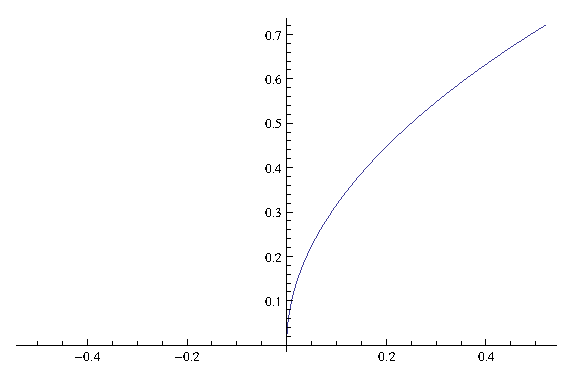
\includegraphics[width=0.3\textwidth]{continuous/functions/sqrtx}
    }
    \subfigure[A plot of $f^{-1}(\sqrt x)=x^2$.]{\
      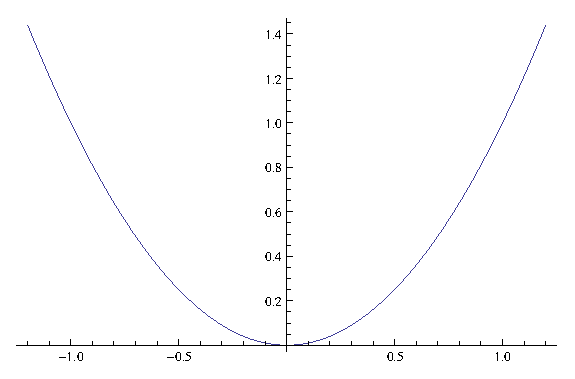
\includegraphics[width=0.3\textwidth]{continuous/functions/x2inv}
    }
  \end{center}
  \label{fig:inversef}
\end{figure}
\begin{remark} \index{composition}\index{inverse functions}
  By definition, either composite of a function and its inverse will return the 
  identity function, where $y=x$. For example:
  \[ (f \circ f^{-1})(x)=f(f^{-1}(x))=x, \]
  or
  \[ (f^{-1} \circ f)(x)=f^{-1}(f(x))=x. \]
\end{remark}

\subsection{Finding Inverse Functions}
To find the inverse of a function $f(x)$, replace $f(x)$ with $y$ and solve for 
$x$ in terms of $y$. Then, interchange $x$ and $y$.
\begin{ex}
  \label{ex:inverses}
  Find the inverse of $y=\frac{1}{2}x+1$, expressed as a function of $x$.
  \begin{sol}
    First, we solve the function for $x$ in terms of $y$.
    \begin{align*}
      y &= \frac{1}{2}x+1 \\
      \intertext{Multiply both sides by $2$.}
      2y &= x + 2 \\
      \intertext{Now subtract $2$ from both sides, and swap the left and right 
          sides of the equation.}
      x &= 2y -2
      \intertext{Now we swap $x$ and $y$.}
      y &=2x-2
    \end{align*}
    The inverse of the function $f(x)=\frac{1}{2}x+1$ is the function 
    $f^{-1}(x)=2x-2$.
    \begin{figure}[H]
      \begin{center}
        \subfigure[A plot of $f(x)=\frac{1}{2}x+1$.]{\
          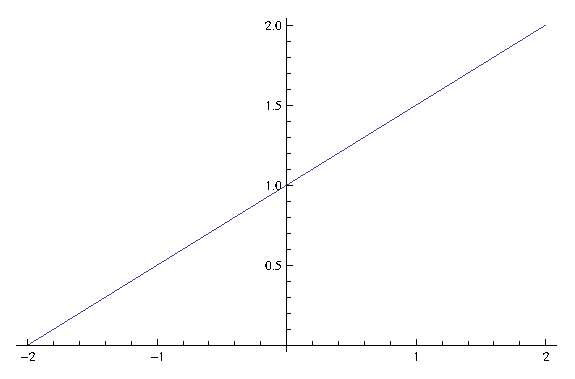
\includegraphics[width=0.45\textwidth]{continuous/functions/halfxeg}
        }
        \subfigure[A plot of $f^{-1}(x)=2x-2$.]{\
          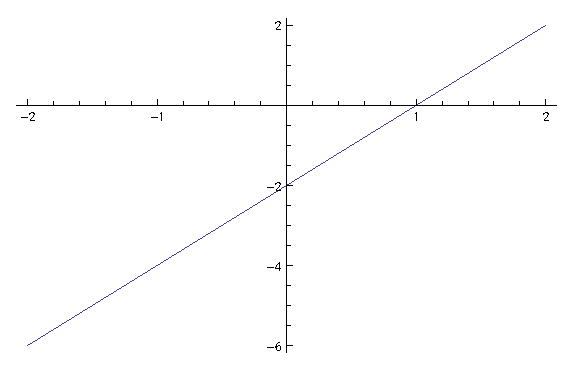
\includegraphics[width=0.45\textwidth]{continuous/functions/halfxeginv}
        }
      \end{center}
      \caption{Plots of functions from Example~\ref{ex:inverses}.}
      \label{fig:inverseg}
    \end{figure}
  \end{sol}
\end{ex}

\chapter{Trigonometry}


\section{Trigonometric Identities}\index{trigonometric identities}
\begin{figure}[h]
  \begin{center}
      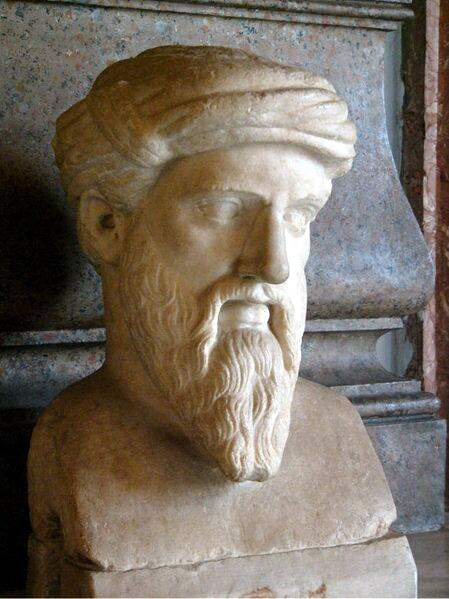
\includegraphics[width=0.7\textwidth]{photos/pythagoras.jpg}
    \end{center}
    \caption{/emph{Busto di Pitagora. Copia romana di originale greco. Musei Capitolini, Roma}.
    Original uploader was \emph{Galilea} at \url{http://de.wikipedia.org}.
    File used under the terms of the Creative Commons Attribution-Share Alike 3.0 Unported license.}
  \label{fig:bustofpythagoras}
\end{figure}
\begin{figure}[h]
  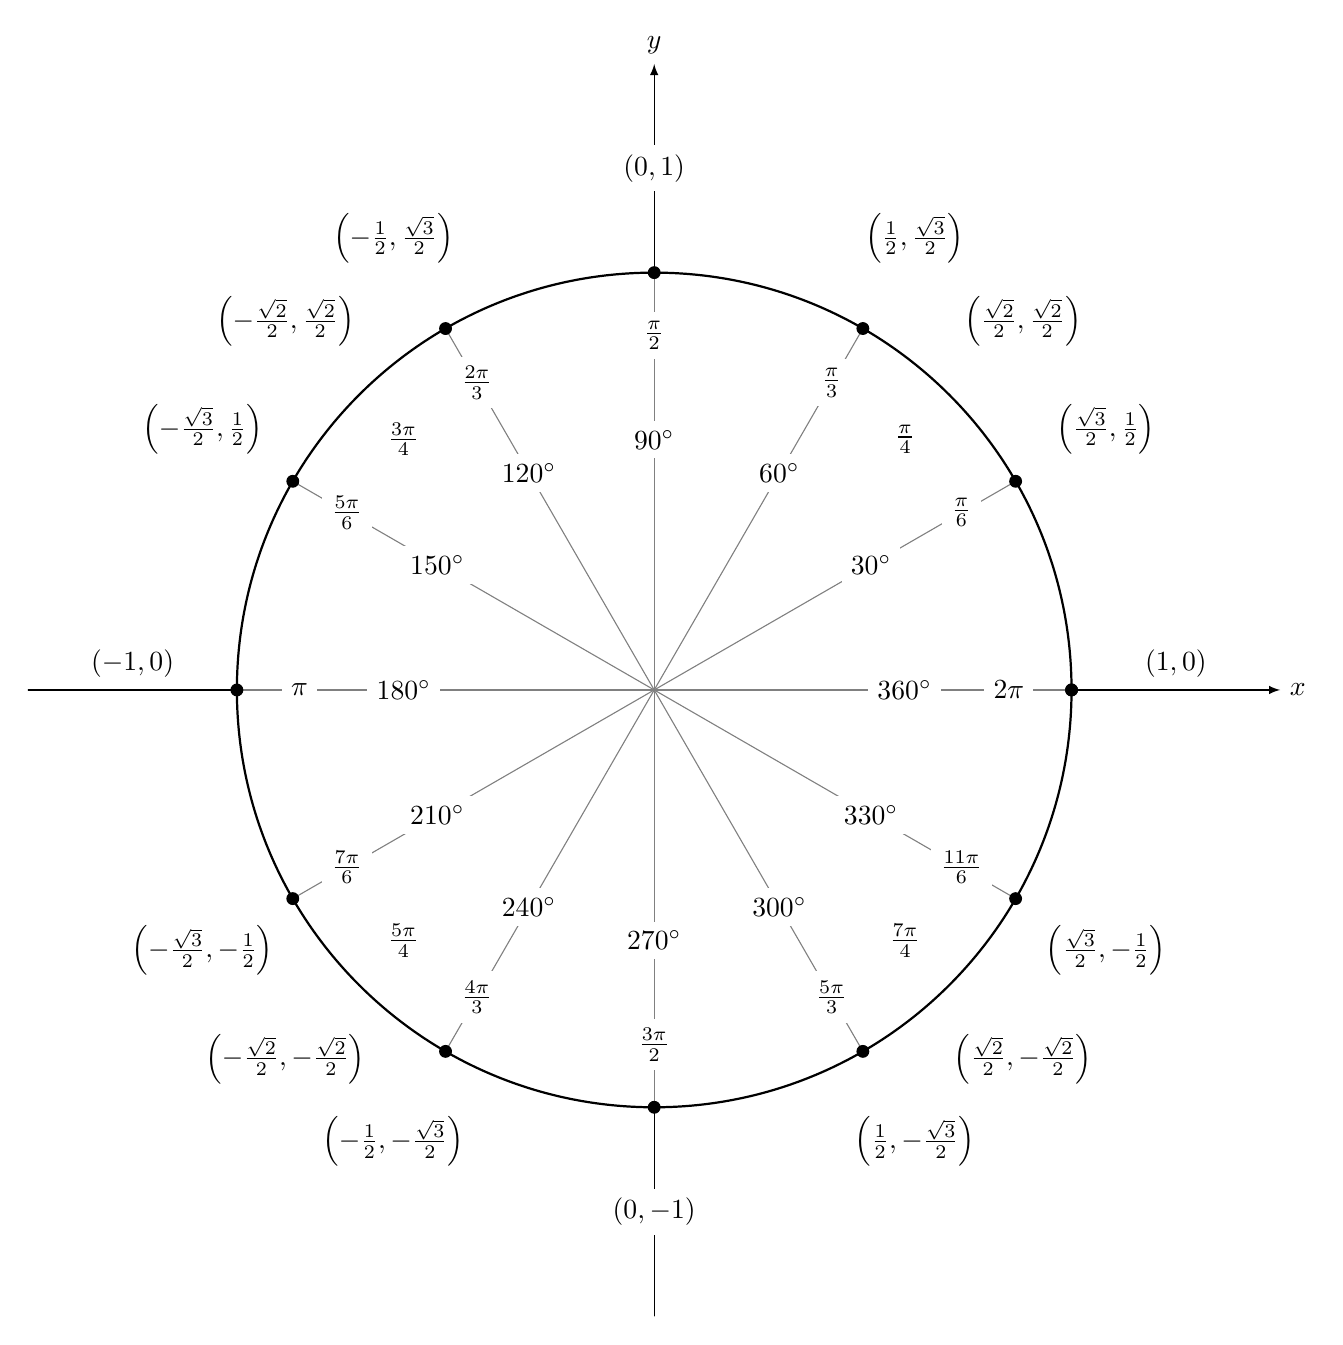
\begin{tikzpicture}[scale=5.3,cap=round,>=latex]
  % draw the coordinates
    \draw[->] (-1.5cm,0cm) -- (1.5cm,0cm) node[right,fill=white] {$x$};
    \draw[->] (0cm,-1.5cm) -- (0cm,1.5cm) node[above,fill=white] {$y$};

  % draw the unit circle
    \draw[thick] (0cm,0cm) circle(1cm);

    \foreach \x in {0,30,...,360} {
          % lines from center to point
      \draw[gray] (0cm,0cm) -- (\x:1cm);
          % dots at each point
      \filldraw[black] (\x:1cm) circle(0.4pt);
          % draw each angle in degrees
      \draw (\x:0.6cm) node[fill=white] {$\x^\circ$};
    }

  % draw each angle in radians
    \foreach \x/\xtext in {
      30/\frac{\pi}{6},
      45/\frac{\pi}{4},
      60/\frac{\pi}{3},
      90/\frac{\pi}{2},
      120/\frac{2\pi}{3},
      135/\frac{3\pi}{4},
      150/\frac{5\pi}{6},
      180/\pi,
      210/\frac{7\pi}{6},
      225/\frac{5\pi}{4},
      240/\frac{4\pi}{3},
      270/\frac{3\pi}{2},
      300/\frac{5\pi}{3},
      315/\frac{7\pi}{4},
      330/\frac{11\pi}{6},
    360/2\pi}
    \draw (\x:0.85cm) node[fill=white] {$\xtext$};

    \foreach \x/\xtext/\y in {
      % the coordinates for the first quadrant
      30/\frac{\sqrt{3}}{2}/\frac{1}{2},
      45/\frac{\sqrt{2}}{2}/\frac{\sqrt{2}}{2},
      60/\frac{1}{2}/\frac{\sqrt{3}}{2},
      % the coordinates for the second quadrant
      150/-\frac{\sqrt{3}}{2}/\frac{1}{2},
      135/-\frac{\sqrt{2}}{2}/\frac{\sqrt{2}}{2},
      120/-\frac{1}{2}/\frac{\sqrt{3}}{2},
      % the coordinate on s for the third quadrant
      210/-\frac{\sqrt{3}}{2}/-\frac{1}{2},
      225/-\frac{\sqrt{2}}{2}/-\frac{\sqrt{2}}{2},
      240/-\frac{1}{2}/-\frac{\sqrt{3}}{2},
      % the coordinates for the fourth quadrant
      330/\frac{\sqrt{3}}{2}/-\frac{1}{2},
      315/\frac{\sqrt{2}}{2}/-\frac{\sqrt{2}}{2},
      300/\frac{1}{2}/-\frac{\sqrt{3}}{2}}
      \draw (\x:1.25cm) node[fill=white] {$\left(\xtext,\y\right)$};

  % draw the horizontal and vertical coordinates
  % the placement is better this way
      \draw (-1.25cm,0cm) node[above=1pt] {$(-1,0)$}
      (1.25cm,0cm)  node[above=1pt] {$(1,0)$}
      (0cm,-1.25cm) node[fill=white] {$(0,-1)$}
      (0cm,1.25cm)  node[fill=white] {$(0,1)$};
  \end{tikzpicture}
  \caption{The unit circle.\cite{tikzunitcirc}\label{fig:tikzunitcirc}}
\end{figure}

Our first pythagorean identity is just derived from the pythagorean theorem.
\begin{figure}[H]
  \begin{center}
    \subfigure[The Pythagorean Theorem states that the sum of the areas square $a$ and square $b$ is equal to the area of square $c$.]{
      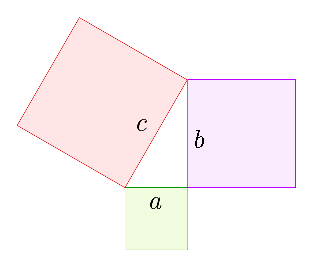
\includegraphics{continuous/functions/pyth.eps}
      \label{fig:pyth}
    }
    \hspace{0.1\textwidth}
    \subfigure[The equation for a unit circle is $a^2+b^2=1$. This creates a circle with a radius of $1$.]{
      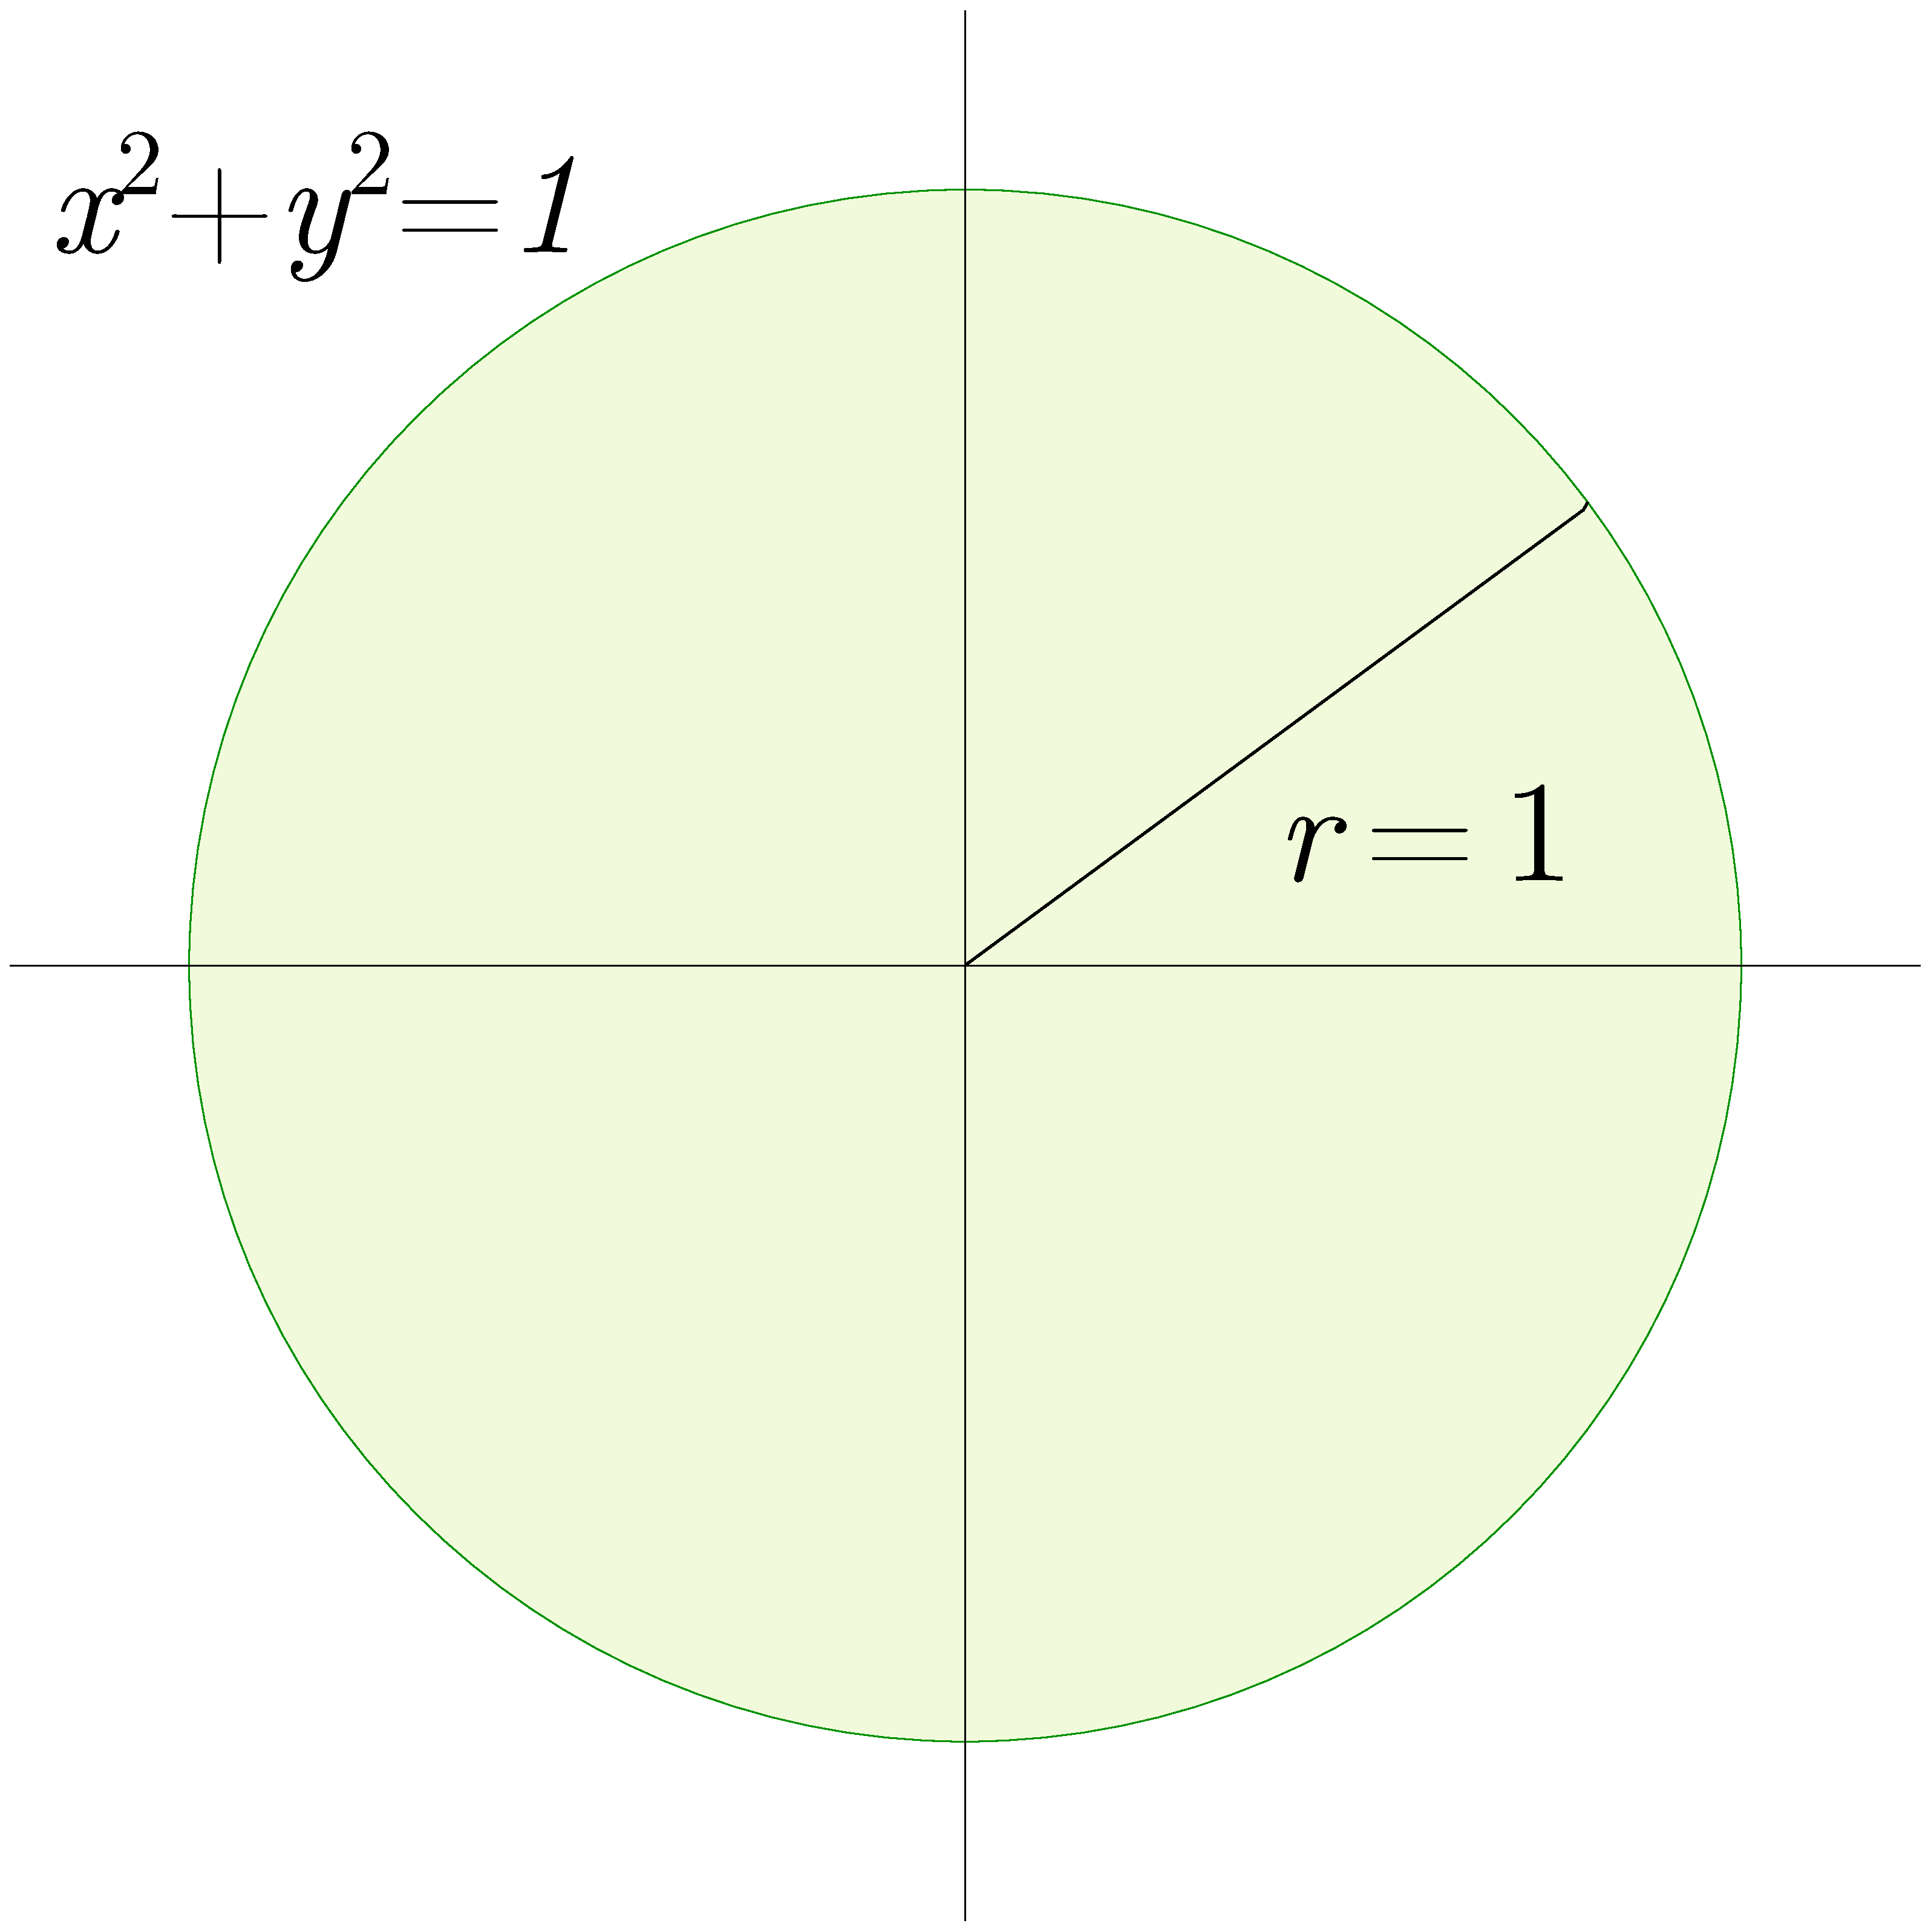
\includegraphics[width=0.3\textwidth]{continuous/functions/unitcirc.eps}
      \label{fig:basicuniticircle}
    }
  \end{center}
\end{figure}
\begin{equation}
  \sin^2x+\cos^2x=1
  \label{eq:pythtrig}
\end{equation}
\begin{figure}[H]
  \begin{center}
    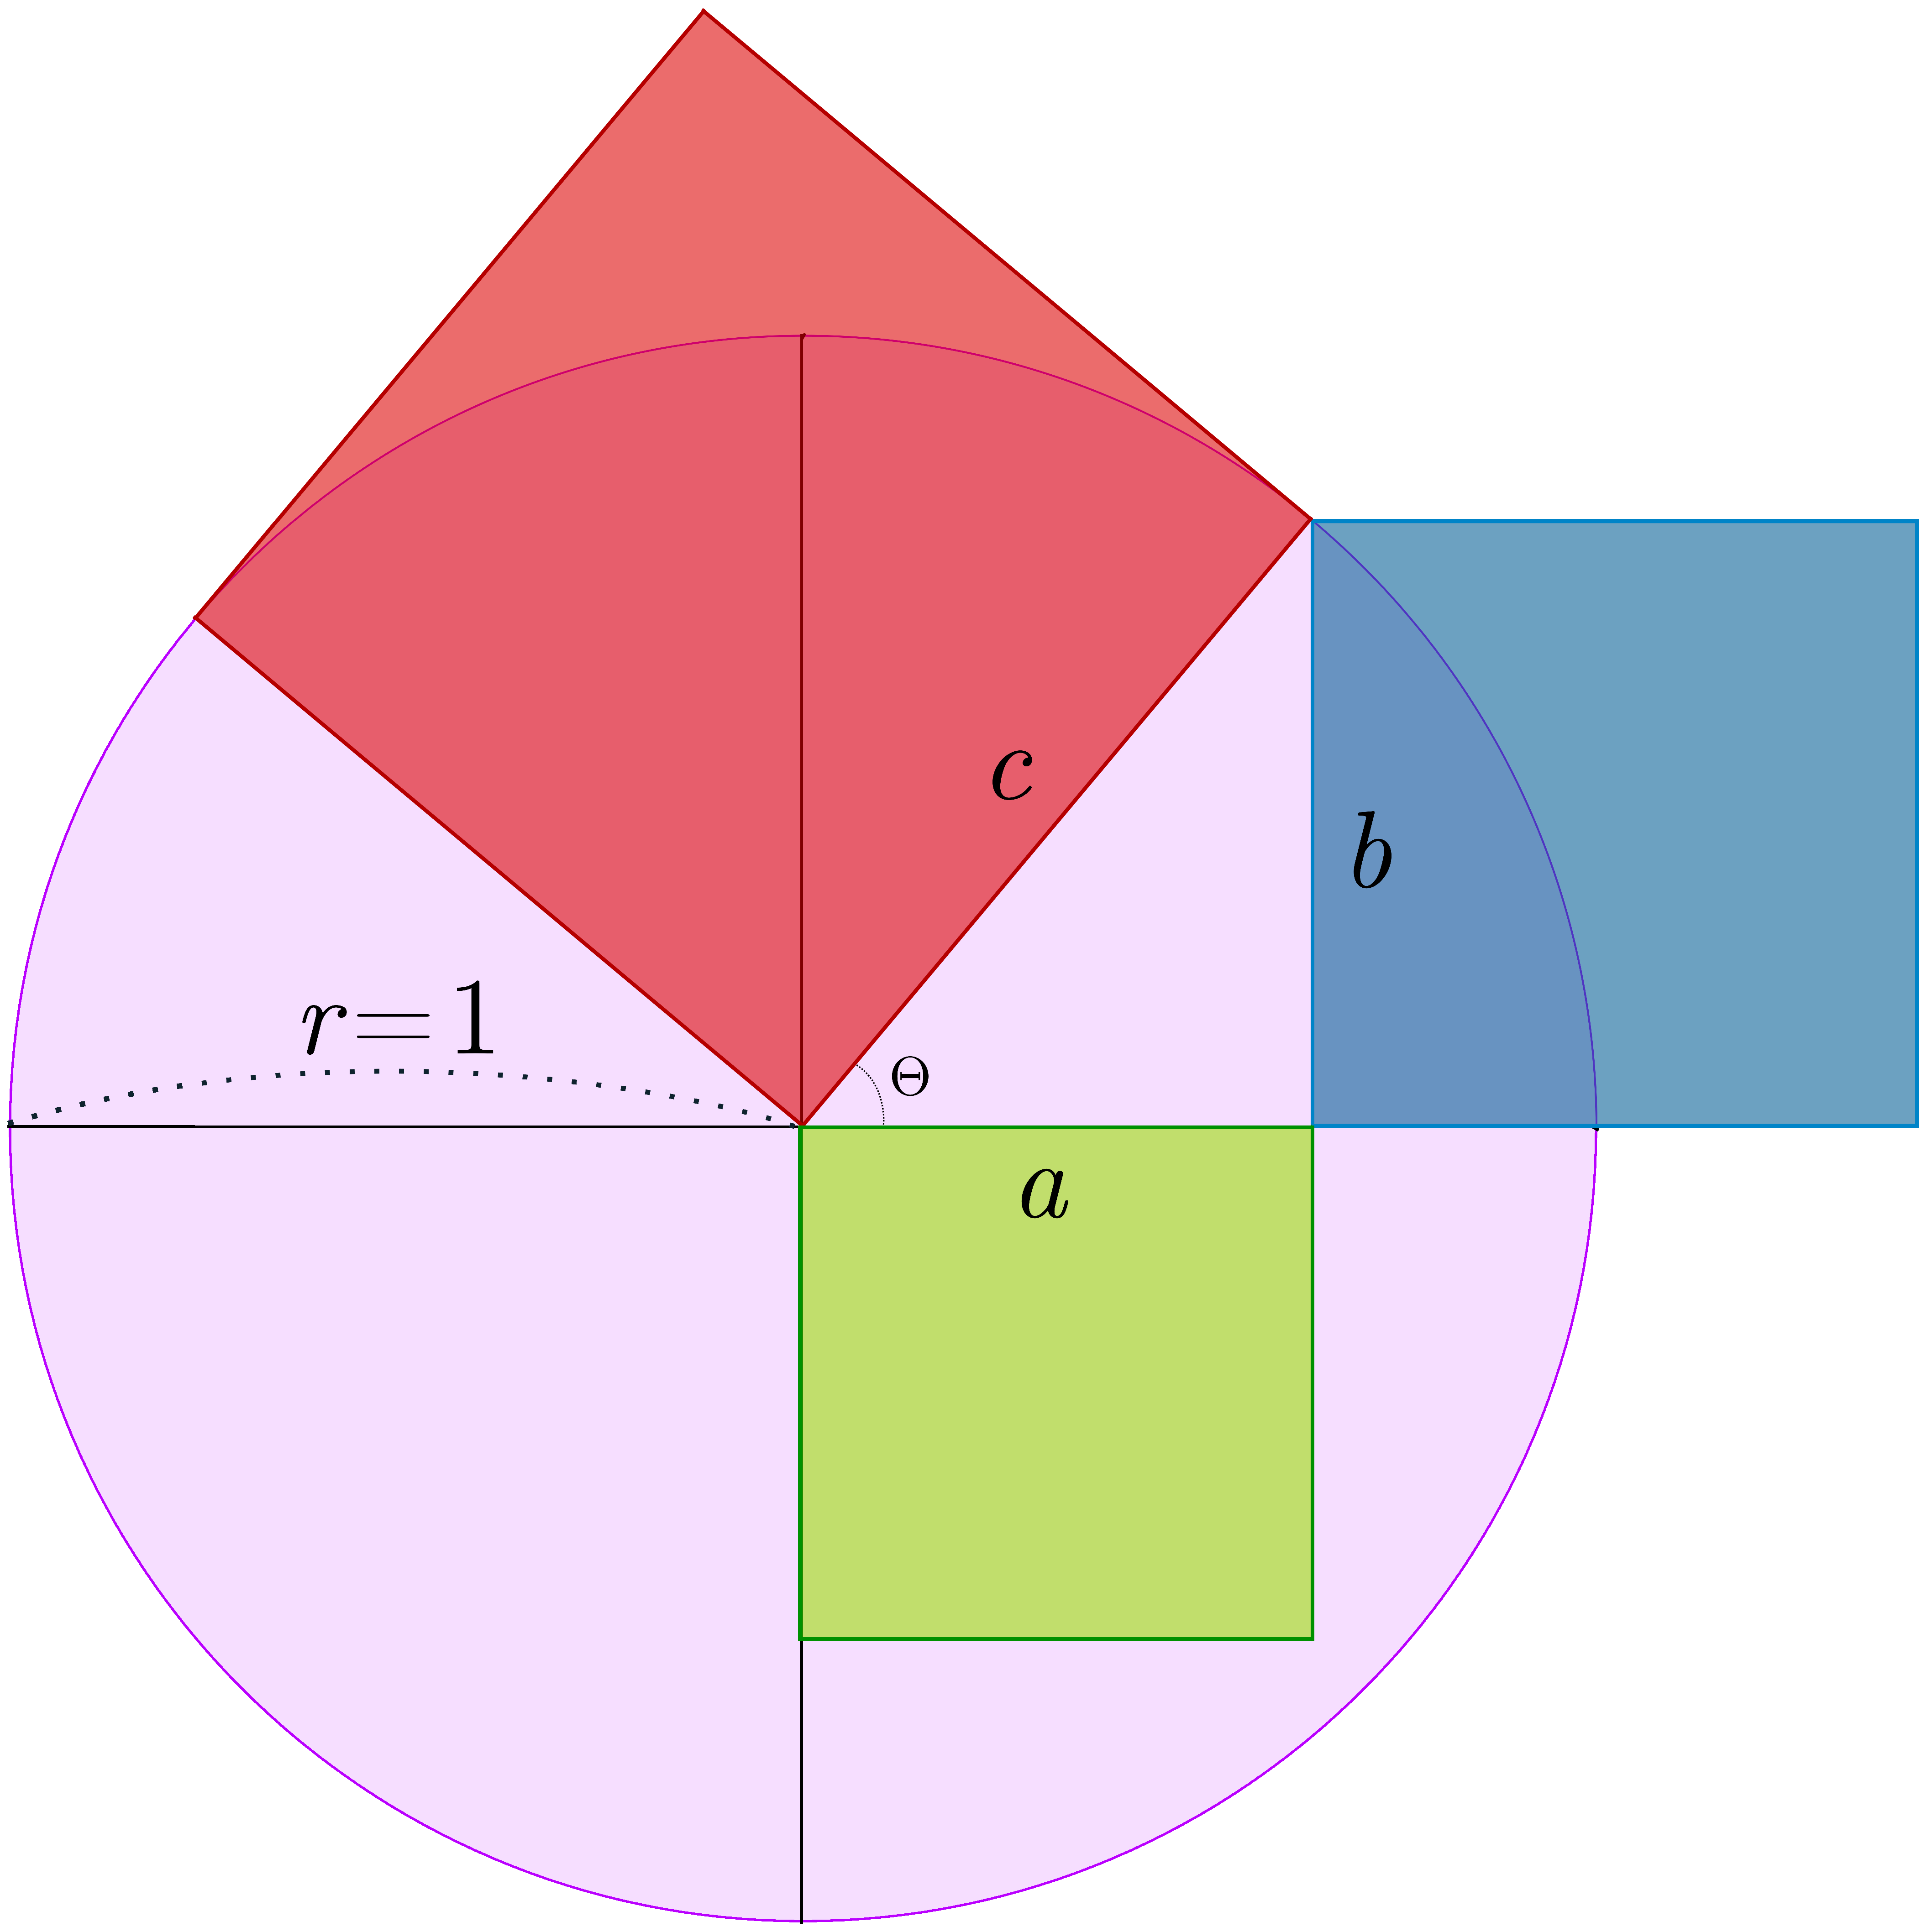
\includegraphics[width=0.3\textwidth]{continuous/trig/pythcircle.eps}
    \caption{The pythagorean squares on a unit circle.}
  \end{center}
  \label{fig:pythcircle}
\end{figure}
Because the radius of the circle is $1$, then the length of side $c$ must also equal $1$.
From this, we can conclude that $\sin^2x+\cos^2x$ must, indeed, equal 1.

To make sure we understand this on a geometric level, let's first go over the basic trigonometric functions and their relationship with our triangle.
\begin{figure}[H]
  \begin{center}
    
\includegraphics[width=0.3\textwidth]{continuous/trig/basictrig.eps}
  \end{center}
\end{figure}
For this example:
\begin{itemize}
  \item $\sin\theta=b/c$
  \item $\cos\theta=a/c$
  \item $\tan\theta=b/a$
\end{itemize}
Gennerally speaking, for an angle $\theta$ on the inside of a triangle,
\begin{itemize}
  \item$\sin\theta$ is equal to the \emph{length of the opposite side divided by the length of the hypotenuse}.
  \item$\cos\theta$ is equal to the \emph{adjacent side divided by the hypotenuse}.
  \item$\tan\theta$ is equal to the \emph{opposite over the adjacent side}.
\end{itemize}

The other ones, we either have to memorize or learn to derive (described in Section \ref{sec:trigderiv}).
\begin{equation}
  \sin{(x+y)} = \sin x \cos y + \sin y \cos x
\end{equation}
\begin{equation}
  \sin{(x-y)} = \sin x \cos y - \sin y \cos x
\end{equation}
\begin{equation}
  \cos(x+y)=\cos x \cos y - \sin x \sin y
  \label{eq:cosxpy}
\end{equation}
\begin{equation}
  \cos(x-y)=\cos x \cos y + \sin x \sin y
\end{equation}
\begin{equation}
  \sin{-x}=-\sin x
\end{equation}
\begin{equation}
  \sin{-x}=-\sin x
\end{equation}
\begin{equation}
  \sin{2x}=2 \big( \sin x \cos x \big)
\end{equation}
\begin{equation}
  \cos{2x}=\cos^2x-\sin^2x
\end{equation}

\subsection{Deriving Trigonometric Identities}\index{deriving trigonometric identities}\label{sec:trigderiv}

Using the pythagorean theorem and a triangle with a hypotenuse of length $1$, we can obtain our first trigonometric identity:
\begin{equation}
	\sin^2x+\cos^2x=1
  \label{eq:pyth}
\end{equation}
Dividing by $\sin^2x$ gives us:
\begin{align}
\frac{\sin^2x}{\sin^2x}+\frac{\cos^2x}{\sin^2x}&=\frac{1}{\sin^2x} \nonumber \\
	1+\cot^2x&=\csc^2x
\end{align}
Dividing by $\cos^2x$ produces:
\begin{align}
  \frac{\sin^2x}{\cos^2x}+\frac{\cos^2x}{\cos^2x}+=&\frac{1}{\cos^2x} \nonumber \\
	\tan^2x+1=&\sec^2x
\end{align}

We should also memorize the following two identities:
\begin{equation}
  \sin{a+b}=\sin a \cos a + \sin b \cos b
  \label{eq:sinab}
\end{equation}
\begin{equation}
  \cos{a+b}=\cos a \cos b + \sin a \sin b
  \label{eq:cosab}
\end{equation}
From equation \eqref{eq:sinab} we can infer that
\begin{equation}
  \sin{2\theta}=2 \sin \theta \cos \theta
  \label{eq:sin2q}
\end{equation}
and from equation \eqref{eq:cosab} we can infer that
\begin{equation}
  \cos{2\theta}=\cos^2 \theta - \sin^2\theta
  \label{eq:cos2q}
\end{equation}

By rearranging \eqref{eq:cos2q} and substituting from \eqref{eq:pyth} we can derive power reduction identities for $\cos^2 \theta$
\begin{align}
  \cos{2\theta} &= \cos^2 \theta - \sin^2\theta \nonumber \\
  \cos{2\theta} + \sin^2\theta &= \cos^2\theta \nonumber \\
  \cos{2\theta} + (1-\cos^2 \theta) &=\cos^2\theta \nonumber \\
  \cos{2\theta} + 1 &= \cos^2\theta + \cos^2\theta \nonumber \\
  \cos{2\theta}+1 &= 2 \cos^2\theta \nonumber \\
  \cos^2\theta &= \frac{\cos{2\theta}+1}{2}
  \label{eq:cossqq}
\end{align}
and for $\sin^2 \theta$
\begin{align}
  \cos{2\theta} &= \cos^2 \theta - \sin^2\theta \nonumber \\
  \sin^2 \theta &= \cos^2 \theta - \cos{2 \theta} \nonumber \\
  \sin^2 \theta &= (1-\sin^2 \theta) - \cos{2 \theta} \nonumber \\
  2 \sin^2 \theta &= 1-\cos{2\theta} \nonumber \\
  \sin^2 \theta &= \frac{1-\cos{2\theta}}{2}
  \label{eq:sinsqq}
\end{align}


\subsection{Examples}

\begin{ex}
  Find the value of
  \[ \cos{\frac{11 \pi}{12}} \text{.}\]
  \begin{sol}
    We first rewrite the problem to fit one of our trigonometric identities,
    then use equation \eqref{eq:cosxpy} to break apart \(\cos{\frac{11 \pi}{12}}\).
    \begin{align*}
      \cos{\frac{11 \pi}{12}}
      =&\cos{\frac{\pi}{4}+\frac{2 \pi}{3}}
      =\cos{\frac{\pi}{4}} \cos{\frac{2\pi}{3}}
        -\sin\frac{\pi}{4} \sin\frac{2\pi}{3} \\
      \intertext{Unlike in the original problem, we can easily simplify our new expression.}
      \cos{\frac{\pi}{4}} \cos{\frac{2\pi}{3}}
        - \sin{\frac{\pi}{4}} \sin{\frac{2\pi}{3}}
      =& \frac{\sqrt 2}{2} \frac{-1}{2}
        -\frac{\sqrt 2}{2} \frac{\sqrt 3}{2}
      =\frac{-\sqrt 2}{4}
        - \frac{\sqrt{6}}{4} \\
      = &\frac{-\sqrt 2}{4}(1+\sqrt 3)
    \end{align*}
  \end{sol}
\end{ex}
\begin{ex}
  Prove the following trigonometric identity:
  \[ \frac{1-\cos x}{\sin x}=\frac{\sin x}{1+\cos x} \]
  \begin{proof}
    We first cross-multiply:
    \begin{align*}
      \ (1-\cos x)(1+\cos x) &= sin^2 x \\
      \intertext{then, using equation \eqref{eq:pythtrig}, we realize that we can replace \(\sin^2 x\) with \(1-\cos^2 x\).}
       (1-\cos x)(1+\cos x) &= 1-\cos^2x\\
      \intertext{Now we simplify.}
      1-\cos x + \cos x -\cos^2 &= 1-\cos^2x \\
      1-\cos^2x &= 1-\cos^2x \qedhere
    \end{align*}
  \end{proof}
\end{ex}



\chapter{Limits}\label{limits} \index{limits}
\section{Understanding Limits}
If we have a function \(f\), defined such that
\begin{equation}
  f(x)=\frac{x^2-1}{x-1} \qquad (x \neq 1)
  \label{eq:firstlimit}
\end{equation}
this function is not defined at \(x=1\), so we cannot directly discuss its behavior at \(x=1\).
\begin{figure}[h]
  \begin{center}
    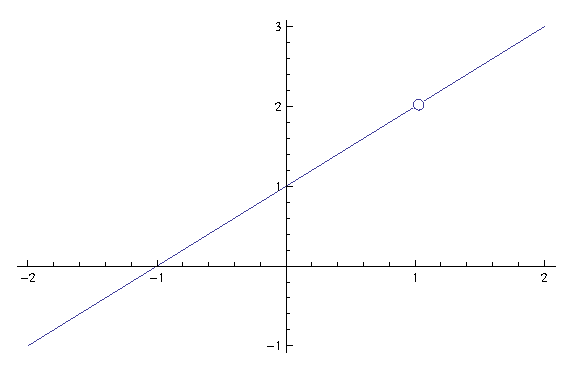
\includegraphics[scale=0.7]{graphs/p1ch3x2m1xm1}
  \end{center}
  \caption{A plot of \(f\). Note the hole at \(x=1\).}
\end{figure}
However, we may still wish to know how the function behaves \emph{around} \(x=1\).
This is where limits come in handy.
They discuss the behavior of a function near a specific point, without any consideration for how the function behaves exactly \emph{at} that point.
To find the behavior of \(f\) around \(x=1\), we take the limit of \(f\) as \(x\) approaches \(1\).
\begin{defn}\label{defn:limi}\index{limit definition}
  \( \lim_{x \to a} f(x) = L \) if and only if \(f(x)\) gets \emph{arbitrarily} close to \( L \) as \(x\) gets \emph{sufficiently} close to \(a\).
\end{defn}
\begin{remark}
  In this case, \textbf{arbitrarily close} implies that we can make the number as close as we could possibly request it. \textbf{sufficiently close} means that we can find a number $x$ where, for every number after (or before) it, we are past our arbitrary value of closeness.
\end{remark}
We would write this as:
\[ \lim_{x \to 1} \frac{x^2-1}{x-1} \]
In this case, we can evaluate this using basic algebra to simplify the original function,
\begin{align*}
   f(x)&=\frac{x^2-1}{x-1} && x \neq 1 \\
   &=\frac{(x+1)(x-1)}{x-1}&& x \neq 1 \\
   &=x+1 && x \neq 1
\end{align*}
\begin{remark}
  We must make the statement that $x \neq 1$ whenever $x+1$ is in the denominator of a function,
  because if $x$ could ever be equal to $1$, it would make the value of $f(x)$ undefined at this point.
\end{remark}
Then we define a new function equivalent to the above, but where \(1 \in D\).
We then evaluate our new function at \(x=1\).
\[ g(x) = x+1 \]
Which gives us
\begin{align*}
  \lim_{x \to 1} \frac{x^2-1}{x-1}
  &=g(1)
  \\&=2
  \text{.}
\end{align*}

It turns out we have a number of rules that describe how we can go about
evaluating a limit.
\begin{theorem}[Limit Laws]
  If \(L\), \(M\), and \(k\) are real numbers and
    \[ \lim_{x \to c} f(x)=L \quad and \lim_{x \to c} g(x) = M \]
  then,
  \begin{table}[H]
    \centering
      \begin{tabular}{p{3in}>\(p{3in}<\)}
        Sum Rule: & \displaystyle{\lim_{x \to c} (f(x) + g(x)) = L + M} \\ \\
        Difference Rule: & \displaystyle{\lim_{x \to c} (f(x) - g(x))=L-M} \\ \\
        Constant Multiple Rule: & \displaystyle{\lim_{x \to c} (k \cdot f(x)) = k
      \cdot L} \\ \\
      Quotient Rule: & \displaystyle{\lim_{x \to c} \frac{f(x)}{g(x)} =
      \frac{L}{M}, \quad m\neq 0} \\ \\
      Power Rule: & \displaystyle{\lim_{x \to c} [f(x)]^n = L^n, \quad n \in
      \mathbf{Z_+}} \\ \\
      Root Rule: & \displaystyle{\lim_{x \to c} \sqrt[n]{f(x)} =
      \sqrt[n]{L}=L^{1/n}, \quad n
    \in Z_+}
  \end{tabular}
  \end{table}
  If \(n\) is even, we assume that \(\lim_{x \to c} f(x) = L > 0\). This is because for the rules including exponents, for $\lim{x\to c} f(x)=L<0$ to be true we would require imaginary numbers.
\end{theorem}

Not all functions have limits defined everywhere on their domain.
For example, \(h(x)=\sin \frac{1}{x} \) oscillates indefinitely as \(x \to 0\), as shown in Figure \ref{fig:p1sin1x}.
\begin{figure}[H]
  \begin{center}
    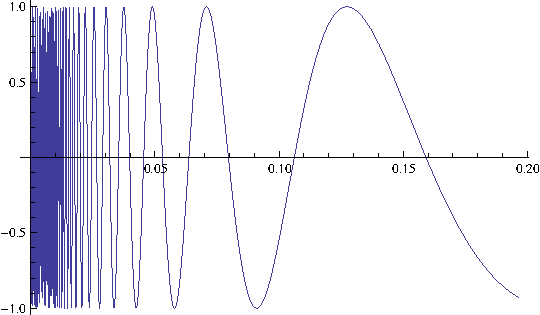
\includegraphics{graphs/p1sin1x.pdf}
  \end{center}
  \caption{The limit of \(h(x)\) as \(x \to 0\) does not exist.}
  \label{fig:p1sin1x}
\end{figure}
As \(x\to0\), it is impossible to say whether \(f(x)\) is approaching \(1\) or \(-1\).
This is an example of an \textbf{oscillating discontinuity}\index{oscillating discontinuity}.
There are more situations in which a limit does not exist.

In a \textbf{infinite discontinuity}\index{infinite discontinuity}, the graph jumps to $\infty$ or $-\infty$ at certain $x-values$.
No limit can exist here.
\begin{figure}[H]
  \begin{center}
    
\includegraphics[width=0.4\textwidth]{continuous/limits/infinited}
  \end{center}
  \caption{An infinite discontinuity at $x=0$.}
\end{figure}

The other situation which can cause a limit to not exist at a point is a \textbf{jump discontinuity}\index{jump discontinuity}.
\begin{figure}[H]
  \begin{center}
    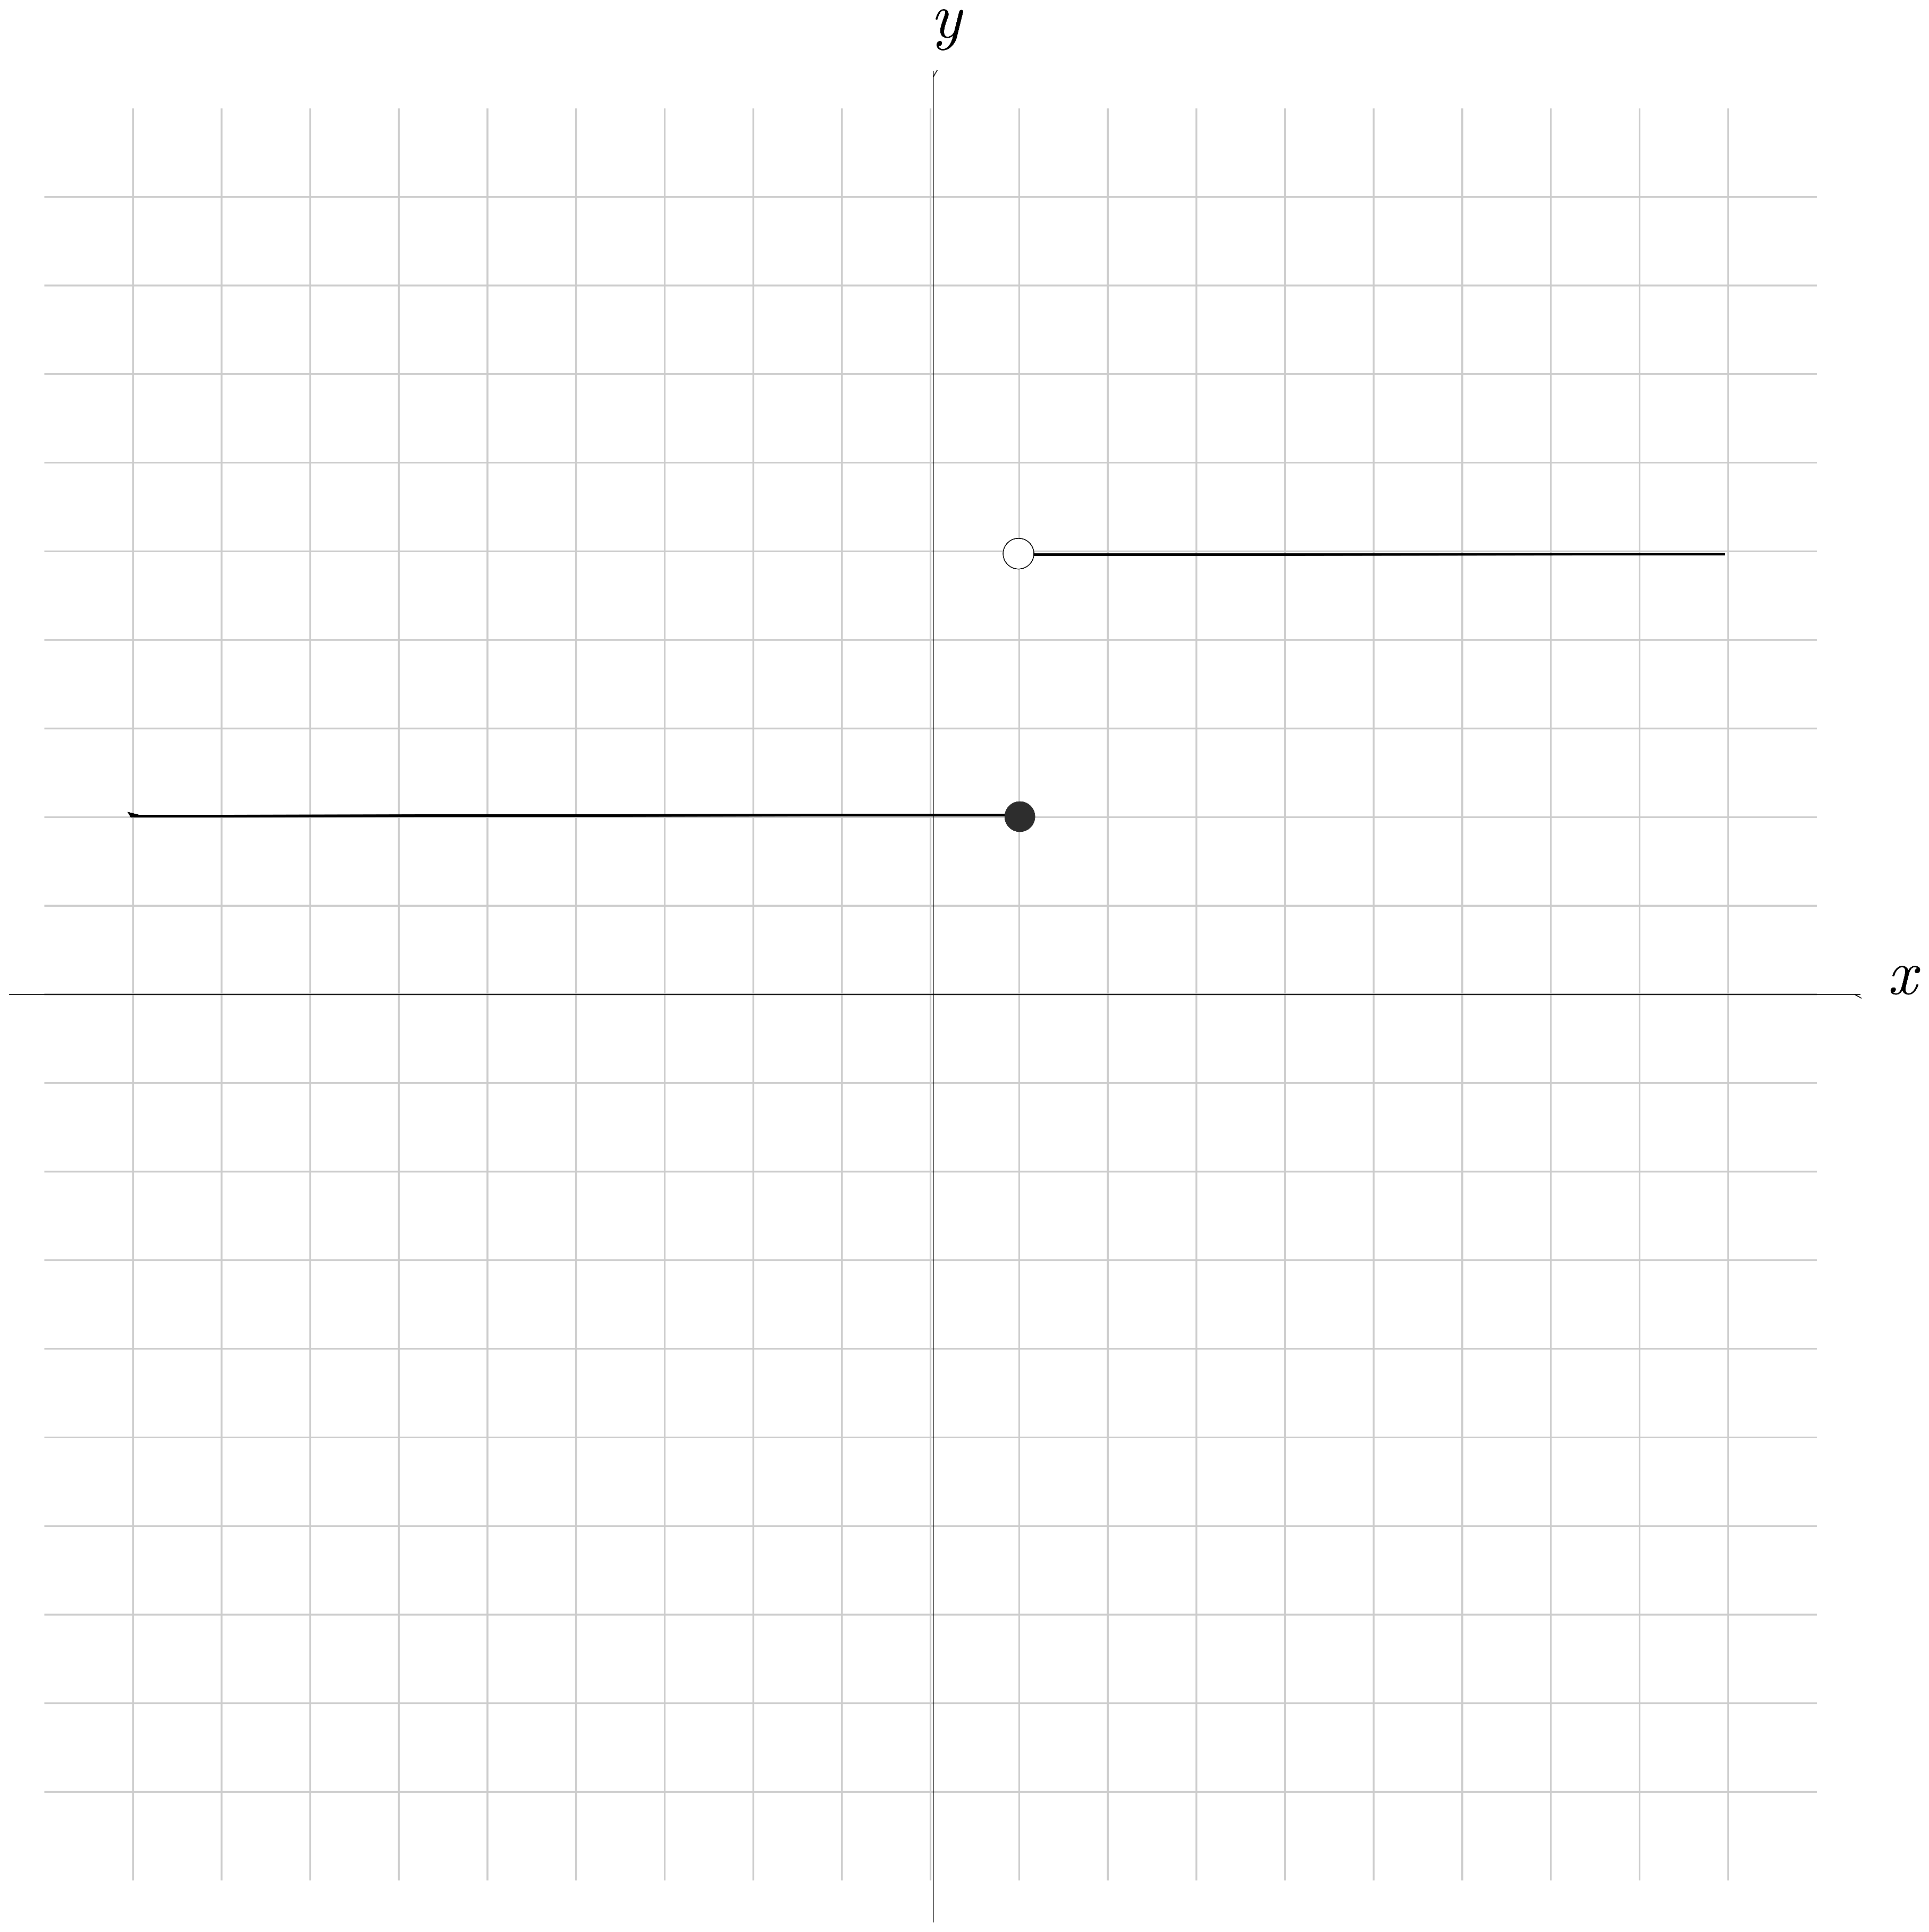
\includegraphics[width=0.3\textwidth]{continuous/limits/jumps}
  \end{center}
  \caption{A jump discontinuity.}
\end{figure}
\subsection{Side Limits}\index{side limits}

In places where a limit does not exist, we can still talk about the limit from just one side or another.
Note, however, that if $\lim_{x\to a}f(x)$ at a point, then the left an right limits also exist and must be equal to one another.

\begin{theorem}
  \( \lim_{x\to a^-} f(x)=L \) iff \(f(x)\) gets arbitrarily close to \(L\) as \(x\) comes sufficiently close to \(a\), but \(x < a \).
  \label{theorem:lefthandlimit}
\end{theorem}
\begin{figure}[H]
  \begin{center}
    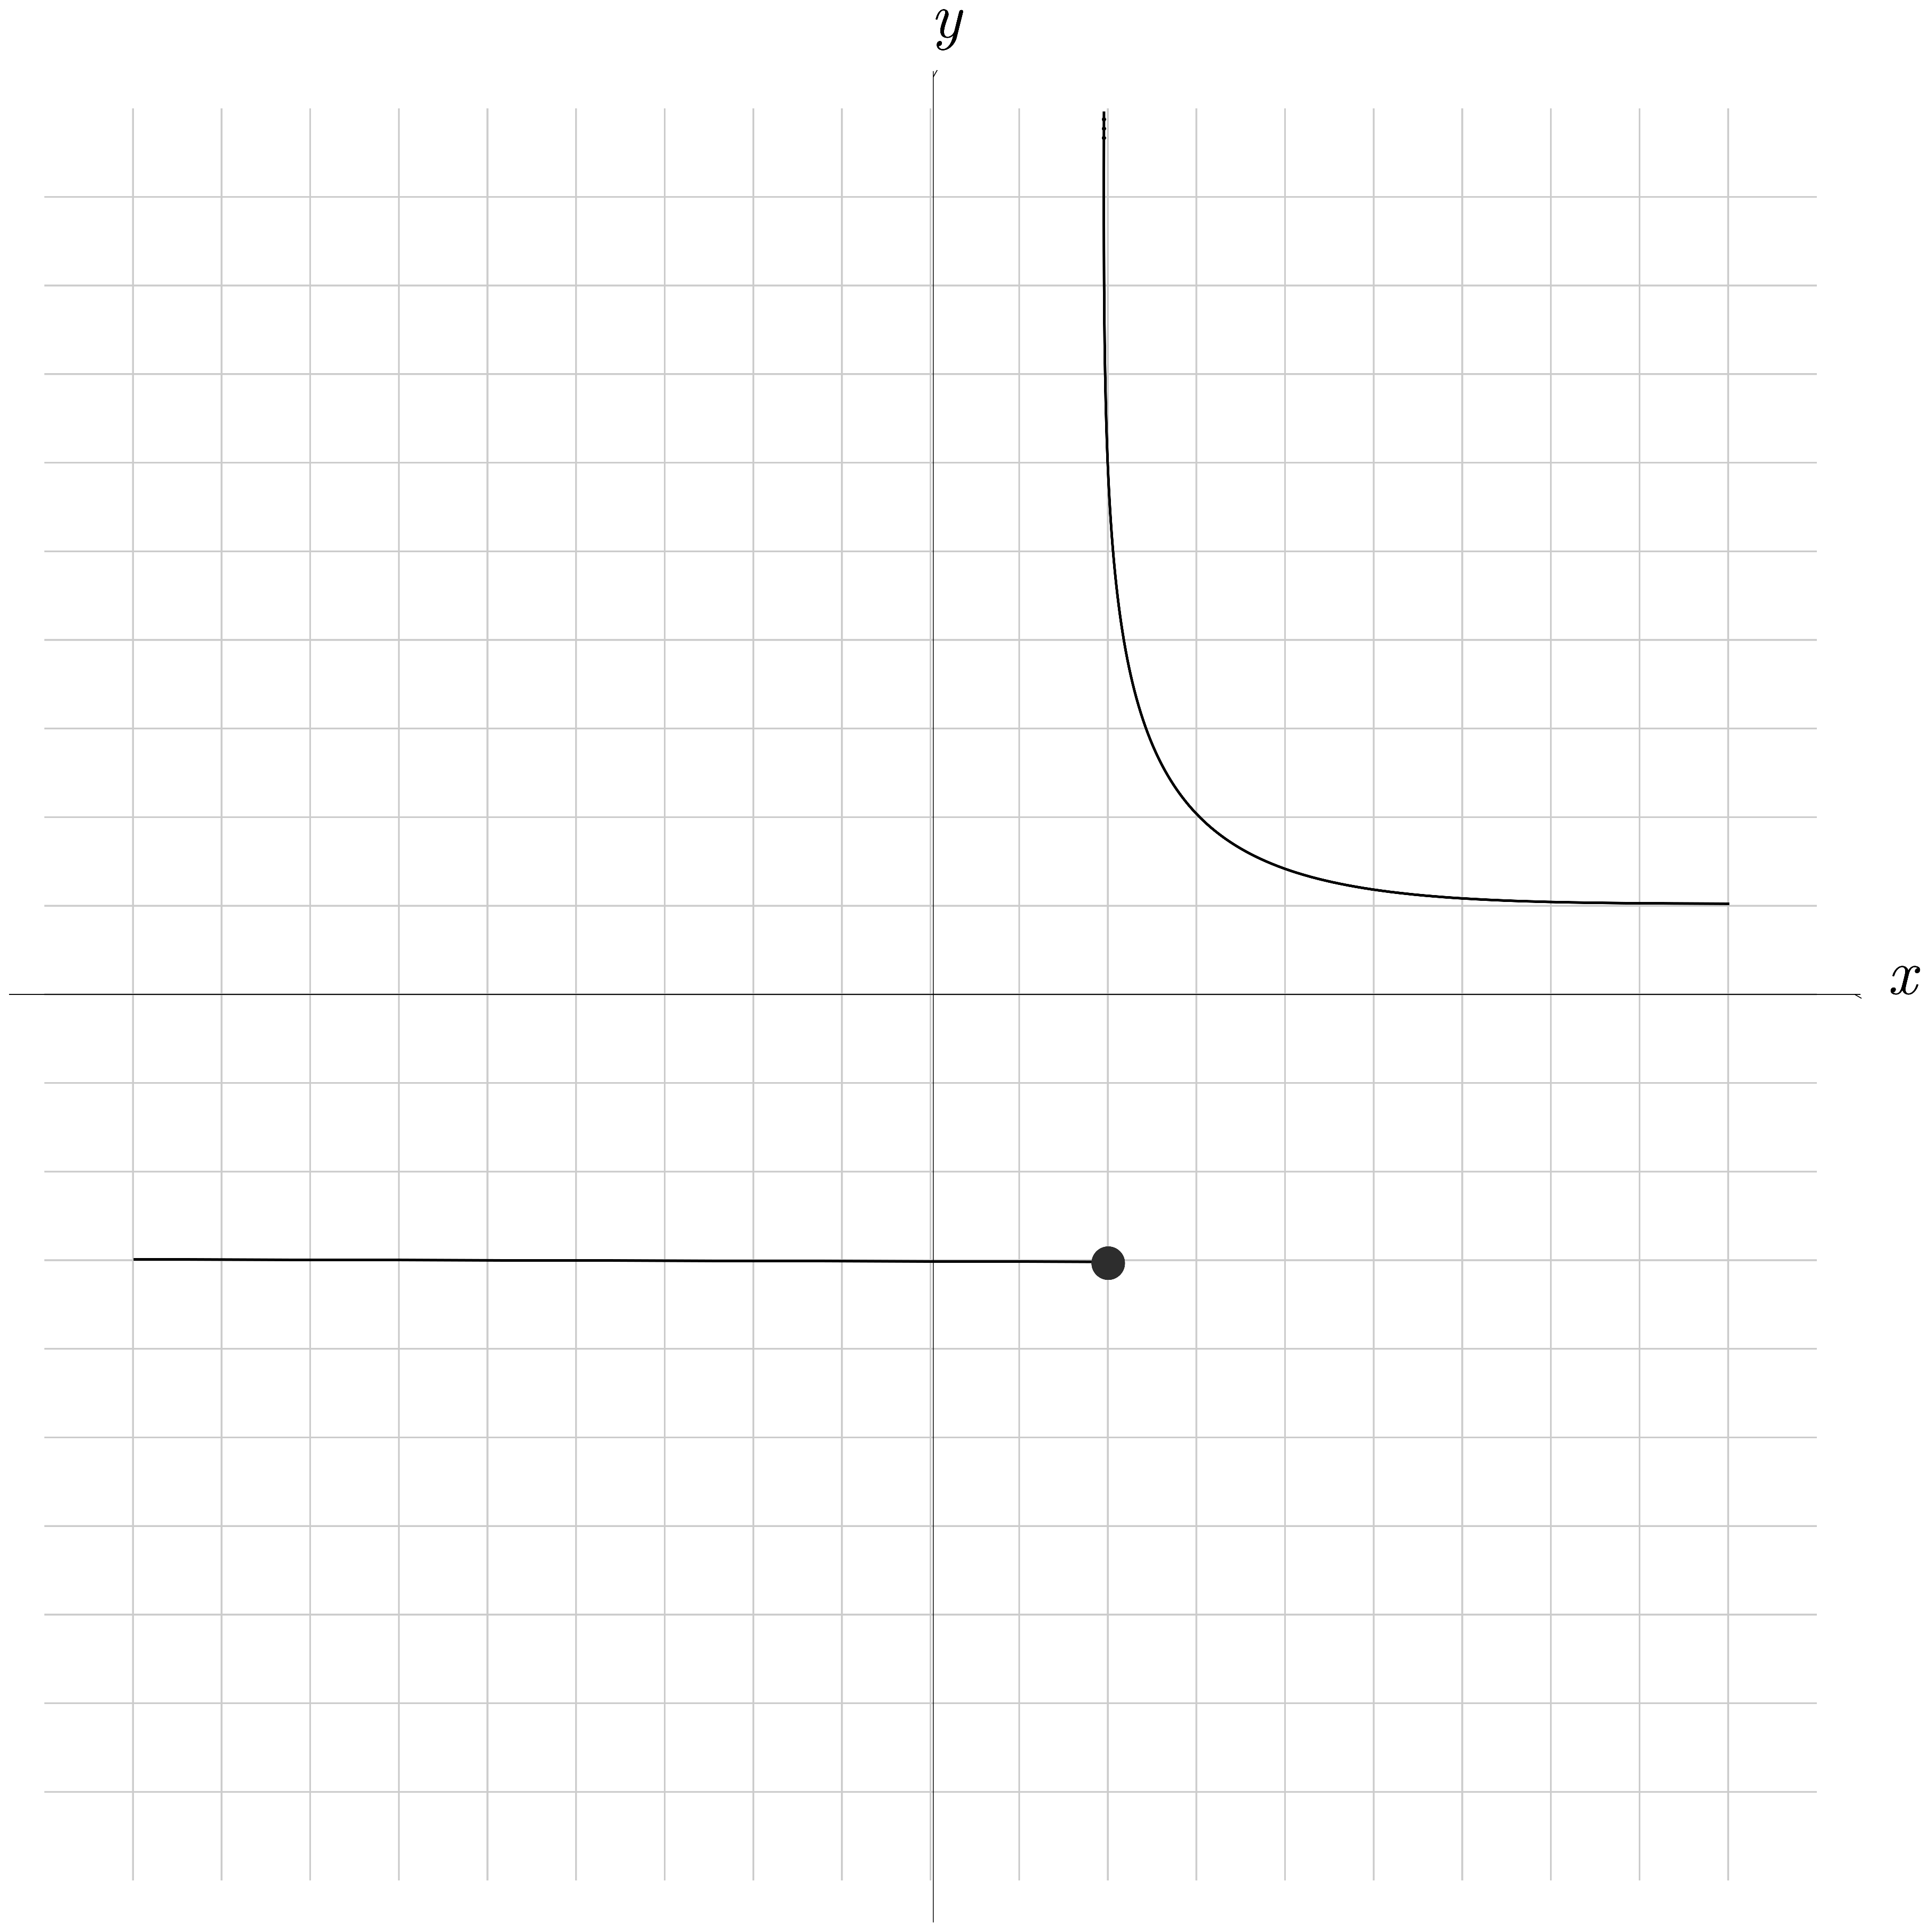
\includegraphics[width=0.5\textwidth]{continuous/limits/llmt}
  \end{center}
  \caption{The lefthand limit at $x=2$ exists, though the righthand limit does not.}
\end{figure}
\begin{theorem}
  \( lim_{x \to a^+} f(x)=L \) iff \(f(x)\) gets arbitrarily close to \(L\) as \(x\) gets sufficiently close to \(a\), but \(x > a\).
  \label{}
\end{theorem}
% section ref: Thomas' Calculus, Chapter 1

\subsection{The Sandwich Theorem}

Let us look at a more complicated example of a limit.
Suppose we have the functions
\begin{align*}
  h(x) &= |x|, \\
  f(x) &= x\sin{\frac{1}{x}}, \\
  \text{and }g(x) &= -|x|,
\end{align*}
where at \(x=0\), \(g(x) \leq f(x) \leq h(x)\) at 0.
\begin{figure}[H]
  \begin{center}
    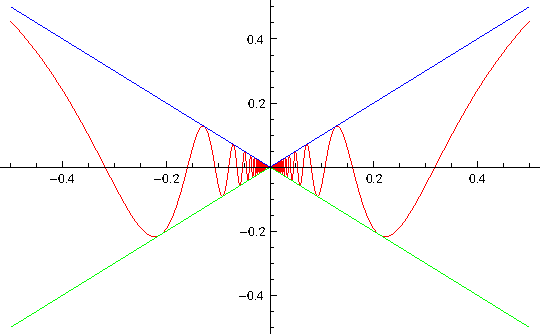
\includegraphics{graphs/sandwichtheorem.pdf}
  \end{center}
  \caption{A plot of \(h(x)\), \(f(x)\), and \(g(x)\)}
\end{figure}
We can conclude, intuitively, that the limit of \(f(x)\) as \(x \to 0\) must be
0 even though we cannot evaluate \(f(x)\) at 0, as seen in Figure
\ref{fig:p1sin1x}. We can generalize this kind of behavior as a theorem, the
\emph{sandwich theorem}.
\begin{theorem}[The Sandwich Theorem]
  If \[g(x) \leq f(x) \leq h(x)\] holds for all \(x \neq c\) in some open interval containing a number \(c\),
  and
  \[ \lim_{x \to c} g(x) = \lim_{x \to c} h(x) = L, \]
  then \(\lim_{x \to c} f(x)\) also equals $L$.
  \label{th:sandwich}
  \index{sandwich theorem}
\end{theorem}

\section{\emph{Epsilon}-\emph{Delta} Definition of a Limit}\index{epsilon-delta definition of a
limit}

The statement
\[ \lim_{x \to a} f(x) = L \]
is the statement
\begin{equation}
  \forall (\varepsilon > 0) \exists (\delta>0) \forall x \Big(0 < | x -a| < \delta \implies
  \big|f(x)-L\big| < \varepsilon\Big),
  \label{eq:e_d_limit}
\end{equation}
where the domain for the variables for $\delta$ and $\varepsilon$ consists of
all positive real numbers and for $x$ consists of all real
numbers.

\section{Evaluating Limits}

Let's look at a really complicated example of a limit\footnote{Credit for this example goes to Dr. Dobrescu's Math 140 class at CNU, Spring 2011.}, to make sure we truly understand them.
For piecewise-defined functions, limits can get especially interesting. Here's an example:
\index{piecewise function}

\begin{ex}
  \[ f(x)=
    \begin{dcases}
      x &: x \in \left[ -1,0 \right) \\
      -x &: x \in \left (0,1 \right) \\
      x-1 &: x \in \left[1, 2\right]
    \end{dcases}
    \]
  \begin{figure}[h]
    \begin{center}
      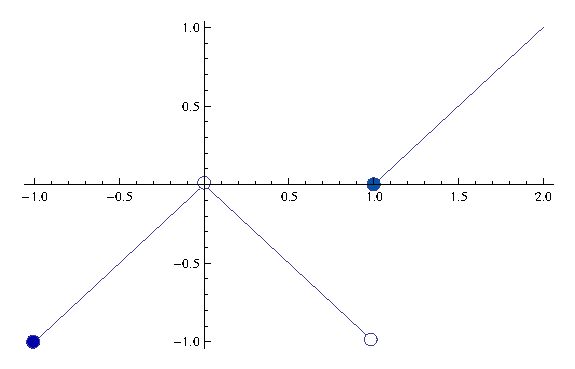
\includegraphics{graphs/pwlimex1}
    \end{center}
    \caption{A graph of \(f(x)\)}
    \label{fig:pwlimex1}
  \end{figure}
  \begin{enumerate}
    \item Does \( \lim_{x\to 0} f(x) \) exist?

      \begin{sol}
        Yes.
      \end{sol}
    \item Does \( \lim_{x \to 0} f(x)=0 \)?

      \begin{sol}
        Yes.
      \end{sol}
    \item Does \(\lim_{x \to 0} f(x)=1\)?

      \begin{sol}
        No. \(\lim_{x \to 0} f(x)=0\).
      \end{sol}
    \item Does \(\lim_{x \to 1} f(x)=1\)?

      \begin{sol}
        No. \( \lim_{x \to 1} f(x) \) does not exist.
      \end{sol}
    \item Does \(\lim_{x \to 1} f(x)=0\)?

      \begin{sol}
        No. The limit does not exist.
      \end{sol}
    \item Can we take \( \lim_{x \to x_0} f(x)\) for every \(\big(x_0 \in (-1, 1)\big)\)?

      \begin{sol}
        Yes.
      \end{sol}
    \item Does \( \lim_{x \to 1} f(x) \) exist?

      \begin{sol}
        Yes.
      \end{sol}
  \end{enumerate}
\end{ex}
\begin{ex}
  Find
  \[ \lim_{x \to 4} \frac{4x-x^2}{2-\sqrt x} \text{.} \]
  \begin{sol}
    \begin{figure}[h]
      \begin{center}
        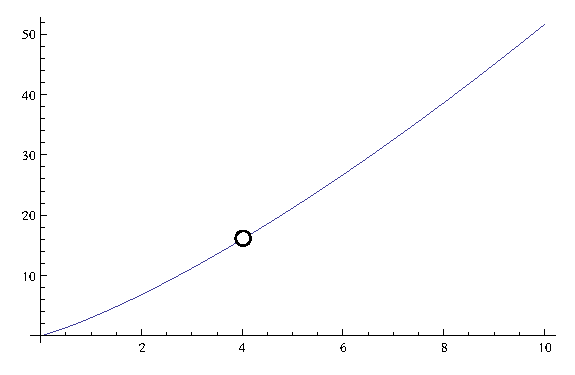
\includegraphics[width=0.4\textwidth]{continuous/limits/4xmx2}
      \end{center}
      \caption{A plot of $f(x)= \frac{4x-x^2}{2-\sqrt x}$.}
    \end{figure}
    First we multiply by the conjugate of the denominator to remove the radical from it. For more detail on conjugates, see Section \ref{app:def:conjugate}.
    \begin{align*}
      \lim_{x \to 4} \frac{4x-x^2}{2-\sqrt x}
      &= \lim_{x \to 4} \frac{4x-x^2}{2-\sqrt x} \cdot \frac{2+\sqrt x}{2+\sqrt x}\\
      \intertext{Then we simplify.}
      &=\lim_{x \to 4} \frac{x\big(4-x\big)\big(2+\sqrt{x}\big)}{4-x}
       = \lim_{x \to 4} \frac{x\big(2+\sqrt{x}\big)}{1} \\
      &= 16
    \end{align*}
  \end{sol}
\end{ex}
\begin{ex}
  Evaluate
  \[ \lim_{x \to -1} \frac{\sqrt{x^2+8}-3}{x+1} \text{.} \]
  \begin{sol}
    \begin{align*}
      \lim_{x \to -1} \frac{\sqrt{x^2+8}-3}{x+1}
      &= \lim_{x \to -1} \frac{\sqrt{x^2+8}-3}{x+1} \cdot \frac{\sqrt{x^2+8}+3}{\sqrt{x^2+8}+3}
      = \lim_{x \to -1} \frac{x^2+8-9}{(x+1)(\sqrt{x^2+8}+3} \\
      &= \lim_{x \to -1} \frac{(x-1)(x+1)}{(x+1)(\sqrt{x^2+8}+3)}
      = \lim_{x \to -1} \frac{x-1}{\sqrt{x^2+8}+3} \\
      &= \frac{-1}{3}
    \end{align*}
  \end{sol}
\end{ex}
\begin{ex}
  Suppose we wished to evaluate the limit
  \[  \lim_{\theta \to 0} \frac{\sin \theta}{5 \theta}. \]
  \begin{sol}
    Well, first we should recognize that $\sin \theta$ is not the kind of function that is growing indefinitely:
    it oscillates forever between two values, $1$ and $-1$.
    \begin{figure}[H]
      \begin{center}
        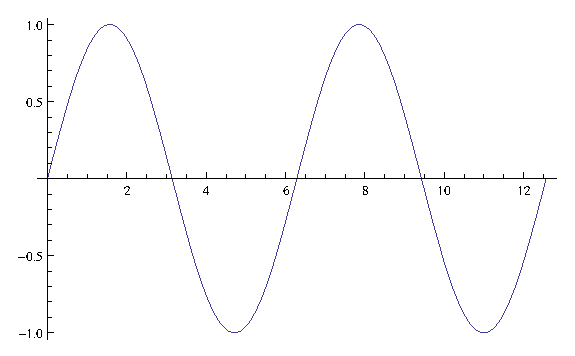
\includegraphics[width=0.5\textwidth]{continuous/limits/sintheta}
      \end{center}
      \caption{A plot of $\sin \theta$.}
      \label{fig:sintheta}
    \end{figure}
  \end{sol}
  But dividing by larger and larger values is going to make this function's \textbf{amplitude}\index{amplitude},
  its distance from the $y$-value of $0$, much smaller.

  Using Theorem \ref{th:sandwich},\footnote{How?} we can see that this limit approaches $1$.
\end{ex}

\section{Indeterminate Forms}

If we want to know how the function
$$F(x)=\frac{x-\sin x}{x^3}$$
behaves \emph{near} $x=0$ (where it is undefined), we can examine the limit of $F(x)$ as $x \to 0$. We cannot apply the Quotient Rule for limits because the limit of the denominator is $0$. Moreover, in this case, \emph{both} the numerator and denominator approach $0$, and $0/0$ is undefined. Such limits may or may not exist in general, but the limit does exist for the function $F(x)$ under discussion by applying l'Hospital's Rule, which is detailed further in Section \ref{sec:lhospital}.

If the continuous functions $f(x)$ and $g(x)$ are both zero at $x=a$, then
$$\lim_{x \to a} \frac{f(x)}{g(x)}$$
cannot be found by substituting $x=a$. The substitution produces $0/0$, a meaningless expression, which we cannot evaluate. We use $0/0$ as a notation for an expression known as an \textbf{indeterminate form}. Other meaningless expressions often occur, such as $\infty / \infty$, $\infty \cdot 0$, $\infty - \infty$, $0^0$, and $1^{\infty}$, which cannot be evaluated in a consistent way; these are called indeterminate forms as well.

\section{Continuity of Functions}
\begin{defn}
  A function is \textbf{continuous}\index{continuous} at $x=a$ iff
  \begin{itemize}
    \item $f(a)$ is defined.
    \item $\lim_{x\to a} f(x)$ exists.
    \item $\lim_{x\to a} f(x)=f(a)$.
  \end{itemize}
\end{defn}

\section{The Mean Value Theorem}
\index{mean value theorem}
The following is a simplified case of the mean value theorem:
The \textbf{mean value theorem} states that, for a continuous function $f$,
if we have an $f(a)$ which is negative and a $f(b)$ which is positive,
then $f$ crosses the $x$-axis somewhere on the interval $(a, \, b)$.

\chapter{Derivatives}

\section{Slopes}

The entire idea of a derivative is based on the idea behind the slope of a graph. You probably remember the equation for the slope of a line from algebra,
\begin{equation}
  \label{eq:slope}
  m=\frac{\Delta y}{\Delta x}=\frac{y_2-y_1}{x_2-x_1}
\end{equation}
which is usually associated with the general form of a linear equation
\begin{equation}
  y=mx+b
\end{equation}
\begin{figure}[h]
  \begin{center}
    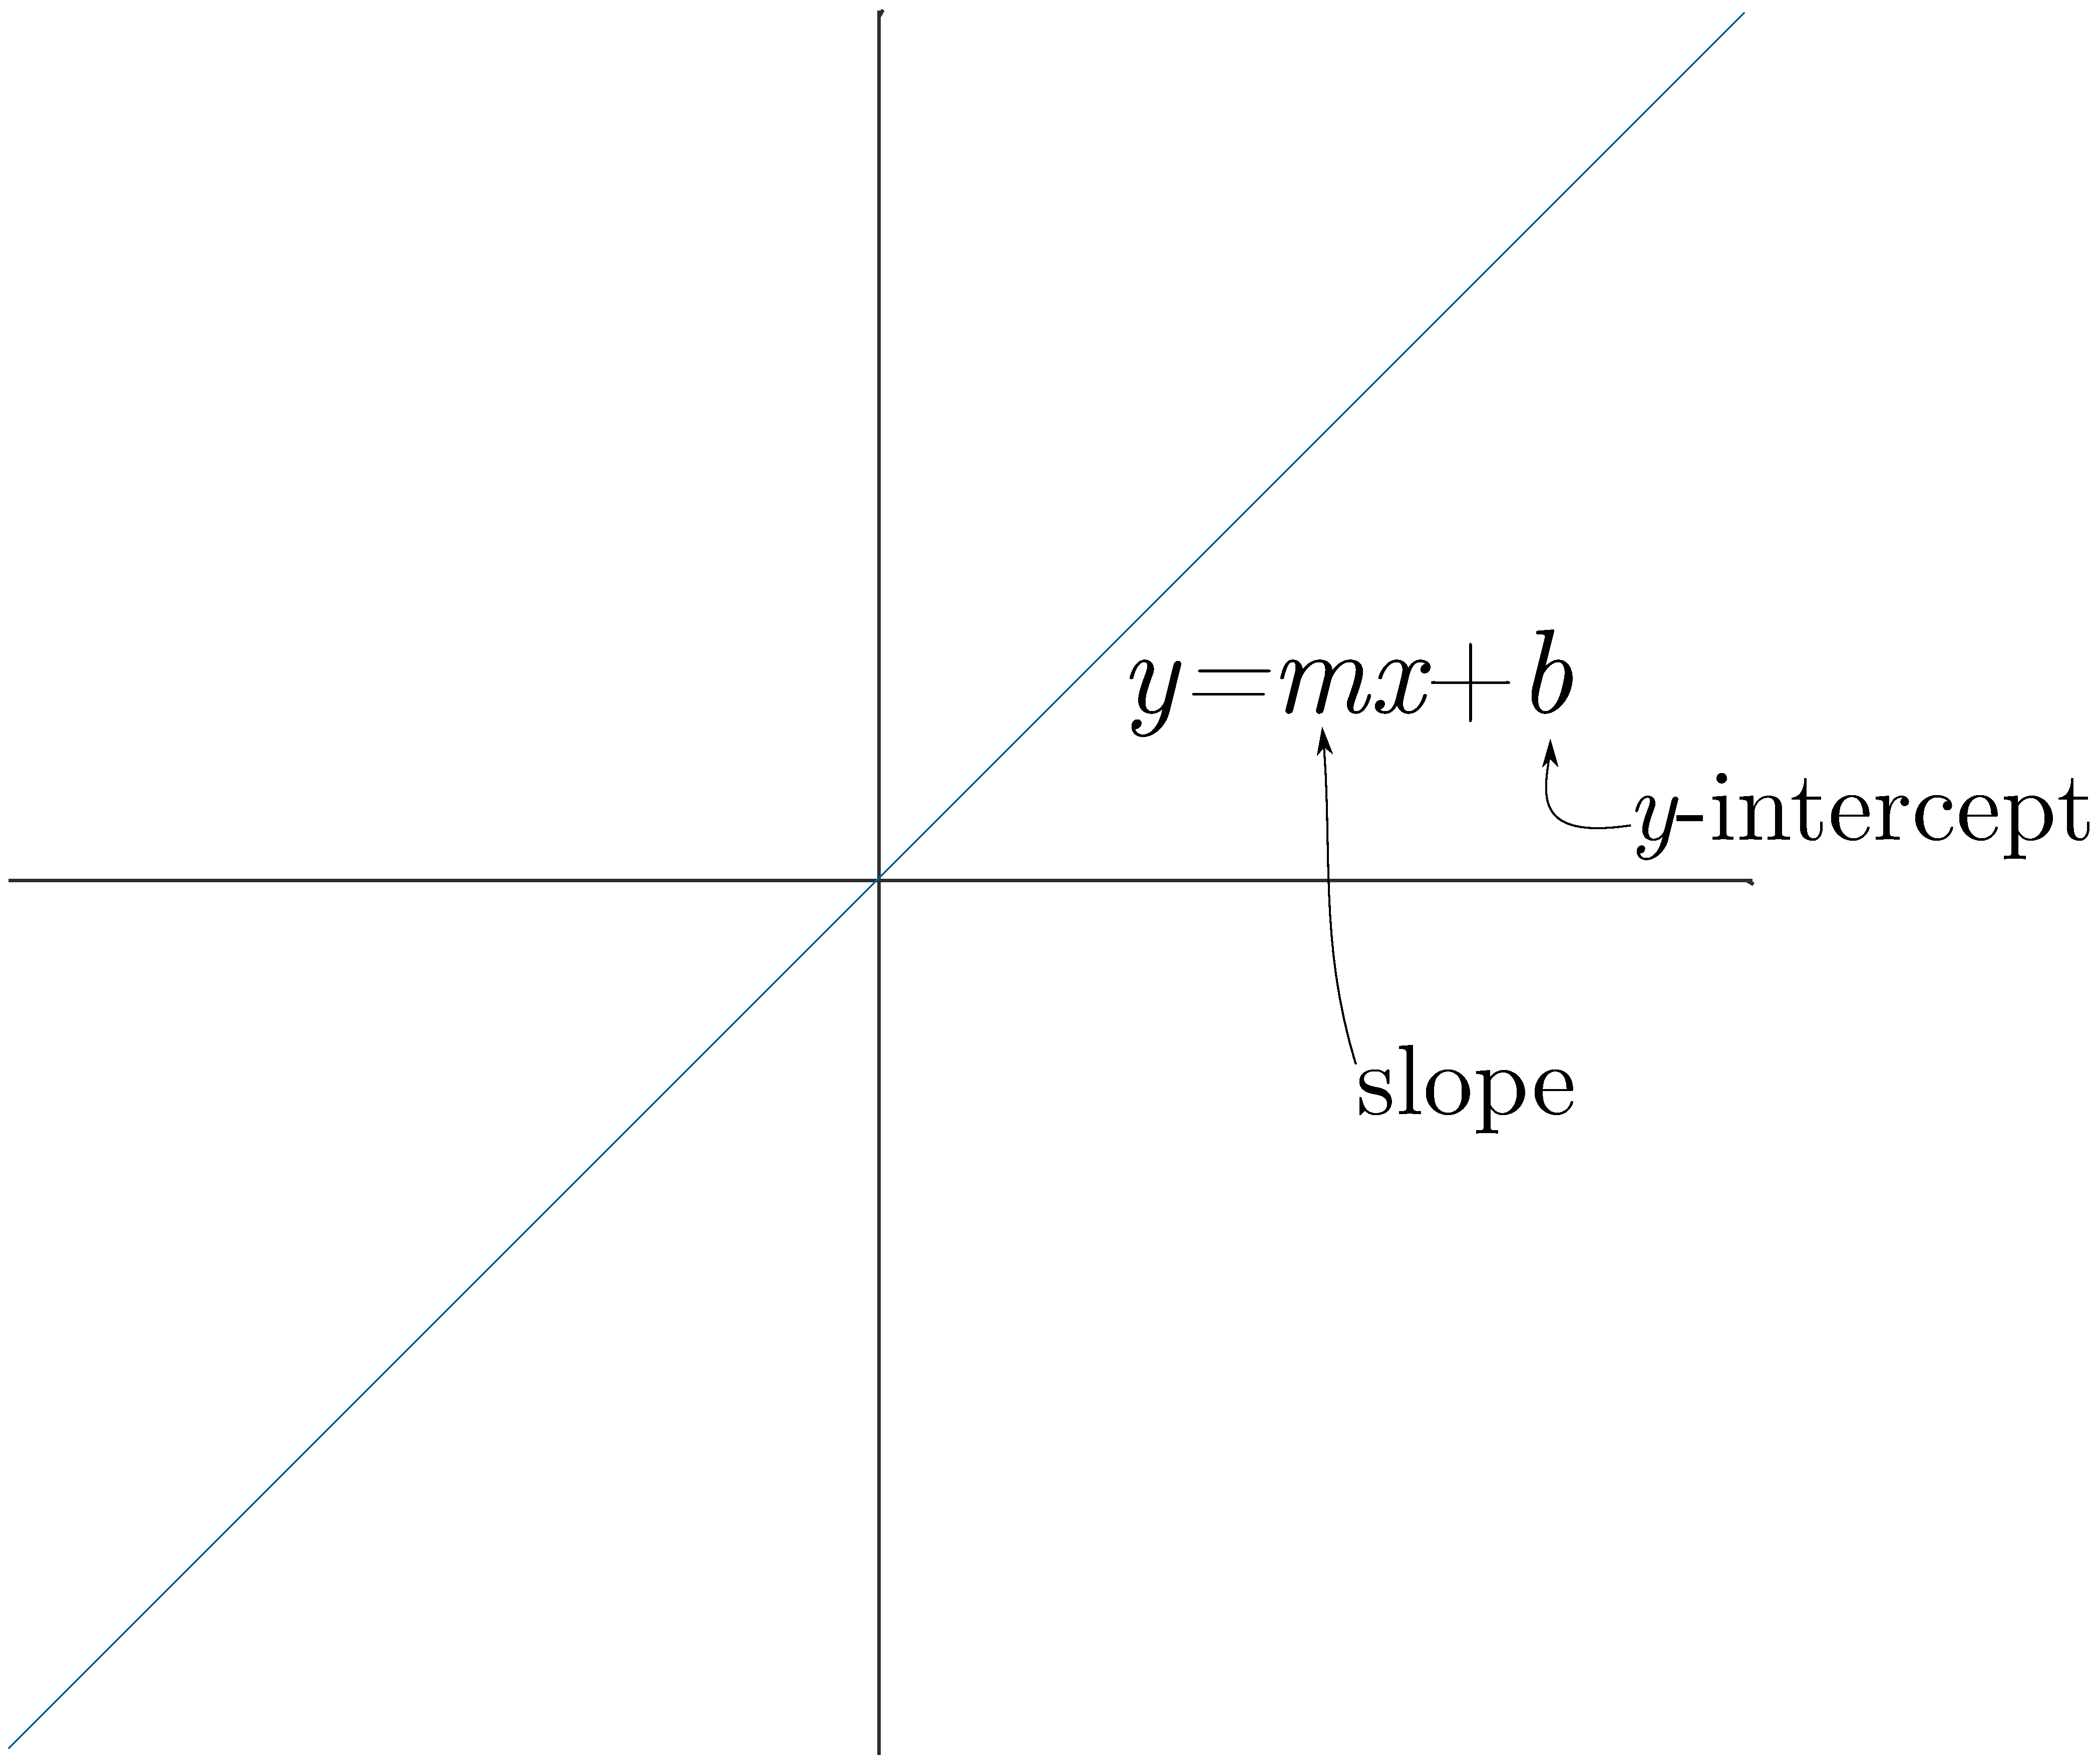
\includegraphics[width=0.5\textwidth]{continuous/derivatives/lineform.eps}
  \end{center}
  \caption{The general form equation for a line.}
\end{figure}
\begin{figure}[h]
  \begin{center}
    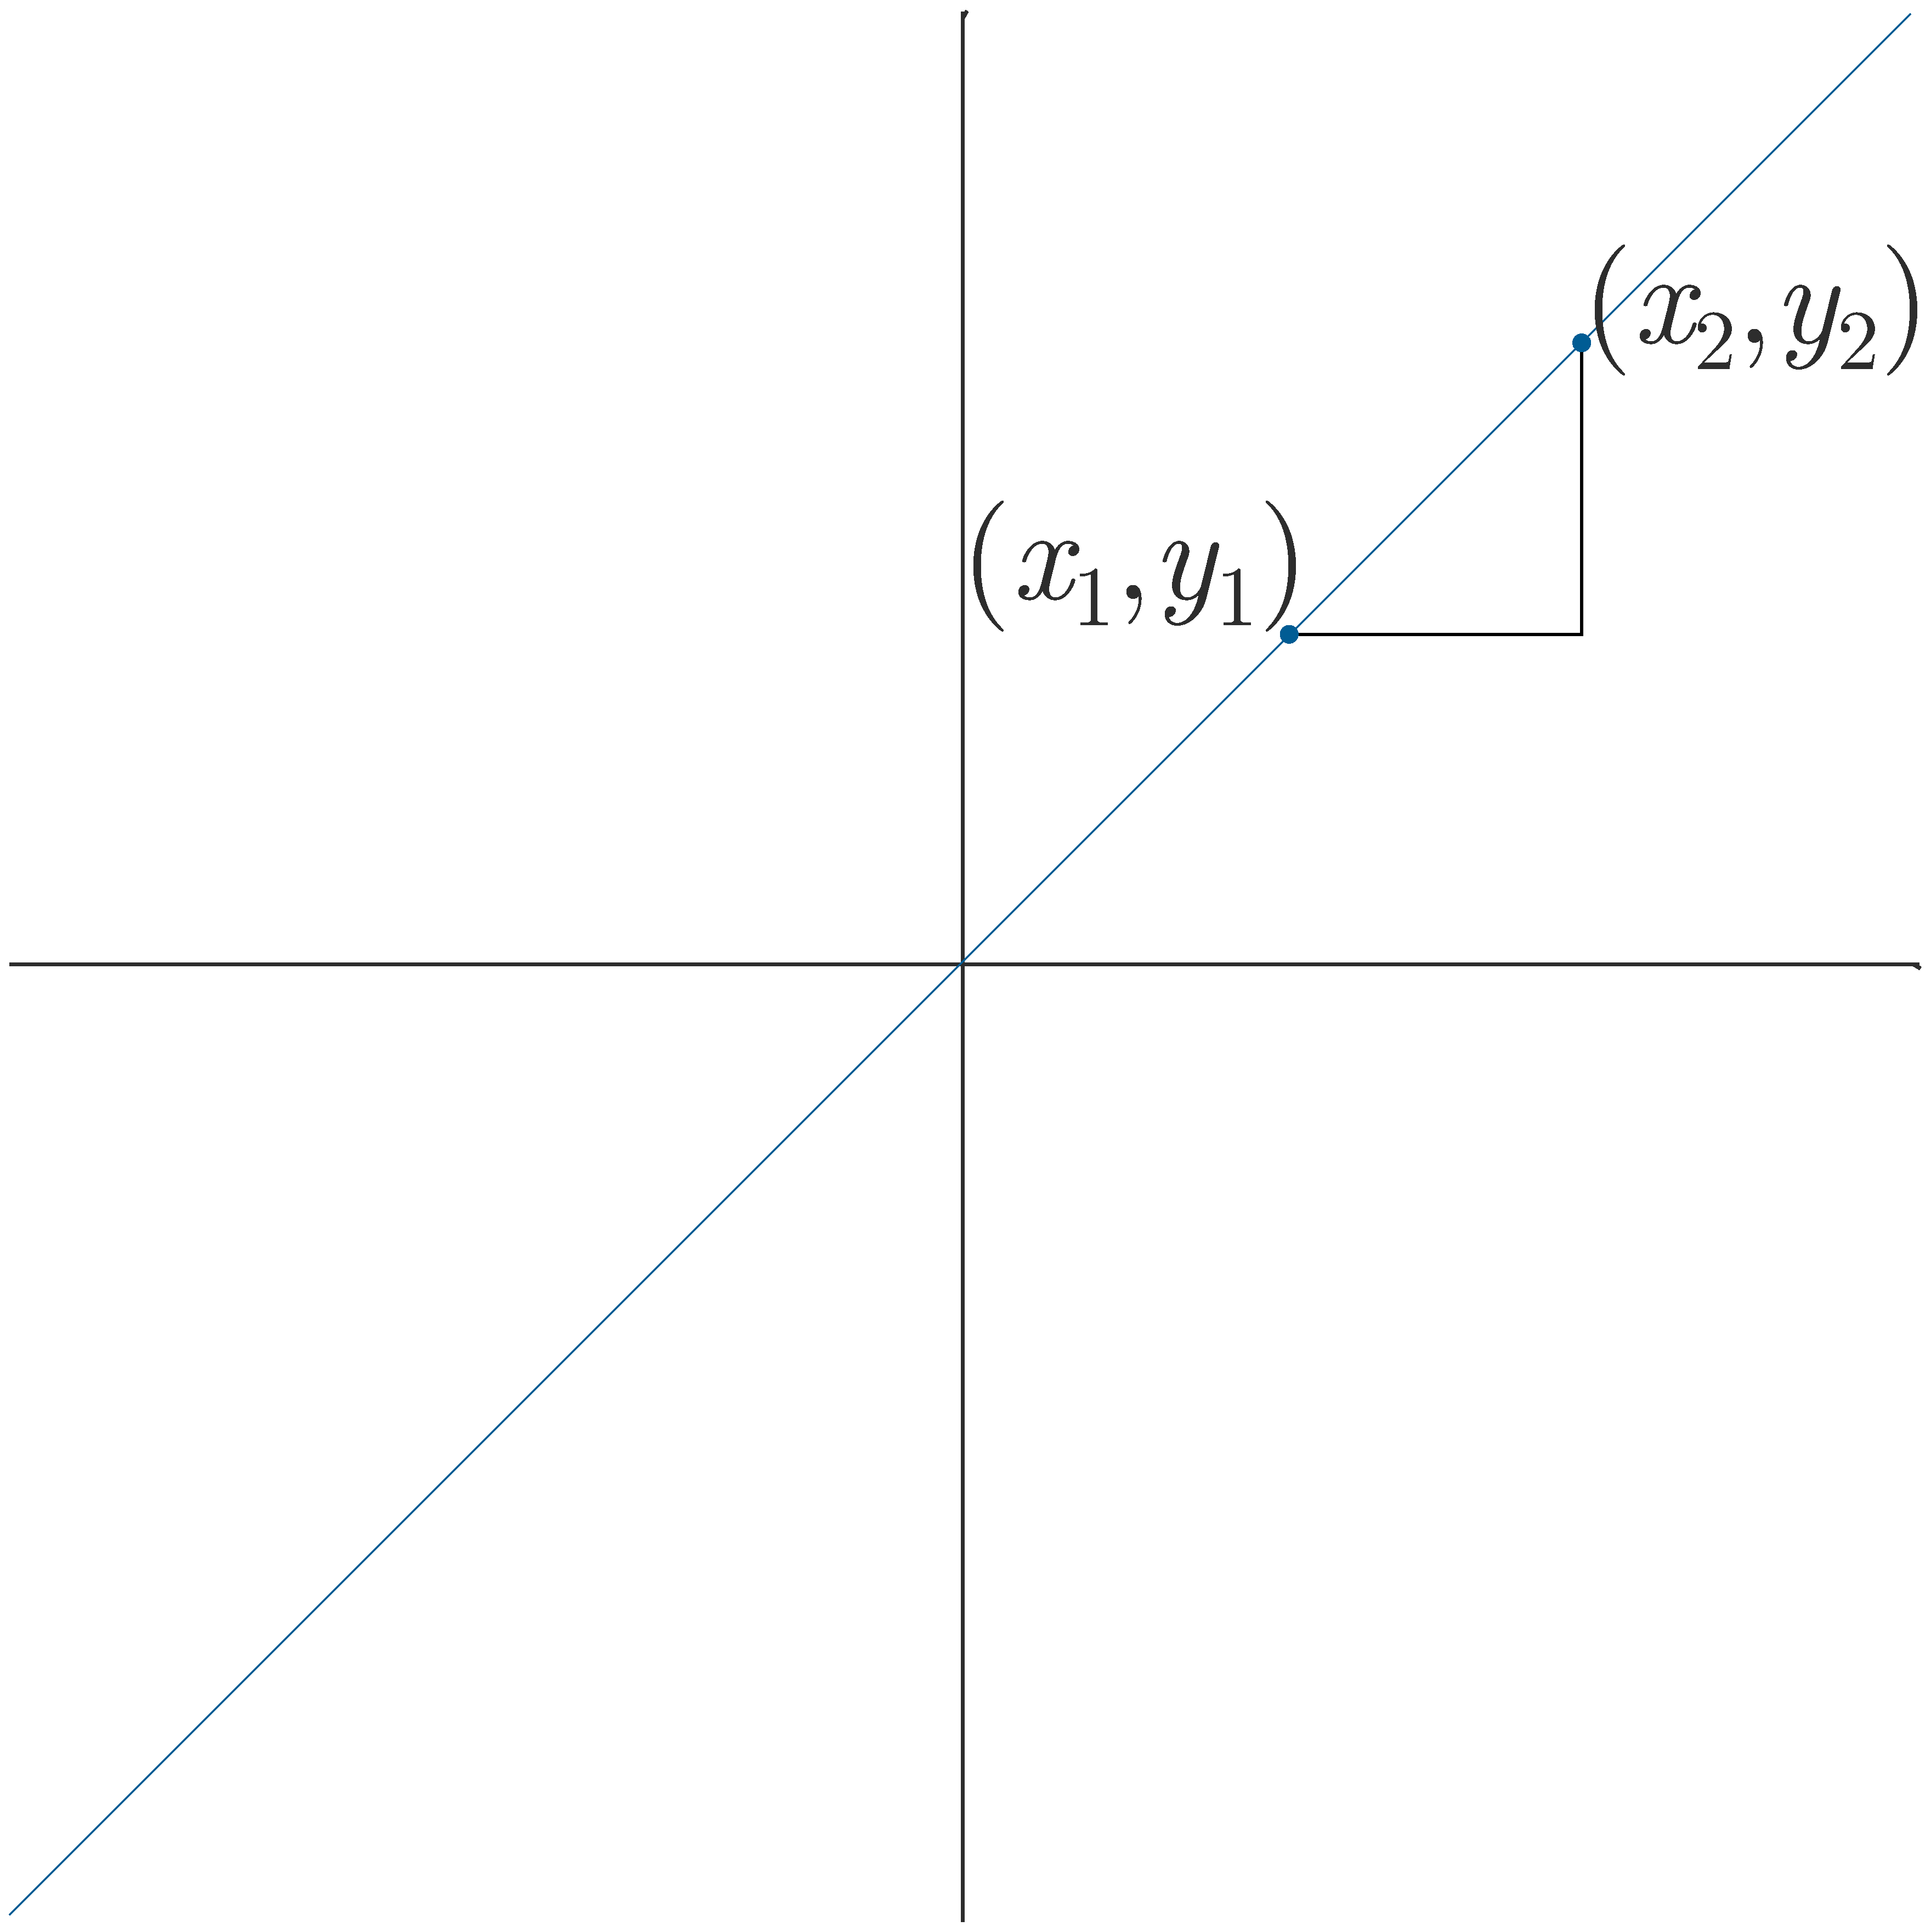
\includegraphics[width=0.5\textwidth]{continuous/derivatives/lineform_slope.eps}
  \end{center}
  \caption{How we determine ``rise over run'' in a graph.}
\end{figure}
\begin{remark}
  $\Delta$ is a common symbol in calculus, and it basically means ``change in.''
\end{remark}

Where $m$ is the slope of the graph, $x$ is your input value, and $b$ is the \emph{y-intercept}, or initial $y$ value, for the function.

Slope is also often seen with the point-slope formula, where given a point $(x_1, y_1)$ and a slope $m$, you can solve for $y$ to get a linear function.
\begin{equation}
  \label{eq:pointslope}
  y-y_1=m(x-x_1)
\end{equation}

In early mathematics courses, slope is often described as the ``rise'' over ``run'' of a graph.
While this is accurate, it doesn't provide the complete picture.
What a \emph{slope} really describes is how much a given function $f(x)$ is altering each of its input values $x$, often heard as ``change in $y$ over change in $x$.''
You'll notice that this is independent of any initial value $b$ selected for a linear function.\footnote{Which is why all constants disappear when you take the derivative of a function.}

To figure out the slope of a linear function $f(x)=mx+b$, all you need to do is
divide the difference between two output ($y$) values by the difference between
their two input ($x$) values. This is where equation \eqref{eq:slope} comes from:
\begin{equation*}
  m=\frac{f(x_2)-f(x_1)}{x_2-x_1}
\end{equation*}
And because the function is linear, the slope $m$ is constant all the way through and any two points can be used to find it.

\section{The Difference Quotient}\index{Difference Quotient}

The \emph{difference quotient} is the same exact thing as the slope formula, with the only distinction
being you treat how far apart your two $x$ values are as a variable. So $\Delta x=x_2-x_1$, and $x=x_1$.
\begin{equation}
  \frac{\Delta f(x)}{\Delta x}=\frac{f(x+\Delta x)-f(x)}{\Delta x}
\end{equation}
\begin{figure}[h]
  \begin{center}
    
\includegraphics[width=0.5\textwidth]{continuous/derivatives/diffquot.eps}
  \end{center}
  \caption{A visual representation of the difference quotient on a line.}
\end{figure}
You'll often see the difference quotient written with $\Delta x \to h$ as
\begin{equation}
  \frac{\Delta f(x)}{\Delta x}=\frac{f(x+h)-f(x)}{h}
\end{equation}

\section{Derivatives}

\subsection{Limit Definition}

The difference quotient is used in the limit definition of the derivative, which is
\begin{equation}
  \label{eq:limitdef}
  \frac{\ud f(x)}{\ud x}=\lim_{h \to 0} \frac{f(x+h)-f(x)}{h}
\end{equation}
Notice that the only distinction between this equation and the difference quotient/slope equation from earlier is the introduction of a limit. The idea behind that limit is that you're calculating the slope of a function as the distance between your $x_2$ and $x_1$ values becomes infinitely small ($h\to 0$). We call this distance an \emph{infinitesimal}: a distance smaller than any feasible measurement, but not zero in size.

So what a derivative of a function is going to tell us is how the function behaves (its slope) at a particular ``infinitely small'' portion of the graph, which might as well be a point.

For linear functions, the function behaves the same no matter where you look at it, so their derivatives are always constant and equal to the slope of the function.

For nonlinear functions, like $f(x)=x^2$, the derivative will yield a function (in this case, just $f'(x)=2x$), because the function is changing its input values differently depending on where you are looking. Near the origin, where $x=0$, the derivative is zero and any $x$ value will give $y$ values not too far from the original input. But as you move further from the origin, the ratio of $y/x$ gets larger and larger, and the derivative in turn gets bigger and bigger.

\begin{figure}[H]
    \begin{center}
      
\includegraphics[width=0.5\textwidth]{continuous/derivatives/xsquared.eps}
      \caption{A graph of $f(x)=x^2$ and $f'(x)=2x$.}
    \end{center}
  \end{figure}

\subsection{Notation}

There are a number of ways to denote the derivative of a function $y=f(x)$. The most common notation early on in calculus classes is the \emph{prime} notation $y'$ and $f'$ because it is the simplest. Later on, you often see $\ud/\ud x$ style notation, because it is more specific. It tells us not only which function we are differentiating, but with respect to which variable. A notable characteristic of this ``d notation'' is the similarity it provides to our equation for slope:
\begin{align*}
  &m=\frac{\Delta y}{\Delta x}=\frac{\Delta f(x)}{\Delta x} &y'=\frac{\ud y}{\ud x}=\frac{\ud f(x)}{\ud x}
\end{align*}
In the case of slope, we're talking about specific $y$ and $x$ values, but in the case of a derivative, we're talking about \emph{infinitesimals}, and that particular distinction allows us to discuss the behavior of functions that aren't linear, but change their behavior over time.

\subsection{Tangent Lines}

The \emph{tangent line} to a graph at a point is just a line that acts like the function is linear and behaves exactly as the graph does at that point. This is useful for visualizing the derivative, and showing us how the behavior of a function can change depending on its $(x,y)$ location.

\begin{figure}[H]
  \begin{center}
    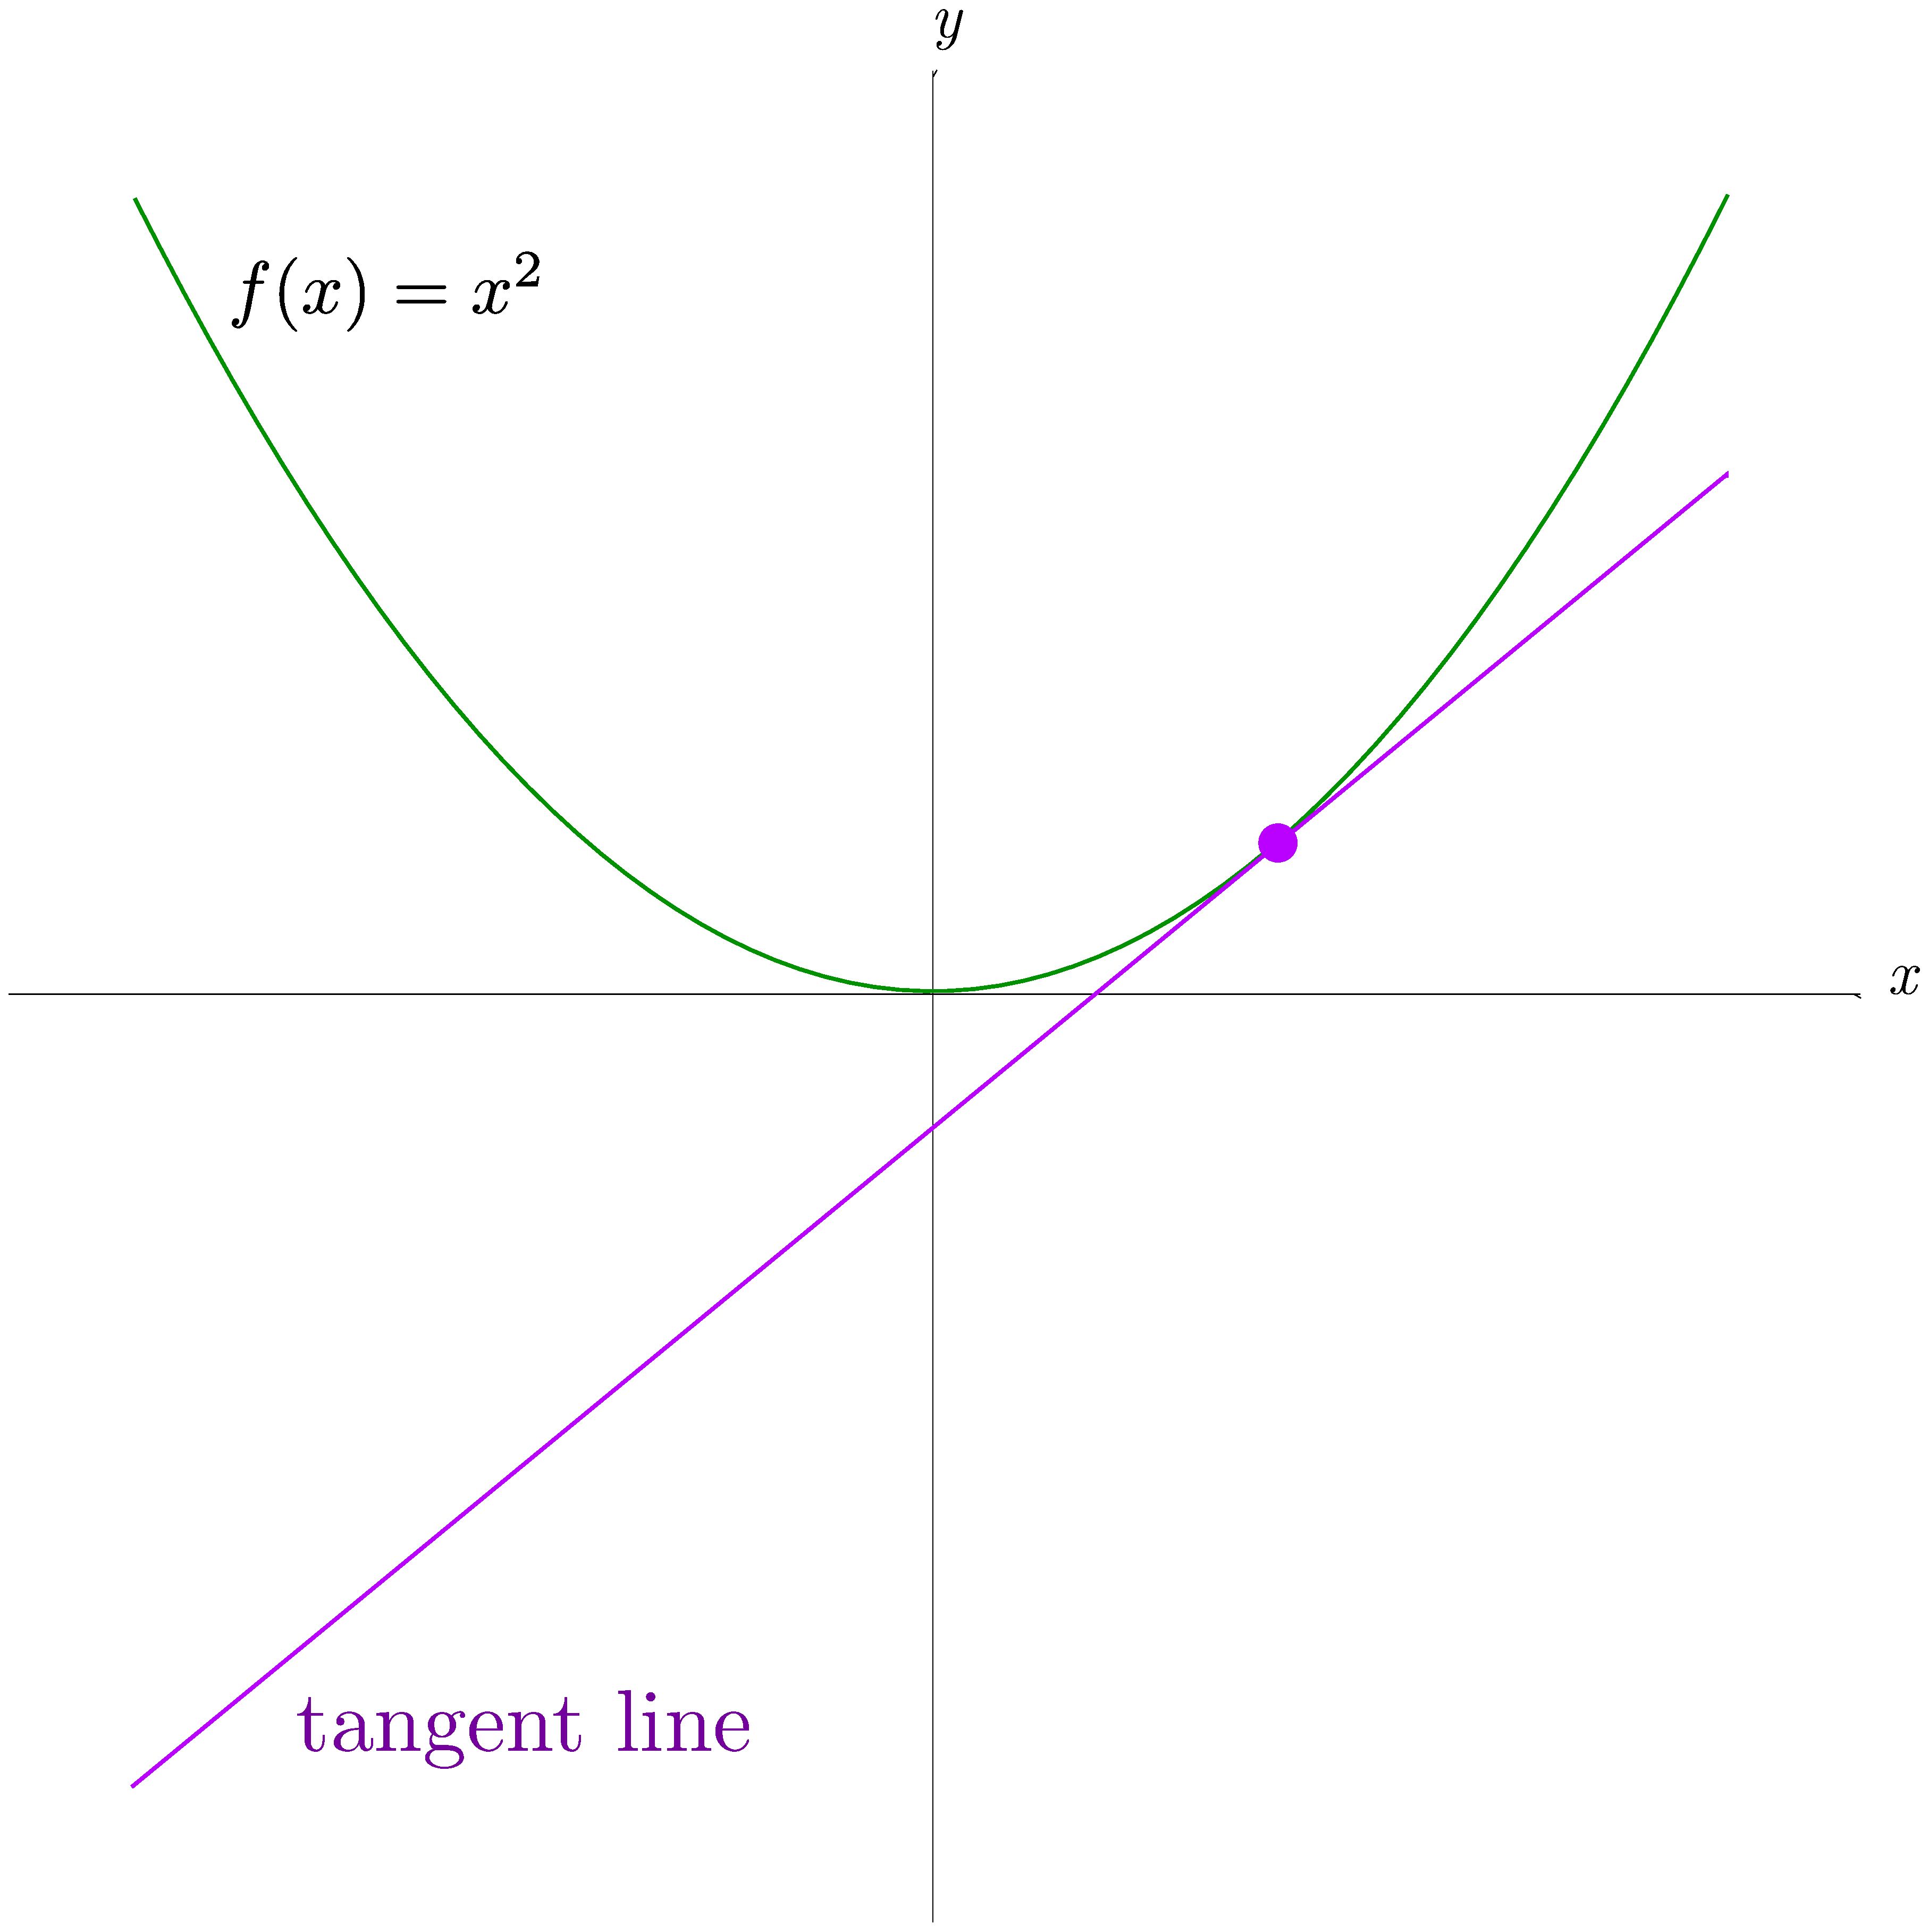
\includegraphics[width=0.4\textwidth]{continuous/derivatives/tangent.eps}
  \end{center}
  \caption{A tangent line to the graph of $f(x)=x^2$.}
\end{figure}

To calculate the equation for a tangent line at a point, simply find the
derivative of the function at that point and treat that as the slope of the
tangent line. Then, use the $(x, y)$ values of the point to produce the tangent line's function
using the point-slope equation (\eqref{eq:pointslope}).

\subsection{Derivative Rules}

Derivative rules are just shorthands for working things out manually using the
limit definition in equation \eqref{eq:limitdef}. They all come from equation \eqref{eq:limitdef}, but they serve as generalizations to greatly simplify the work we have to do in calculating derivatives.

\subsubsection{Power Rule}

The power rule states that
\begin{equation}
  \ddx x^n=nx^{n-1}
\end{equation}

\subsubsection{Product Rule}

The product rule states that
\begin{equation}
  \ddx (uv)=u \frac{\ud v}{\ud x}+v\frac{\ud u}{\ud x}
\end{equation}

\subsubsection{Quotient Rule}

The quotient rule states that
\begin{equation}
  \frac{\ud}{\ud x}\left(\frac{u}{v}\right)=\frac{v\frac{\ud u}{\ud x}-u\frac{\ud v}{\ud x}}{v^2}
\end{equation}

\subsubsection{Chain Rule}

The chain rule states that if $y=f(u)$ and $u=g(x)$, then
\begin{equation}
  \frac{\ud y}{\ud x}=\frac{\ud y}{\ud u} \cdot \frac{\ud u}{\ud x}
\end{equation}

The chain rule is used to differentiate composite functions, which look like $(f \circ g)(x)$ and mean $f(g(x))$. You'll want to develop an intuitive understanding for when to use the chain rule.
\begin{ex}
  Find the derivative of $f(x)$, where
  \[ f(x)=\frac{1}{x^3} \]
  \begin{figure}[h]
    \begin{center}
      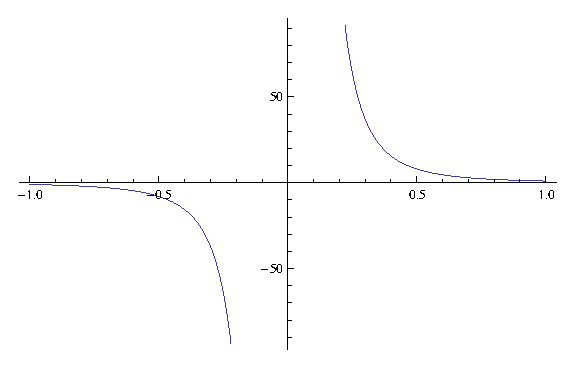
\includegraphics{continuous/derivatives/chainrule_1.eps}
    \end{center}
    \caption{A plot of $f(x)=\frac{1}{x^3}$.}
  \end{figure}
  \begin{sol}
    This is not a chain rule problem. Although you could think of it as one with $f(x)=1/x$ and $g(x)=x^3$, it is easier to remember that factors can be moved from the numerator to the denominator simply by multiplying their exponents by $-1$.
    \begin{align*}
      f(x)&=\frac{1}{x^3}\\&=x^{-3} \\
      \ddx f(x)&=-3x^{-4}
    \end{align*}
  \end{sol}
\end{ex}
\begin{ex}
  Find the derivative of $f(x)$, where
  $$ f(x)=\left(\frac{1}{\sqrt{x}}\right)^5 $$
  This is a chain rule problem. We use
  \begin{align*}
    & g(x)=\frac{1}{\sqrt{x}}
    & & f(x)={(g(x))^5}
  \end{align*}
  \begin{align*}
    \ddx f(x)&=\ddx \left(\frac{1}{\sqrt{x}}\right)^5 \\
      &= \ddx {(g(x))^5} \\
      &= 5g(x)^4 \cdot \ddx g(x)
  \end{align*}
  Now we find $ \ddx g(x) $
  \begin{align*}
    \ddx g(x) &= \ddx \frac{1}{\sqrt{x}} =\ddx \frac{1}{x^{1/2}} =\ddx x^{-1/2} \\
      &=\frac{-1}{2}x^{-3/2} =\frac{-1}{2x^{3/2}} \\
      &=\frac{-1}{2\sqrt{x^3}}
  \end{align*}
  and plug that back into our original derivative, along with $g(x)=\frac{1}{\sqrt{x}}$
  \begin{align*}
    \ddx f(x)&=5g(x)^4 \cdot \ddx g(x) \\
      &=5\left(\frac{1}{\sqrt{x}}\right)^4\cdot \frac{-1}{2\sqrt{x^3}}
  \end{align*}
  and simplify
  \begin{align*}
    \ddx f(x)&=5\left(\frac{1}{\sqrt{x}}\right)^4\cdot \frac{-1}{2\sqrt{x^3}} =5\left[\frac{1^4}{\left(\sqrt{x}\right)^4}\right] \cdot \frac{-1}{2\sqrt{x^3}} \\
    &=5\left[\frac{1}{\left(x^{1/2}\right)^4}\right] \cdot \frac{-1}{2\sqrt{x^3}}=5\left[\frac{1}{x^{4/2}}\right] \cdot \frac{-1}{2\sqrt{x^3}} \\
    &=5\left[\frac{1}{x^2}\right] \cdot \frac{-1}{2\sqrt{x^3}}=\frac{5}{x^2} \cdot \frac{-1}{2\sqrt{x^3}} \\
    &=\frac{-5}{2x^2\sqrt{x^3}} =\frac{-5}{2x^2\cdot x^{3/2}} \\
    &=\frac{-5}{2x^{4/2}\cdot x^{3/2}}\\
    &=\frac{-5}{2x^{7/2}} \\
  \end{align*}
\end{ex}
\subsection{Differentiability}
  A function $f(x)$ is differentiable at a point $x_0$ if a tangent line to its curve exists at that point and is not vertical. Functions are not differentiable at breaks, immediate bends, cusps, or places with vertical tangents.

\subsection{Graphing Functions}
To graph a function:
  \begin{enumerate}
   \item Find all \textbf{critical values}. Critical values are locations where $\frac{\ud y}{\ud x}=0$ or is undefined.\footnote{At locations where $\frac{\ud y}{\ud x}=0$, the tangent line is horizontal.}
   \item Find all \textbf{points of inflection}. These are locations where the second derivative ($\frac{\ud^2y}{\ud x}$) is zero or undefined.
   \item Determine where $\frac{\ud y}{\ud x}$ is \emph{positive} to find where $f(x)$ is \emph{increasing}. Remember that a derivative signifies the slope of a graph, so a positive derivative implies that the graph is increasing. This can be achieved either by testing values on each side of a \emph{critical value}, or by intuitive understanding. For example, $\frac{\ud y}{\ud x}=3x^2$ is positive everywhere except at $x=0$, so $f(x)=y$ is increasing everywhere except for at its horizontal tangent at $x=0$.\footnote{$x^2$ can never produce a negative number, because a negative times a negative or a positive times a positive is always positive}
   \item Determine where $\frac{\ud y}{\ud x}$ is \emph{negative} to find where $f(x)$ is \emph{decreasing}.
   \item Determine the sign of $\frac{\ud^2y}{\ud x}$ on both sides of all \emph{points of inflection}. The graph is \emph{concave up} where $\frac{\ud^2y}{\ud x}$ is positive, and \emph{concave down} where $\frac{\ud^2y}{\ud x}$ is negative.
  \end{enumerate}
\section{l'Hospital's Rule}\index{l'Hospital's Rule}

\textbf{l'Hospital's Rule} uses derivatives to calculate limits\index{limits} of fractions whose numerators and denominators both approach the same indeterminate for, which can be either zero or $\infty$. Limits involving transcendental functions\index{transcendental functions} often require some use of the rule for their calculation.

\begin{theorem}[L'Hospital's Rule]\label{th:lhospital}
  Suppose that $f(a)=g(a)=0$, that $f$ and $g$ are differentiable on an open interval $I$ containing $a$, and that $g'(x) \neq 0$ on $I$ if $x \neq a$. Then
  \[ \lim_{x \to a} \frac {f(x)}{g(x)} \=H \lim_{x \to a} \frac{f'(x)}{g'(x)} \]
  assuming that the limit on the right side of this equation exists.
\end{theorem}
\begin{remark}
  L'Hopital's Rule does not apply when either the numerator or the denominator has a finite nonzero limit.
\end{remark}
\begin{proof}
  We first establish the limit equation for the case $x \to a^+$. The method needs almost no change to apply to $x \to a^{-}$, and the combination of these two cases establishes the result.

  Suppose that $x$ lies to the right of $a$. Then $g'(x) \neq 0$, and we can apply Cauchy's Mean Value Theorem to the closed interval from $a$ to $x$. This step produces a number $c$ between $a$ and $x$ such that
  $$ \frac{f'(c)}{g'(c)}=\frac{f(x)-f(a)}{g(x)-g(a)} $$
  But $f(a)=g(a)$, so
  $$ \frac{f'(c)}{g'(c)}=\frac{f(x)}{g(x)} $$
  As $x$ approaches $a$, $c$ approaches $a$ because it always lies between $a$ and $x$. Therefore,
  $$ \lim_{x \to a^+} \frac{f(x)}{g(x)}=lim_{c \to a} \frac{f'(c)}{g'(c)} = lim_{x \to a^+} \frac{f'(x)}{g'(x)} $$
  which establishes l'Hospital's Rule for the case where $x$ approaches $a$ from
  above. The case where $x$ approaches $a$ from below is proved by applying
  Cauchy's Mean Value Theorem to the closed interval $[x,a], x <
  a$.\cite{thomas}
\end{proof}
\begin{figure}[h]
  \begin{center}
    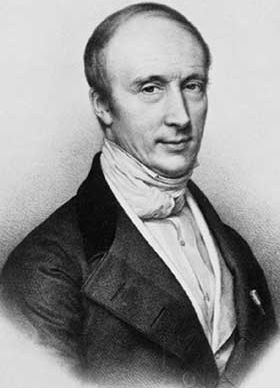
\includegraphics[width=0.2\textwidth]{photos/cauchy.jpg}
  \end{center}
  \caption{Augustin Louis Cauchy, 1901.}
\end{figure}
\begin{theorem}[Cauchy's Mean Value Theorem]\label{th:caunchymv}\index{Cauchy's Mean Value Theorem}
Suppose functions $f$ and $g$ are continuous on $[a, b]$ and differentiable throughout $(a, b)$ and also suppose $g'(x) \neq 0$ throughout $(a, b)$. Then there exists a number $c$ in $(a, b)$ at which
  \[ \frac {f'(c)}{g'(c)} = \frac{f(b)-f(a)}{g(b)-g(a)} \]
\end{theorem}
\section{Derivatives of Inverses of Differentiable Functions}\index{inverse
functions}

\begin{theorem}[The Derivative Rule for Inverses]\label{th:invderiv}
  If $f$ has an interval $I$ as domain and $f'(x)$ exists and is never zero on $I$, then $f^{-1}$ is differentiable at every point in its domain (the range of $f$). The value of $\big(f^{-1}\big)'$ at a point $b$ in the domain of $f^{-1}$ is the reciprocal of the value of $f'$ at the point $a=f^{-1}(b)$:
  \begin{equation}
    \big(f^{-1}\big)'(b)=\frac{1}{f'\big(f^{-1}(b)\big)} \qquad b \neq 0
  \end{equation}
  This can also be written
  \begin{equation}
    \cfrac{\ud f^{-1}}{\ud x}\bigg|_{x=b}=\cfrac{1}{\cfrac{\ud f}{\ud x}\bigg|_{x=f^{-1}(b)}}\qquad b \neq 0
  \end{equation}
  \begin{proof}
  Because a function applied to the inverse of itself should return its own input value, we can start with this relationship.
    \begin{align*}
      f \big( f^{-1}(x) \big) &= x \\
      \intertext{From here, take the derivative of both sides. On the left, we do so in notation only. On the right, we know that the derivative of a variable representing a constant is always 1.}
      \frac{\ud}{\ud x} f\big(f^{-1}(x)\big) &= 1\\
      \intertext{Because the lefthand side includes the composition of functions, we must use the chain rule in calculating its derivative. Applying the chain rule to the lefthand side of the equation gives us}
      f'\big(f^{-1}(x)\big)\cdot \cfrac{\ud}{\ud x}f^{-1}(x) &= 1  \\
      \intertext{Now, we divide each side of the equation by $f' \big( f^{-1}(x) \big)$ to solve for the derivative only, noting that $x$ cannot equal $0$.}
      \frac{\ud}{\ud x}f^{-1}(x) &= \cfrac{1}{f'\big(f^{-1}(x)\big)} \qquad x\neq 0
    \end{align*}
  \end{proof}
\end{theorem}

\chapter{Transcendental Functions}

A \textbf{transcendental function} is a function that does not satisfy a polynomial equation whose coefficients are themselves polynomials, in contrast to an algebraic function, which does satisfy such an equation.

In other words, a transcendental function is a function that ``transcends'' algebra in the sense that it cannot be expressed in terms of a finite sequence of the algebraic operations of addition, multiplication, and root extraction.

Examples of transcendental functions include the \emph{exponential function}, the \emph{logarithm}, and the \emph{trigonometric functions}.
%\cite{wiki:transcendental}

Formally,

\begin{defn}
  An analytic function \(f(z)\) of the real or complex variables \(z_1, \ldots, z_n\) is \textbf{transcendental} if the \(n+1\) functions \(z_1, \ldots, z_n\) are algebraically independent.
  \cite{wiki:transcendental}
\end{defn}

\section{Natural Logarithms}
\begin{figure}[h]
  \begin{center}
    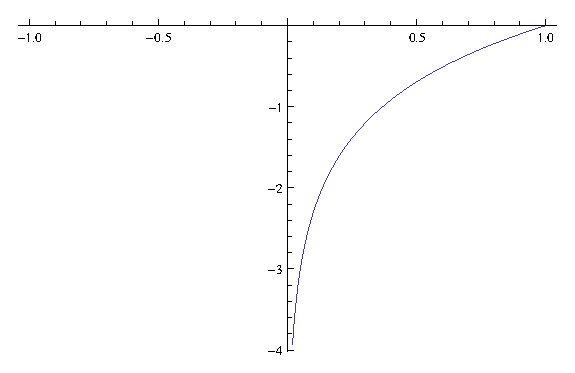
\includegraphics[width=0.4\textwidth]{continuous/transcend/natlog}
  \end{center}
  \caption{A plot of $f(x) =\ln x$.}
  \label{fig:natlog}
\end{figure}

\begin{defn}
  The \textbf{natural logarithm}\index{natural logarithm} is the function given by
  \begin{equation}
    \ln x = \int ^{x} _{1} \frac{1}{t} \ud t \text{,} \qquad x \in \mathbb{N}
  \end{equation}
\end{defn}
\begin{defn}
  The \textbf{number $e$} is that number in the domain of the natural logarithm satisfying
  \[ \ln{e}=1 \]
  It is roughly equal to
  \[2.7182818284590452353602874713526624977572470936999595\ldots\]
\end{defn}
\subsection{Algebraic Properties of the Natural Logarithm}

For any numbers $b>0$ and $x>0$, the natural logarithm satisfies the following rules:
\begin{table}[H]
    \begin{tabular}{p{3in}>\(p{3in}<\)}
      Product Rule      & \displaystyle{ \ln{bx}=\ln b + \ln x} \\\\
      Quotient Rule     & \displaystyle{ \ln{\frac{b}{x}}=\ln b - \ln x} \\ \\
      Reciprocal Rule   & \displaystyle{ \ln{\frac{1}{x}}=-\ln x} \\\\
      Power Rule        & \displaystyle{ \ln{x^r}=r \ln x \qquad \forall r \in \mathbb{R}}
    \end{tabular}
\end{table}
% \begin{equation}
% 	\ln{bx}=\ln b + \ln x
% \end{equation}
% \begin{equation}
% 	\ln{\frac{b}{x}}=\ln b - \ln x
% \end{equation}
% \begin{equation}
% 	\ln{\frac{1}{x}}=-\ln x
% \end{equation}
% \begin{equation}
% 	\forall r \in \mathbb{R} \quad \ln{x^r}=r \ln x
% \end{equation}

%The following table was sourced from \url{www.math.ualberta.ca/~apotapov/MATH115/ln-logs.pdf}:
\section{Logarithmic Identities}
\begin{align*}
  a^xa^y &=a^{x+y} & \log_a{(uv)}&=\log_a u+\log_a v \\
  (a^x)^y &= a^{xy} & \log_a{(u^y)} &= y\log_a u \\
  a^{-x} &= \frac{1}{a^x} & \log_a{\left(\frac{1}{u}\right)} &= -\log_a u \\
  \frac{a^x}{a^y} &= a^{x-y} & \log_a {\frac{u}{v}}&=\log_a u-\log_a v
\end{align*}

The number $e$ and its relationship to logarithms becomes especially important in integration,
where we manipulate its properties in calculus to solve equations and integrate functions we would not
otherwise be able to handle.

The inverse equations for $e^x$ and $\ln x$ are
\begin{equation}
  \forall (x>0)\big[e^{\ln x}=x\big]
  \label{eq:exinv1}
\end{equation}
\begin{equation}
  \forall x\big[\ln{(e^x)} =x\big]
  \label{eq:exinv2}
\end{equation}

The derivative of $e^x$ is very special, and it is
\begin{equation}
  \ddx e^x = e^x \ud x.
  \label{eq:ddxex}
\end{equation}


\section{Hyperbolic Functions}
Both \(\cos x\) and \(\sin x\) come from the formula for a circle.
\begin{equation}
  x^2 + y^2=r^2
  \label{eq:circle}
\end{equation}

But we can define other useful functions using the equation for a hyperbola.
\begin{equation}
  x^2-y^2=1
  \label{eq:hyperbola}
\end{equation}
Namely, \(\cosh x\) and \(\sinh x\).

In \ref{eq:hyperbola}, let \[ y \to \frac{e^x-e^{-x}}{2}\] to get \(\sinh x\).
Let \[ x \to \frac{e^x+e^{-x}}{2}\] to find \(\cosh x\).

We can prove that these still satisfy equation \ref{eq:hyperbola}:

\begin{proof}
  \begin{align*}
    1&=x^2-y^2 \\
    1&=\left( \frac{e^x+e^{-x}}{2} \right) - \left( \frac{e^x - e^{-x}}{2}
    \right)^2 \\
    1&=\frac{e^{2x}+2e^xe^{-x}+e^{-2x}}{4}-\frac{e^{2x}-2e^xe^{-x}+e^{-2x}}{4}
    \qedhere
  \end{align*}
\end{proof}

\chapter{Techniques of Integration}

\section{A Brief Table of Integrals}

\subsection{Basic Forms}

\begin{equation}
  \int k\,\ud x=kx+C \qquad \text{(any number \emph{k})}
\end{equation}
\begin{equation}
  \int x^n \, \ud x = \frac {x^{n+1}}{n+1}+C\,(n \neq -1)
\end{equation}
\begin{equation}
  \int \frac{\ud x}{x}=\ln{|x|}+C
\end{equation}
\begin{equation}
  \int e^x\, \ud x=e^x+C
\end{equation}
\begin{equation}
  \int a^x\, \ud x=\frac{a^x}{\ln a}+C \,(a>0,a\neq 1)
\end{equation}
\begin{equation}
  \int \sin x \, \ud x=-\cos x +C
\end{equation}
\begin{equation}
  \int \cos x \ud x=sin\,x+C
\end{equation}
\begin{equation}
  \int \sec^2x \ud x = \tan x + C
\end{equation}
\begin{equation}
  \int \csc^2 x \ud x = -cot\,x +C
\end{equation}
\begin{equation}
  \int \sec x \tan x \ud x = \sec x +C
\end{equation}
\begin{equation}
  \int \csc x \cot x \,dx = -\csc x +C
\end{equation}
\begin{equation}
  \int \cot x \ud x=\ln{|\sin x|}+C
\end{equation}
\begin{equation}
  \int \cosh x \ud x=\sinh x\,+C
\end{equation}
\begin{equation}
  \int \frac{\ud x}{a^2+x^2}=\frac{1}{a}\arctan{\frac{x}{a}}+C
\end{equation}
\begin{equation}
  \frac{\ud x}{\sqrt{a^2+x^2}}=\arcsin{\frac{x}{a}+C} \qquad (a > 0)
\end{equation}


\section{Integration by Parts}\index{integration by parts}
% rewrite this.
Integration by parts is used for simplifying integrals of the form
\[ \int f(x)g(x) \ud x \text{.} \]
It is useful when \(f\) can be differentiated repeatedly and $g$ can be integrated repeatedly without difficulty. The integrals
\[ \int x \cos x \ud x \quad \text{and} \quad \int x^2 e^x \ud x \]
are such integrals because $f(x)=x$ or $f(x)=x^2$ can be differentiated repeatedly to become zero, and $g(x)=\cos x$ or $g(x)=e^x$ can be integrated repeatedly without difficulty. Integration by parts also applies to integrals like
\[ \int \ln x \ud x \quad \text{and} \quad \int e^x \cos x \ud x \]
In the first case, $f(x)=\ln x$ is easy to differentiate and $g(x)=1$ easily integrates to $x$. In the second case, each part of the integrand appears again after repeated differentiation or integration.


\subsection{Integration By Parts Formula}

If $f$ and $g$ are differentiable functions of $x$, the Product Rule says that
$$ \frac{\ud}{\ud x} [f(x)g(x)]=f'(x)g(x)+f(x)g'(x) $$
In terms of indefinite integrals, this equation becomes
$$ \int \frac{\ud}{\ud x} [f(x)g(x)] \ud x=\int [f'(x)g(x)+f(x)g'(x)] \ud x $$
or
$$ \int \frac{\ud}{\ud x} [f(x)g(x)] \ud x=
\int f'(x)g(x) \ud x + \int f(x)g'(x) \ud x $$
Rearranging the terms of this last equation, we get
$$ \int f(x)g'(x) \ud x =
\int \frac{\ud}{\ud x}[f(x)g(x)]\ud x - \int f'(x)g(x) \ud x $$
Leading to the \textbf{integration by parts} formula
\begin{equation}
  \int f(x)g'(x)=f(x)g(x)-\int f'(x)g(x) \ud x
\end{equation}
Sometimes it is easier to remember the formula if we write it in differential form. Let $u=f(x)$ and $v=g(x)$. Then $\ud u=f'(x)\ud x$ and $\ud v=g'(x)\ud x$. Using the Substitution Rule, the \textbf{integration by parts} formula becomes
\begin{equation}
  \int u \ud v =  uv - \int v \ud u
  \label{equation:intbyparts}
\end{equation}

This formula expresses one integral, $\int u \ud v$, in terms of a second integral, $\int v \ud u$. With a proper choice of $u$ and $v$, the second integral may be easier to evaluate than the first.

\begin{ex}
  Integrate
  \[
    \int x \cos x \ud x.
    \]
    \begin{sol}
      We use integration by parts with
      \begin{align*}
        u&= x & \ud v &= \cos x \\
        \ud u &= \ud x & v &= \sin x
      \end{align*}
      So our integral becomes something we can integrate.
      \begin{align*}
        \int x \cos x \ud x &= x \sin x - \int \sin x \ud x \\
        &= x \sin x + \cos x +C
      \end{align*}
    \end{sol}
\end{ex}

% Rewrite this. Copied from textbook.
The goal of integration by parts is to go from an integral $\int u \ud v$ that we don't see how to evaluate to an integral $\int v \ud u$ that we can evaluate.
Generally, you choose $\ud v$ first to be as much of the integrand, including $\ud x$, as you can readily integrate; $u$ is the leftover part.
When finding $v$ from $\ud v$, any antiderivative will work and we usually pick the simplest one; no arbitrary constant of integration is needed in $v$ because it would simply cancel out on the right-hand side of \ref{equation:intbyparts}.

\begin{ex} A tough integration by parts problem.\footnote{Solved by Dr. James Martin, CNU Department of Mathematics. \url{http://math.cnu.edu/martin.htm}}
	\[ \int \frac{xe^{2x}}{(2x+1)^2}\ud x \]
  \begin{sol}
      We use integration by parts as follows:
      \begin{align*}
        u&=e^{2x} & \ud v&=\frac{x}{(2x+1)^2} \\
        \ud u &= 2e^{2x} & v &=\frac{1}{4+8x}+\frac{\ln{(1+2x)}}{4}
      \end{align*}
      To get:
      \begin{align*}
        \int \frac{xe^{2x}}{(2x+1)^2}\ud x
        =& \frac{e^{2x}}{4+8x}+\frac{e^{2x}\ln{|1+2x|}}{4}-\int 2e^{2x}\left[\frac{1}{4+8x}+\frac{\ln{(1+2x)}}{4}\right]\ud x \\
      \end{align*}
      Then we simplify the integrand.
      \begin{align*}
        \int \frac{xe^{2x}}{(2x+1)^2}\ud x =& \frac{e^{2x}}{4+8x}+\frac{e^{2x}\ln{|1+2x|}}{4}-\int \frac{2e^{2x}}{4+8x}\ud x-\frac{1}{2} \int e^{2x}\ln{|1+2x|}\ud x \\
        =& \frac{e^{2x}}{4+8x}+\frac{e^{2x}\ln{|1+2x|}}{4}-\frac{1}{2}\int \frac{e^{2x}}{1+2x}\ud x-\frac{1}{2} \int e^{2x}\ln{|1+2x|}\ud x
      \end{align*}
      We use integration by parts again on the second integral as follows:
      \begin{align*}
        u=&\ln{|1+2x|} & \ud v=&e^{2x} \\
        \ud u=&\frac{2}{1+2x}\ud x & v=& \frac{1}{2}e^{2x}
      \end{align*}
      \begin{align*}
        =& \frac{e^{2x}}{4+8x}+\frac{e^{2x}\ln{|1+2x|}}{4}
        -\frac{1}{2}\left[\frac{1}{2}e^{2x}\ln{|1+2x|}
          -\frac{1}{2} \int \frac{2e^{2x}}{1+2x} \ud x\right]
          -\frac{1}{2}\int \frac{e^{2x}}{1+2x}\ud x \\
          \intertext{We simplify our result, and all but one of the terms cancel:}
          =& \frac{e^{2x}}{4+8x}+\frac{e^{2x}\ln{|1+2x|}}{4}
          -\frac{1}{4}e^{2x}\ln{|1+2x|}
          + \frac{1}{2} \int \frac{e^{2x}}{1+2x} \ud x
          -\frac{1}{2}\int \frac{e^{2x}}{1+2x}\ud x \\
          =& \frac{e^{2x}}{4+8x}+\frac{e^{2x}\ln{|1+2x|}}{4}
          -\frac{e^{2x}\ln{|1+2x|}}{4}+C \\
          =& \frac{e^{2x}}{4+8x}+C
        \end{align*}
\end{sol}
\end{ex}
\begin{ex}
  Integrate
  \[\int\ln x \ud x.\]
  \begin{sol}
  Since $\int \ln x \ud x$ can be written as $\int \ln x \cdot 1 \ud x$, we can use integration by parts as follows:
  \begin{align*}
    u&=\ln x & \ud v &= \ud x \\
    \ud u &= \frac{\ud x }{x} & v&=x
  \end{align*}
  Which gives us the integral
  \begin{align*}
    \int\ln x \ud x &=
      x \ln x - \int  \frac{x \ud x}{x} \\
      &= x \ln x - \int \ud x \\
      &= x \ln x - x + C
    \end{align*}
  \end{sol}
\end{ex}

\subsection{Integration by Parts Cheat Sheet}
This is a set of guidlines\footnote{Proposed by Herbert Kasube of Bradley University.} advising whichever part of an integral comes first in this list should be assigned to $u$.
\begin{enumerate}
  \item Logarithms
  \item Inverse functions
  \item Algebraic
  \item Trigonometric
  \item Exponential
\end{enumerate}


\subsection{Reduction Formulas}
% probably rewrite this. I think I might have too much unoriginal material in this section.
Consider the integral
\begin{align*}
  I_n=&\int x^n e^{ax} \ud x
  \intertext{Integration by parts gives you}
  I_n=&x^n \frac{1}{a}e^{ax}-\int nx^{n-1}\frac{1}{a}e^{ax}\ud x \\
     =&\frac{1}{a}x^ne^{ax}-\frac{n}{a}\int x^{n-1}e^{ax}\ud x
\end{align*}
We haven't computed the integral. What we have done is derived the following \textbf{reduction formula}
\begin{equation}
  I_n=\frac{1}{a}x^ne^{ax}-\frac{n}{a}I_{n-1}
\end{equation}
which holds for all $n$.

For $n=0$ the reduction formula says
$$ I_0=\frac{1}{a}e^{ax} \to \int e^{ax}\ud x = \frac{1}{a}e^{ax}+C $$

When $n \neq 0$ the reduction formula tells us that we have to compute $I_{n-1}$ if we want to find $I_n$. The point of a reduction formula is that the same formula also applies to $I_{n-1}$, and $I_{n-1}$, etc. so that after repeated application of the formula we end up with $I_0$, an integral we know how to compute.\cite{freenotes}
\begin{ex}
  %[textbook: \#4/pg.441]
  Integrate
  \[ \int e^x \cos x \ud x \]
  \begin{sol}
    We use integration by parts with
    \begin{align*}
      u &= \cos x & \ud v &= e^x \ud x \\
      \ud u &= - \sin x \ud x & v &=e^x
    \end{align*}
    Which gives us the integral
    \begin{align*}
      \int e ^x \cos x \ud x &= e^x \cos x - \int -e^x \sin x \ud x \\
      &= e^x \cos x+ \int e^x \sin x \ud x \\
      \intertext{Now we use $u$-substitution with $u=e^x$ and $\ud u = e^x \ud x$.}
      &= e^x \cos x + \int \sin u \ud u \\
      &= e^x \cos x - \cos u +C \\
      &= e^x \cos x - \cos {e^x} +C
    \end{align*}
  \end{sol}
\end{ex}
\begin{ex}
  Integrate
  \[ \int (1-x)^{9}\ud x. \]
  \begin{sol}
    This is not an integration by parts problem.
    It is just a regular $u$-substitution and power rule problem.
    Let $u=1-x$ and $\ud u = -\ud x$.
    \begin{align*}
      \int (1-x)^9 \ud x &= -\int u ^9 \\
      &= -\frac{u^{10}}{10}+C\\
      &= -\frac{(1-x)^{10}}{10}+C
    \end{align*}
  \end{sol}
\end{ex}
\begin{ex}
  Integrate:
  \[
    \int 3x^2 \cos x^3 \ud x
    \]
  \begin{sol}
    Again, this is not an integration by parts problem.
    Because we can spot the derivative of $x^3$ clearly in the integrand,
    we can let $u=x^3$ and $\ud u = 3x^2 \ud x$.
    \begin{align*}
      \int 3x^2 \cos x^3 \ud x & = \int \cos u \ud u \\
      &= \sin u +C\\
      &= \sin {x^3}+C
    \end{align*}
  \end{sol}
\end{ex}
\begin{ex}
  Integrate
  \[
    \int x \cos x \ud x
    \]
    \begin{sol}
      Use integration by parts with
      \begin{align*}
        u &= x & \ud v &= \cos x \ud x \\
        \ud u &= \ud x & v &= \sin x
      \end{align*}
      Which gives us
      \begin{align*}
        \int x \cos x \ud x &= x \sin x - \int \sin x \ud x \\
        &= x \sin x + \cos x +C
      \end{align*}
    \end{sol}
\end{ex}
\begin{ex}
  Integrate
  \[
    \int x e^x \ud x
    \]
    \begin{sol}
      Use integration by parts with
      \begin{align*}
        u&=x & \ud v &= e^x \ud x \\
        \ud u &= \ud x & v &= e^x
      \end{align*}
      \begin{align*}
        \int x e^x \ud x &= x e^x -\int e^x \ud x \\
        &=x e^x -e^x +C
      \end{align*}
    \end{sol}
\end{ex}
\begin{ex}
  Integrate
  \[
    \int x \ln x \ud x
    \]
  \begin{sol}
    Use integration by parts with
    \begin{align*}
      u&= \ln x & \ud v &= x \ud x \\
      \ud u &= \frac{\ud x}{x} & v &= \frac{x^2}{2}
    \end{align*}
    Which gives us
    \begin{align*}
      \int x \ln x &= \frac{x^2 \ln x}{2}- \int \frac{x^2 \ud x}{2x} \\
      &= \frac{x^2 \ln x}{2}-\frac{1}{2} \int x \ud x \\
      &= \frac{x^2 \ln x}{2}-\frac{x^2}{4}+C
    \end{align*}
  \end{sol}
\end{ex}
\begin{ex}
  \[
    \int x e^{x^2} \ud x
    \]
    \begin{sol}
      This looks like an integration by parts problem at first, but again it is just a regular $u$-substitution problem.
      Let $u=x^2$ and $\ud u=2x\ud x$.
      \begin{align*}
        \int x e^{x^2} \ud x &= \frac{1}{2}e^u \ud u \\
        &= \frac{1}{2} e^u +C \\
        &= \frac{1}{2}e^{x^2} +C
      \end{align*}
    \end{sol}
\end{ex}
% PLEASE rewrite this section ASAP.
% Clean it up, add descriptions, put it in proper format, etc.
% This is priority #1 for now.
%
%  \begin{ex}
%    \[ \int x^3 e^{x^2} \ud x \]
%    Don't be discouraged if your first attempt at integration by parts fails.
%    \begin{align*}
%      u &= x^{3} & dv &= e^{x^{2}} \\
%      \ud u &= 3x^{2} \ud x & v &= \text{?}
%    \end{align*}
%    Just try again:
%    \begin{align*}
%      u &= x^2 & dv &= x e^{x^2} \ud x \\
%      \ud u &= 2x \ud x & v &= \frac{e^{x^2}}{2}
%    \end{align*}
%    \begin{align*}
%      \int x^3 e^{x^2} \ud x &=
%      \frac{x^2 e^{x^2}}{2} - \int \frac{2}{2} x e^{x^2} \ud x
%      =\frac {x^2 e^x}{2}- \frac {e^{x^2}}{2} + C \\
%      &=\frac{x^2 e^x-e^x}{2}+C
%    \end{align*}
%  \end{ex}
%  \begin{ex}
%    \[ \int e^x (x+1)^2 \ud x \]
%    Start with integration by parts:
%    \begin{align*}
%      u &= (x+1)^2 & \ud v &= e^x \ud x \\
%      \ud u &= 2(x+1)\ud x & v &= e^x
%    \end{align*}
%    \begin{align*}
%      \int e^x (x+1)^2 \ud x&=
%        e^x (x+1)^2 - \int e^x 2(x+1)\ud x \\
%      &=e^x (x+1)^2 - 2\int e^x (x+1)\ud x
%    \end{align*}
%    Saving this for later...
%    \begin{comment}
%    Then use integration by parts again:
%    \begin{align*}
%      u &= x+1 & \ud v &= e^x \ud x \\
%      \ud u &= \ud x & v &= e^x
%    \end{align*}
%    \begin{align*}
%      \int e^x (x+1)^2 \ud x&=
%        e^x (x+1)^2 - 2\left[e^x(x+1)-\int e^x \ud x \right] \\
%      &=e^x (x+1)^2 - 2[e^x(x+1)-e^x] + C \\
%      &=e^x (x+1)^2 - 2e^x(x+1)+2e^x + C\\
%      &=x^2e^x+e^x-2xe^x-2e^x+2e^x+C
%    \end{align*}
%    \end{comment}
%  \end{ex}
%  \begin{ex}
%    Another ``strange'' integral:
%    \[ \int \arcsin x \ud x \]
%  \end{ex}
%  \begin{ex}
%    \[ \int \sin^{-1}x \ud x \]
%    \begin{align*}
%      u &= \sin^{-1}x & \ud v&=\ud x\\
%      \ud u &= \frac {1}{\sqrt{1-x^2}} \ud x & v &= x
%    \end{align*}
%    \begin{align*}
%      \int \sin^{-1}x \ud x &=
%      x \sin^{-1}x - \underbrace{\int \frac {x}{\sqrt{1-x^{2}}} \ud x}_{\lets u = 1-x^{2}}=x \sin^{-1}x-\frac{1}{2} \int \frac{\ud u}{\sqrt{u}} \\
%      &=x \sin^{-1}x+\frac{1}{2} \int u^{-1/2}\ud u=x sin^{-1}x+\sqrt u +C \\
%      &=x \sin^{-1}x+\sqrt{1-x^{2}} +C
%    \end{align*}
%  \end{ex}
%  \begin{ex}
%    \[ \int 4x e^{4x} \ud x \]
%    \begin{sol}
%    We use integration by parts with
%    \begin{align*}
%      u&=x & \ud v&=e^{4x}\ud x \\
%      \ud u &=\ud x & v &=\frac{1}{4}e^{4x}
%  	\end{align*}
%  	\begin{align*}
%  	  \frac{1}{x^4+2x^2+1}
%  	    =&4\left[x \cdot \frac{1}{4}e^{4x}-\int 1 \cdot \frac{1}{4} e^{4x} \ud x\right] \\
%  	    =&4\left[x \cdot \frac{1}{4}e^{4x}-\frac{1}{4}\int e^{4x} \ud x\right] \\
%  	    =& x e^{4x}-\frac{1}{4}e^{4x} + C
%    \end{align*}
%  \end{sol}
%  \end{ex}
%
%  % \begin{homework}
%  % pg. 489 odd 1-7, pg. 441 odd 1-23, pg. 441 6, 8, 35, 39.
%  % \end{homework}
%
%  \begin{ex}[\#23/pg.441]
%    \[ \int e^{2x}\cos{3x}\ud x \]
%    \begin{align*}
%      u &= \cos{3x} & \ud v&=e^{2x}\ud x\\
%      \ud u &= -3\sin{3x}\ud x & v&=\frac{1}{2}e^{2x}
%    \end{align*}
%    \begin{align*}
%      \int e^{2x}\cos{3x}\ud x &=
%        \frac{1}{2}e^{2x}\cos{3x}+\frac{3}{2}\int e^{2x}\sin{3x}\ud x \\
%      &=\frac{1}{2}e^{2x}\cos{3x}+\frac{3}{2}
%        \left[\frac{1}{2}e^{2x}\sin{3x}-\frac{3}{2}\int e^{2x}\cos{3x}\ud x \right]\ \\
%      \to\frac{4}{4}\int e^{2x}\cos{3x}\ud x
%        &=\frac{1}{2}e^{2x}\cos{3x}+\frac{3}{4}e^{2x}\sin{3x}-\frac{9}{4}\int e^{2x}\cos{3x}\ud x \\
%      \frac{13}{4}\int e^{2x}\cos{3x}\ud x
%        &=\frac{1}{2}e^{2x}\cos{3x}+\frac{3}{4}e^{2x}\sin{3x}+C \\
%      13\int e^{2x}\cos{3x}\ud x
%        &=2e^{2x}\cos{3x}+3e^{2x}\sin{3x}+C \\
%      \int e^{2x}\cos{3x}\ud x
%        &=\frac{2}{13}e^{2x}\cos{3x}+\frac{3}{13}e^{2x}\sin{3x}+C \\
%      &=\frac{e^{2x}}{13}\left[2\cos{3x}+3\sin{3x}\right]+C
%    \end{align*}
%    % Old in-class garbage:
%    % $$\frac{1}{2}cos(3x)e^{2x}+\frac{3}{2}\int e^{2x}sin(3x)\ud x \frac{1}{2}cos(3x)e^{2x}+\frac{3/2} (\frac{1}{2}e^{2x}sin(3x)-\frac{3}{2}\int e^{2x}cos(3x)\ud x)
%  \end{ex}
%  \begin{ex}
%    Integrate
%    \[ \int x^2\cos{3x}\ud x \]
%    \begin{sol}
%      Use integration by parts.
%      \begin{align*}
%        u&=x^2 && \ud v=\cos{3x}\ud x \\
%        \ud u=&2x\ud x && v=\frac{1}{3}\sin{3x}
%      \end{align*}
%      \begin{align*}
%        \int x^2\cos{3x}\ud x
%        =nt^{a}_{-\infty} f(x) \ud x
%            + \int^{\infty}_{a} f(x) \ud x& \frac{1}{3}x^2\sin{3x}-\frac{2}{3}\int x \sin{3x} \ud x \\
%        \intertext{Now use integration by parts again}
%        =& \frac{1}{3}x^2\sin{3x}-\frac{2}{3} \left( \frac{-x}{3}\cos{3x}+\frac{1}{3}\int\cos{3x}\ud x \right)\\
%        =& \frac{1}{3}x^2\sin{3x}+\frac{2}{9}x\cos{3x}-\frac{2}{27}\sin{3x}+C
%      \end{align*}
%    \end{sol}
%  \end{ex}
%  \begin{ex}
%    Integrate
%    \[ \int \frac{x}{\sqrt{x+3}} \]
%    \begin{sol}
%    Use integration by parts with
%    \begin{align*}
%      u&=x  & \ud v&=\frac{\ud x}{\sqrt{x+3}} \\
%      \ud u&=\ud x & v &=2\sqrt{x+3}
%    \end{align*}
%    \begin{align*}
%      \int \frac{x}{\sqrt{x+3}} =& 2x\sqrt{x+3}-\int 2\sqrt{x+3}\ud x \\
%      =& 2x \sqrt{x+3}-\frac{4}{3}(x+3)^{3/2}+C
%    \end{align*}
%  \end{sol}
%  \end{ex}
%  \begin{ex}
%    Integrate
%    \[\sin^{-1}{3x}\ud x\]
%    \begin{sol}
%      We use integration by parts with
%      \begin{align*}
%        u&=\arcsin{3x} & \ud v &= \ud x \\
%        \ud u &=\frac{3}{\sqrt{1-9x^2}}\ud x & v&=x
%      \end{align*}
%      \begin{align*}
%        \arcsin{3x}\ud x
%        =&x\arcsin{3x}-\int \frac{3x \ud x}{\sqrt{1-9x^2}} \\
%        =&x\arcsin{3x}+\frac{1}{3}\sqrt{1-9x^2}+C
%      \end{align*}
%    \end{sol}
%  \end{ex}


\section{Trigonometric Integrals}

Trigonometric integrals involve algebraic combinations of the six basic trigonometric functions. In principle, we can always express such integrals in terms of sines and cosines, but it is often simpler to work with other functions, as in the integral
$$ \int sec^2 x \ud x = \tan x + C $$
The general idea is to use identities to transform the integrals we have to find into integrals that are easier to work with.

We begin with integrals of the form:
$$ \int \sin^mx\cos^nx\ud x $$
where $m$ and $n$ are nonnegative integers (positive or zero). We can divide the appropriate substitution into three cases according to $m$ and $n$ being odd or even.
\begin{enumerate}
  \item If \textbf{$m$ is odd}, we write $m$ as $2k+1$ and use the identity $\sin^2x=1-\cos^2x$ to obtain
  $$sin^mx=sin^{2k+1}x=(sin^2x)^k\sin x=(1-\cos^2x)^k\sin x $$
  Then we combine the single $\sin x$ with $\ud x$ in the integral and set $\sin x \ud x$ equal to $-\ud (\cos x)$.
  \item If \textbf{$m$ is even and $n$ is odd} in $\int \sin^mx\cos^nx \ud x$, we write $n$ as $2k+1$ and use the identity $\cos^2x=1-\sin^2x$ to obtain
  $$ \cos^nx=\cos^{2k+1}x=(\cos^2x)^k\cos x=(1-\sin^2x)^k\cos x $$
  We then combine the single $\cos x$ with $\ud x$ and set $\cos x \ud x$ equal to $d(\sin x)$.
  \item If \textbf{both $m$ and $n$ are even} in $\int \sin^mx\cos^nx\ud x$, we subsitute
  \begin{align*}
    &\sin^2x=\frac{1-\cos{2x}}{2}
    &\cos^2x=\frac{1+\cos{2x}}{2}
  \end{align*}
  to reduce the integrand to one in lower powers of $\cos{2x}$.
\end{enumerate}

We can also use trigonometric identities to eliminate square roots in integrals:
\begin{ex}
  \[ \int^{\frac{\pi}{4}}_{0} \sqrt{1+\cos{4x}}\ud x \]
  To eliminate the square root, we use the identity
  \[ \cos^2 \theta = \frac{1+\cos{2 \theta}}{2} \]
  With $\theta=2x$, this becomes:
  \[ 1+\cos{4x}=2\cos^2{2x} \]
  Therefore,
  \begin{align*}
    \int^{\frac{\pi}{4}}_{0} \sqrt{1+\cos{4x}}\ud x&= \int^{\frac{\pi}{4}}_{0} \sqrt{2 \cos^2{2x}} \ud x = \int^{\frac{\pi}{4}}_{0} \sqrt2 \sqrt{\cos^2{2x}} \\
    &= \sqrt2 \int^{\frac{\pi}{4}}_{0} |\cos{2x}|\ud x = \sqrt2 \int^{\frac{\pi}{4}}_{0} \cos{2x}\ud x \\
    &= \sqrt2 \left[\frac{\sin{2x}}{2}\right]^{\frac{\pi}{4}}_{0} = \frac{\sqrt2}{2}[1-0] \\
    &= \frac{\sqrt2}{2}
  \end{align*}
\end{ex}


\subsection{Examples}
\begin{comment}
  I don't like how this is structured.
  \begin{itemize}
      \item $ \int tan^{\text{power}}x \, sec^{\text{even}}x\ud x$
      \item $ \int \underbrace{sin^{\text{power}x} \, cos^{\text{power}}x \ud x}_{\text{except where both are even}} $
      \item $ \int cot^{\text{power}x} \, csc^{\text{even}}x \ud x $
      \item $ \int sin(mx) \,  sin(nx) \ud x = \int \frac{1}{2}(cos(m-n)x-cos(m+n)x)$
      \item $ \int cos(mx) \,  cos(nx) \ud x = \int \frac{1}{2}(cos(m-n)x-cos(m+n)x)$
  \end{itemize}
\end{comment}

\begin{ex}
  \[ \int \sin^7x \cos^2x \ud x \]
  \begin{sol}
  \begin{align*}
    \int \sin^7x \cos^2x \ud x &=
      \int \sin^6x \cos^2x \sin x \ud x \\
    &=(\sin^2x)^3\cos^2x\sin x\ud x \\
    \intertext{because $\sin^2x=1-\cos^2x$}
    &=(1-\cos^2x)^3 \cos^2x\sin x \ud x
    \intertext{let $u=\cos x$ and $\ud u=-\sin x$.}
    &=-\int(1-u^2)^3u^2\ud u \\
    &=-\int (1-u^2)(1-u^2)(1-u^2)u^2\ud u \\
    &=-\int(1-2u^2+u^4)(1-u^2)u^2 \ud u \\
    &=-\int(u^2-2u^4+u^6-u^4+2u^6-u^8)\ud u \\
    &=\frac{-u^3}{3}+\frac{2u^5}{5}-\frac{u^7}{7}+\frac{u^5}{5}-\frac{2u^7}{7}+\frac{u^9}{9}+C \\
    &=\frac{-\cos^3x}{3}+\frac{2\cos^5x}{5}-\frac{\cos^7x}{7}+\frac{\cos^5x}{5}-\frac{2\cos^7x}{7}+\frac{\cos^9x}{9}+C
  \end{align*}
\end{sol}
\end{ex}
\begin{ex}
	\[ \int \cos^7x \sin^2x \ud x \]
	\begin{sol}
	\begin{align*}
		\int \cos^7x \sin^2x \ud x &=
		  \int \cos^6x \sin^2x \cos x \ud x
		\intertext{Because $\cos^2x=1-\sin^2x$:}
		&=\int (1-\sin^2x)^3\sin^2x\cos x \ud x \\
		\intertext{Now let $u=\sin x$ and $\ud u=\cos x \ud x$.}
		&= \int(1-u^2)^3u^2 \ud u \\
		&= \int (u^2-2u^4+u^6-u^4+2u^6-u^8) \ud u \\
		&= \frac{u^3}{3}-\frac{2u^5}{5}+\frac{u^7}{7}-\frac{u^5}{5}+\frac{2u^7}{7}-\frac{u^9}{9}+C \\
		&= \frac{\sin^3x}{3}-\frac{2\sin^5x}{5}+\frac{\sin^7x}{7}-\frac{\sin^5x}{5}+\frac{2\sin^7x}{7}-\frac{\sin^9x}{9}+C \\
		&= \frac{\sin^3x}{3}-\frac{\sin^5x}{5}+\frac{3\sin^7x}{7}-\frac{\sin^9x}{9}+C
	\end{align*}
\end{sol}
\end{ex}
\begin{ex}
	\[\int \sin^{15}x\ud x \]
	\begin{sol}
	\begin{align*}
		\int \sin^{15}x\ud x&=\int sin^{14}x \sin x \ud x =\int (\sin^2x)^7 \sin x \ud x \\
	  &=\int (1-\cos^2x)^7 \sin x \ud x
	  \intertext{Let $u=\cos x$ and $\ud u=-\sin x \ud x$.}
	  &=-\int (1-u^2)^7 \ud u =-\int \ud u + \int u^{14} \ud u=-u+\frac{u^{15}}{15}+C \\
	-  &=-\cos x + \frac{\cos^{15}x}{15}+C
	\end{align*}
\end{sol}
\end{ex}
\begin{ex}
  \[ \int \sin^2x \cos^2x \ud x \]
  \begin{sol}
    Remembering our power reduction identities from \eqref{eq:cossqq} and \eqref{eq:sinsqq}:
  \begin{align*}
	  \int \sin^2x \cos^2x \ud x &=\int \frac{1-\cos{2x}}{2} \cdot \frac{1+\cos{2x}}{2} \ud x =\frac{1}{4} \int (1-\cos^2{2x})\ud x \\
	  &= \frac{1}{4} \int \left(\frac{2}{2}-\frac{1+\cos{4x}}{2}\right)\ud x
	  =\frac{1}{4} \int \left(\frac{2-(1+\cos{4x})}{2}\right)\ud x \\
	  &=\frac{1}{4} \int \left(\frac{1-\cos{4x})}{2}\right)\ud x
	  =\frac{1}{8}\int 1-\cos{4x}\ud x \\
	  &=\frac{1}{8}\int \ud x - \frac{1}{8} \int \cos{4x}\ud x \\
	  &=\frac{x}{8}-\frac{1}{32}\sin{4x}+C
	\end{align*}
\end{sol}
\end{ex}
\begin{ex}
	\[ \int \tan^6x \sec^4x \ud x\]
	\begin{sol}
	\begin{align*}
		\int \tan^6x \sec^4x \ud x&=\int \tan^6x \sec^2x \sec^2x \ud x
		\intertext{Remembering that $\sec^2x=1+\tan^2x$:}
		&=\int \tan^6x (1+\tan^2x) \sec^2x \ud x
		\intertext{Now, letting $u=\tan x$ and $\ud u=\sec^2x\ud x$:}
		&= \int u^6(1+u^2)\ud u
		= \int u^6\ud u + \int u^8\ud u
		=\frac{u^7}{7}+\frac{u9}{9}+C \\
		&=\frac{\tan^7x}{7}+\frac{\tan^9x}{9}+C
	\end{align*}
\end{sol}
\end{ex}
\begin{ex}
  $$ \int cot^{8}x \, csc^{4}x \ud x $$
\end{ex}

% \begin{homework}
% Read section 8.2 and solve pg. 448 1-12,13,15,33,37,38,45,47,50,51,53,55,63,65,67
% \end{homework}


\section{Trigonometric Substitution}

\textbf{Trigonometric substitution} is the substitution of trigonometric functions for other expressions. One may use the trigonometric identities to simplify certain integrals containing radical expressions.

There are two important trig identities for us to know in this section:
\[ 1-sin^{2}\theta=cos^{2}\theta \]
\[ 1+tan^{2}\theta=sec^{2}\theta \]

We will find trigonometric substitution useful for problems that look this:

\[ \int \frac{dx} {x \sqrt{x^{2}-4}} \]

For integrands with $ \sqrt{x^{2}-a^{2}}$, $\lets x=a\sec \theta$ and let $\ud x = a \sec \theta \tan \theta \ud \theta $.
\begin{figure}[H]
  \begin{center}
    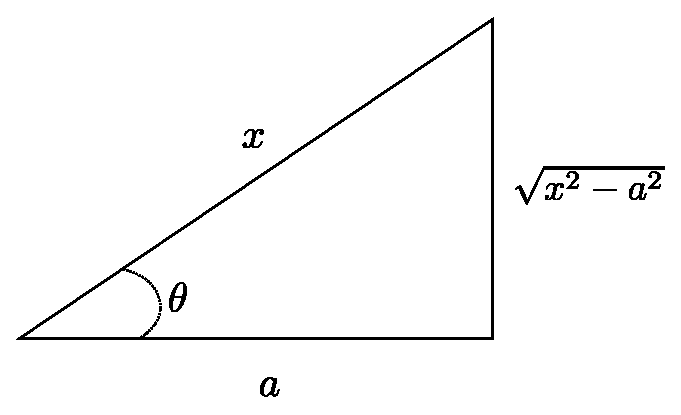
\includegraphics[width=0.4\textwidth]{continuous/integration/asectheta.eps}
  \end{center}
\end{figure}
For integrands with $\sqrt{a^2-x^2}$, let $x=a \sin \theta$ and $\ud x = a \cos \theta \ud \theta$.
\begin{figure}[H]
  \begin{center}
    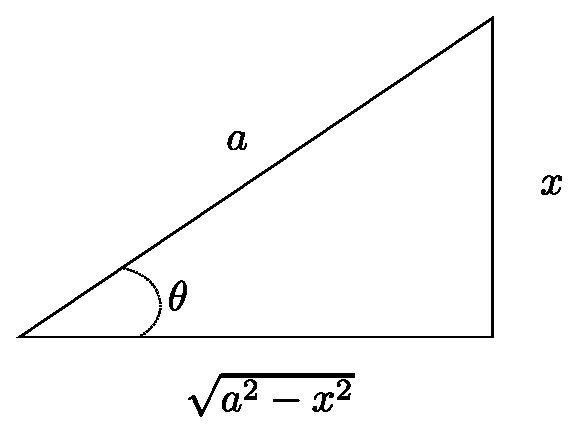
\includegraphics[width=0.4\textwidth]{continuous/integration/asintheta.eps}
  \end{center}
\end{figure}
For integrands with $ \sqrt{x^2+a^2}$, let $x = a \tan \theta$ and $\ud x = \sec^2 \theta \ud \theta$.
\begin{figure}[H]
  \begin{center}
    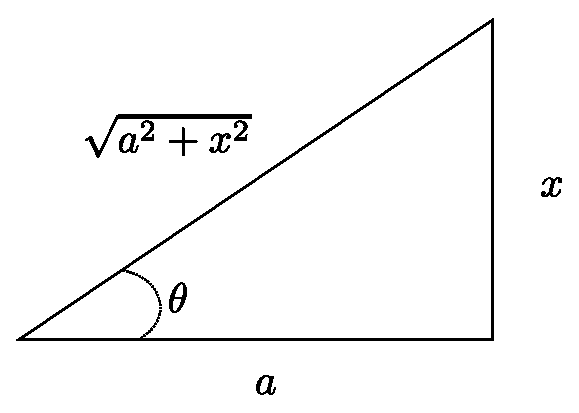
\includegraphics[width=0.4\textwidth]{continuous/integration/atantheta.eps}
  \end{center}
\end{figure}

\begin{ex}
  Integrate
  \[ \int \frac{\ud x}{x \sqrt {x^2 -4}} \]
  \begin{sol}
    Let $x=2 \sec \theta$ and $\ud x = 2 \sec \theta \tan \theta \ud \theta$.
    \begin{align*}
      \int \frac{\ud x}{x \sqrt {x^2 -4}}
      &= \int \frac{2 \sec \theta \tan \theta \ud \theta}{2 \sec \theta \sqrt{4\sec^2 \theta -4}} \\
      &= \int\frac{tan \theta \ud \theta}{\sqrt{4 \sec^2 \theta -4}} \\
      \intertext{Now we use the trigonometric identity $1+\tan^2\theta=\sec^2\theta$.}
      &= \int \frac{\tan\theta\ud\theta}{\sqrt{4(1+\tan^2\theta)-4}}\\
      &= \int \frac{\tan\theta\ud\theta}{\sqrt{4\tan^2\theta}}\\
      &= \int\frac{\tan\theta\ud\theta}{2\tan\theta}\\
      &= \int \frac{1}{2}\ud\theta \\
      &= \frac{1}{2}\theta+C\\
      \intertext{Now we draw a triangle, using the numbers from our original substitution:}
      % add a picture
      &=\frac{1}{2}\arcsec{\frac{x}{2}} +C
    \end{align*}
    \begin{figure}[H]
      \begin{center}
        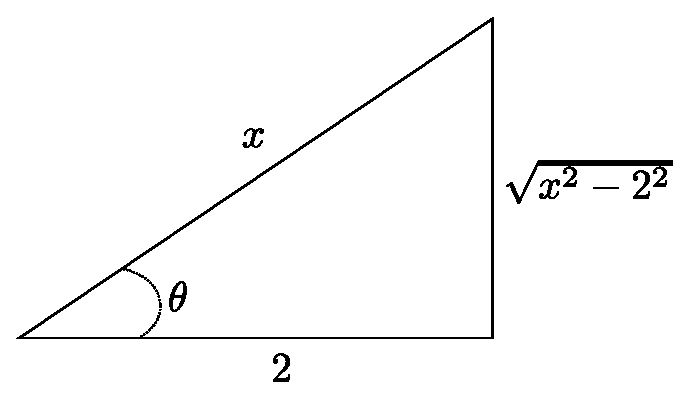
\includegraphics[width=0.4\textwidth]{continuous/integration/secexample.eps}
      \end{center}
    \end{figure}
  \end{sol}
\end{ex}
% \begin{ex}
%   \[ \int \frac{dx} {x \sqrt{x^{2}-4}} \]
%   \begin{sol}
%   \begin{align*}
%     \lets x&=2\sec \theta & \lets dx &= 2 \sec \theta \tan \theta \ud \theta
%   \end{align*}
%   \begin{align*}
% 	  \int \frac{\ud x} {x \sqrt{x^2-4}}
% 	  =&\int \frac{2 \sec \theta \tan \theta \ud \theta}{2 \sec \theta \sqrt{4\sec^2\theta-4}} \\
% 	  =&\int \frac{\tan \theta \ud \theta}{\sqrt{4\sec^2 \theta-4}} \\
% 	  =&\int \frac{\tan \theta}{2 \tan \theta} \ud \theta
% 	  = \frac {1}{2} \theta + C \\
%   \end{align*}
% This is unfinished, we still need to solve for $\theta$.
% \end{sol}
% \end{ex}
\begin{ex}
  \[ \int \frac{\ud x}{\sqrt{1-x^{2}}} = \sin^{-1}x+C \]
\end{ex}
\begin{ex}
  \[ \int \frac{2x}{\sqrt{1-x^2}}dx \]
  \begin{sol}

  \[ \text{let} u = 1-x^{2} \ldots \]
\end{sol}
\end{ex}
\begin{ex}
  \[ \int x^{3} \sqrt {4-x^2} \ud x \]
  \begin{sol} Although perhaps solvable using integration by parts, we will use trigonometric substitution.
  \begin{align*}
    \lets  x &= 2 \sin{\theta} \\ \lets \ud x &= 2\cos \theta \ud \theta
  \end{align*}
  \begin{align*}
    \int x^{3} \sqrt {4-x^2} \ud x
    =&\int 8\sin^3 \theta \, 2\cos\theta \, 2\cos\theta \, \ud\theta
   =32 \int \sin^{3}\theta\cos^{2} \theta \ud\theta \\
   =& 32 \int \sin^{2}\theta\cos^{2} \theta\sin \theta \ud\theta \\
   =& 32 \int (1-\cos^{2}\theta) \cos^{2} \theta\sin \theta \ud\theta \\
   \intertext{Let $u=\cos\theta$ and $\ud u = -\sin \theta \ud \theta$.}
   =&-32 \int (1-u^{2})\,u^{2}\ud u \\
   =&\frac {-32u^3}{3}+\frac{32u^5}{5}+C \\
   =&\frac{-32\cos^{2}\theta}{3}+\frac{32\cos^{5}\theta}{5}+C \\
   =&\frac {-32}{3} \left(\frac{\sqrt{4-x^2}}{2}\right)+\frac {32}{5} \left(\frac{\sqrt{4-x^2}}{2}\right)^5+C \\
 \end{align*}
 \end{sol}
\end{ex}

% \begin{homework}
%   Read Section 8.3.
% \end{homework}

\begin{ex}
  \[ \int \sqrt{x^2+6x} \ud x \]
  \begin{sol}
    \begin{align*}
      \int \sqrt{x^2+6x} \ud x =&\int \sqrt{x^2+6x+9-9}\ud x
      =\int \sqrt{(x+3)^2-9}\ud x \\
      \intertext{Now let $x+3=3\sec\theta$ and $\ud x=3\sec\theta \tan\theta \ud\theta$.}
      =& 3 \int \sqrt{9\sec^2\theta-9}\sec\theta \tan\theta \ud \theta \\
      =& 9 \int \tan^2\theta\sec\theta\ud\theta
  \end{align*}
\end{sol}
\end{ex}
\begin{ex}
  Integrate
    \[ \int \frac{1}{\sqrt{x^2+2x+5}}\ud x \]
  \begin{sol}
    \begin{align*}
      \int \frac{1}{\sqrt{x^2+2x+5}}\ud x
      =& \int \frac{1}{\sqrt{x^2+2x+1+4}} \\
      =& \int \frac{1}{\sqrt{(x+1)^2+4}} \\
      \intertext{Let $u=x+1$ and $\ud u=\ud x$.}
      =& \int \frac{\ud u}{\sqrt{u^2+4}} \\
      =& \arcsin \frac{x+1}{4}+C
    \end{align*}
  \end{sol}
\end{ex}


\section{Partial Fraction Decomposition}

A rational function $P(x)/Q(x)$ can be rewritten using what is known as partial fraction decomposition. This procedure often allows integration to be performed on each term separately by inspection. For each factor of $Q(x)$ the form $(a\,x+b)^m$:

\begin{equation}
  \frac{A_1}{a\,x+b}+\frac{A_2}{(a\,x+b)^2}+\ldots+\frac{A_m}{(a\,x+b)^m}
\end{equation}

For each factor of the form $(a\,x^2+b\,x+c)^m$ introduce terms:

\begin{equation}
  \frac{A_1\,x+B_1}{a\,x^2+b\,x+c}+\frac{A_2\,x+B_2}{(a\,x^2+b\,x+c)^2}+\ldots+\frac{A_m\,x+B_m}{(a\,x^2+b\,x+c)^m}
\end{equation}

Then write:

\begin{equation}
  \frac{P(x)}{Q(x)}=\frac{A_1}{a\,x+b}+\ldots+\frac{A_2\,x+B_2}{(a\,x^2+b\,x+c)^2}+\ldots
\end{equation}

And solve for $A_i$s and $B_i$s.


\subsection{Repeated Linear/Quadratic Den. Factors}

\begin{align*}
  \frac {\cdots}{\underbrace{(x^2+3)^2}_\text{quadratic} \, \underbrace{(x+1)}_\text{linear} \, \underbrace{(x^2+x+4)}_\text{quadratic}}
  &=\frac {Ax+B}{(x^2+3)^2} + \frac{Cx+D}{(x^2+3)^1} + \frac {E}{x+1} + \frac {Fx+G}{x^2+x+4}
\end{align*}

\begin{align*}
  \frac {\cdots}{(x^2-2x+1)(x^2-4x+4)}
  &=\frac {\cdots}{(x-1)^2(x-2)^2} \\
  &=\frac{A}{(x-1)^2}+\frac{B}{x-1}+\frac{C}{(x-2)^2}+\frac{D}{x-2}
\end{align*}

\subsection{Determining A,B,C, \dots}

Multiply the denominator by both sides of the new equation:
\[ {denominator}*\left[\frac{x^3+2x^2+x+8}{(x^2+4)^2}\right]=\left[\frac{Ax+B}{(x^2+4)^2}+\frac{Cx+D}{(x^2+4)^1}\right]*{denominator} \]

Now solve for \(A\), \(B\), and \(C\).

\begin{align*}
  x^3+2x^2+x+8 &= (Ax+B)+\,(Cx+D)(x^2+4)\\
  x^3+2x^2+x+8 &= (Ax+B)+Cx^3+4Cx+Dx^2+4D
\end{align*}

Now:
\begin{table}[H]
  \centering
  \begin{tabular}{r|l}
    \(x^2\) terms & \( 2=D \) \\
    \(x\) terms & \( 1 = A + 4C  \) \\
    const terms & \( 8 = B + 4D \)
  \end{tabular}
\end{table}

\subsection{Factoring}

\begin{equation}
  (F)^3+(L)^3=(F+L)(F^2-FL+L^2)
\end{equation}
\begin{equation}
  (F)^3-(L)^3=(F-L)(F^2+FL+L^2)
\end{equation}
Note: you cannot factor a sum of perfect squares.
\begin{remark} When factoring quadratics, consider the discriminant (from the quadratic formula at \ref{app:eq:quadratic}):
  \begin{align*}
    &10x^2-x-2 \\
    &b^2-4ac \\
    &(-1)^2-4(10)(-2)
  \end{align*}
\end{remark}

% \begin{homework} From \emph{Thomas' Calculus}, solve
%
%   \begin{tabular}{llr}
%     page & problems & sols \\ \hline
%     475 & 25 \\ & 27 (b) \\ & 32 \\
%     492 & 70 & $\frac{-x^2}{2}-\frac{3}{2}\ln{|x+2|}-\frac{5}{2}ln{|x-2|}$ \\
%     & 72 & ($\sin^1{x+1}$) \\
%     & 75 \\
%     & 75 & $\frac{x^2}{2}+2x+3ln{|x-1|}-\frac{1}{x-1}$ \\
%     & 79 \\ &83\\&85\\&86&$\frac{x^2-1}{2}e^{x^2}$\\&87\\&88&$\frac{-\tan^{-1}x}{x}+\ln{|x|}-\ln{\sqrt{|1+x^2}|}$\\&99\\&101\\
%   \end{tabular}
% \end{homework}


% \section{Test Review}
% \begin{comment}
% \begin{ex}
%   $$ \int cot^3 (2x)\ud x $$
%   $$ \int (csc^2 2x -1) \, cot2x \ud x $$
%   $$ \int csc^2 2x\, cot \, 2x \ud x - \int \frac {cos\,2x}{sin\,2x}\ud x $$
%   $$ \text {abandoned ...} $$
% \end{ex}
% \end{comment}
% %\begin{ex}
% %  Integrate \[ \int \sqrt{16-9x^2} \ud x \]
% %  \begin{sol}
% %  Factor out a $9$.
% %  \begin{align*}
% %    \int \sqrt{16-9x^2} \ud x
% %    =& \int \sqrt{9\left(\frac{16}{9}-x^2\right)} \ud x
% %    =3 \int \sqrt{\frac{16}{9}-x^2} \ud x \\
% %    \intertext{Let $x= \frac{4}{3}\sin \theta$ and $\ud x = \frac{4}{3}\cos \theta \ud \theta$.}
% %    =& 3 \int \sqrt{\frac{16}{9}-\left( \frac{4}{3}\sin\theta \right)^2}\,\frac{4}{3}\cos\theta\ud\theta \\
% %    =& 3 \int \sqrt{\frac{16}{9}-\frac{16}{9}\sin^2\theta}\,\frac{4}{3}\cos\theta\ud\theta \\
% %    =& 3 \int \frac{4}{3}\sqrt{1-\sin^2 \theta} \,\frac{4}{3}\cos\theta\ud\theta \\
% %    =& \frac{16}{3} \int \sqrt{\cos^2\theta}\cos\theta\ud\theta \\
% %    =& \frac{16}{3} \int \cos^2\theta\ud\theta
% %  \end{align*}
% %  \center{[Incomplete. See comments for details.]}
% %\end{sol}
% %\end{ex}
% %\begin{ex}
% %  $$ \int \sqrt{16-9x^2} \ud x $$
% %  $$ \int \sqrt{9\frac{16}{9}-x^2}\ud x $$
% %  $$ \text {try } x = \frac{4}{3}\sin \, \theta $$
% %  $$ dx = \frac{4}{3}cos\,\theta \, \ud \theta $$
% %  $$ 3 \int \sqrt{\frac{16}{9}-x^2}\ud x $$
% %  $$ 3 \int \sqrt{\frac{16}{9}-\frac{16}{9}sin^2 \, \theta } \, \frac{4}{3}cos\,\theta \, d\theta $$
% %  $$ 3 \int \frac {4}{3} \sqrt{cos^2 \, \theta } \frac{4}{3} cos\,\theta\,d\theta $$
% %  $$ \frac{16}{3} \int cos^2 \theta \, d \theta $$
% %  $$ \frac{16}{3}\left[\frac{\theta}{2}+\frac{sin\,2\theta}{4}\right] $$
% %  $$ \theta = sin^{-1}\,\frac{3x}{4} $$
% %  $$ \frac{16}{3}\left[\frac{sin^{-1}\,\frac{3x}{4}}{2}+\frac{sin\,2(sin^{-1}\,\frac{3x}{4})}{4}\right] $$
% %\end{ex}

\subsection{Examples}

\begin{ex}
  \begin{align*}
    \frac{x+3}{x^2-3x+2}
   =&\frac{x+3}{(x-2)(x-1)} \\
   =&\frac{A}{x-2}+\frac {B}{x-1}
  \end{align*}
\end{ex}
\begin{ex}
  \begin{align*}
    \frac {x+3} {x^4+3x^3+6x^2+12x+8}
    =&\frac {x+3} {(x^2+4)(x+1)(x+2)} \\
    =&\frac{A}{x+1}+\frac{b}{x+2}+\frac{Cx+D}{x^2+4}
  \end{align*}
\end{ex}
\begin{ex}
  \begin{align*}
    \frac{x+3}{x^4+5x^2+4}
    =&\frac{x+3}{(x^2+4)(x^2+1)}\\
    =&\frac{Ax+B}{x^2+4}+\frac{Cx+D}{x^2+1}
  \end{align*}
\end{ex}
\begin{ex}
  \begin{align*}
    \frac{1}{x^2-1}
    =&\frac{1}{(x-1)(x-1)} \\
    =&\frac{A}{x+1}+\frac{B}{x-1}
  \end{align*}
\end{ex}
\begin{ex}
  \begin{align*}
    \frac{1}{x^2-x}
     =&\frac{1}{x(x-1)} \\
     =&\frac{A}{x}+\frac{B}{x-1}
  \end{align*}
\end{ex}

\begin{ex}
  \begin{align*}
   \frac {9x^2+7x-4}{x^3-3x^2-4x} \\
   \frac {9x^2+7x-4}{x(x^2-3x-4)} \\
   \frac {9x^2+7x-4}{x(x-4)(x+1)} \\
   \frac{A}{x}+\frac{B}{x-4}+\frac{C}{x+1}
  \end{align*}
\end{ex}
\begin{ex}
  \begin{align*}
   \frac {x+3}{x^2-4} \neq \frac {A}{x+2} + \frac {B}{x-2} \\
   \frac {x+3}{x^2-4} = \frac {x^3+0x^2+0x+4}{x^2-4} \\
   \frac {x+3}{x^2-4} = x + \underbrace{\frac {4x+4}{x^2-4}}_{\frac{A}{x+2}+\frac{B}{x-2}}
 \end{align*}
\end{ex}
\begin{ex}
  \[ \int \frac{8x^4+6x^2-3x+1}{2x^2-x+2} \]
  \begin{sol}
  Use long division to simplify as follows:
    \begin{center}
      \polylongdiv{8x^4+6x^2-3x+1}{2x^2-x+2}
    \end{center}
    \begin{align*}
      \frac{8x^4+6x^2-3x+1}{2x^2-x+2} &=
      4x^2+2x+\frac{\overbrace{-7x+1}^{Ax+B}}{2x^2-x+2}
    \end{align*}
    So
    \begin{align*}
      \int \frac{8x^4+6x^2-3x+1}{2x^2-x+2}
      &= \int 4x^2+2x+\frac{-7x+1}{2x^2-x+2}
    \end{align*}
    Then solve.
  \end{sol}
\end{ex}
\begin{ex}
  \[ \int \frac{dx}{x^2+2x} \]
  \begin{sol}
    Note that
    \[ \left[ \frac{1}{x^2+2x}\right] \text{ is }
    \left[\frac{A}{x}+\frac{B}{x+2}\right] \]
    \begin{align*}
      \int \frac{\ud x}{x^2+2x} &=
      \int \frac{\frac{1}{2}}{x}+\frac{\frac{1}{2}}{x+2} \ud x \\
      &= \int \frac{\frac{1}{2}}{x} \ud x+\int\frac{\frac{1}{2}}{x+2} \ud x \\
      &= \frac{1}{2}\ln{|x|}+\frac{-1}{2}\int\frac{\ud u}{u} \\
      &= \frac{1}{2}\ln{|x|}+\ln{|x+2|}
    \end{align*}
  \end{sol}
\end{ex}

\begin{ex}
  Write the partial fraction decomposition of
  \[ \frac{1}{x^4+2x^2+1} \]
  \begin{sol}
    It's a trinomial, so we know we have to try binomial times binomial--and that works.
    \begin{align*}
	    \frac{1}{x^4+2x^2+1}
	      &=\frac{1}{(x^2+1)(x^2+1)}
	       =\frac{Ax+B}{(x^2+1)^2}+\frac{Cx+D}{x^2+1}
	    \intertext{Multiply both sides by the denominator}
	      &=Ax+B+(x^2+1)(Cx+D)
    \end{align*}
    Now, solve for A, B, C, and D.
    \begin{align*}
      1&=Ax+B+(x^2+1)(Cx+D) \\
      1&=B+D \\
      0&=A+C \\
      0&=C \\
      0&=D
    \end{align*}
    So A is 0, B is 1, C is 0, and D is 0.
  \end{sol}
\end{ex}
%\subsection{Integrals}
%$$\int \frac{dx}{x^2-16} $$
%$$ (x^2-16)*\left[\frac{1}{(x+4)(x-4)}\right=\left[\frac{A}{(x+4)}+\frac{B}{x-4}\right]*(x^2-16) $$
%$$ 1 = A(x-4)+B(x+4) $$
\begin{ex}
  Integrate
  \[ \int \frac{1}{(x+1)(x-1)} \]

  \begin{sol}
  \begin{align*}
    \int \frac{1}{(x+1)(x-1)}
      =& \int \frac{A}{x+1}+\frac{B}{x-1}\ud x \\
    \intertext{Solve for $A$ and $B$.}
      =& \int \frac{-1/2}{x+1}+\frac{1/2}{x-1} \\
      =& \frac{-1}{2} \int \frac{\ud x}{x+1}
         + \frac{1}{2} \int \frac{\ud x}{x-1}
  \end{align*}
\end{sol}
\end{ex}
\begin{ex}
  Integrate
  \[ \int \frac{x^2}{x+8} \ud x \]
  \begin{sol}
    Use long division to simplify the integrand:
    \begin{center}
      \polylongdiv{x^2+0x+0}{x+8}
    \end{center}
      \begin{align*}
        \int \frac{x^2}{x+8} \ud x
        =&\int x-8 + \frac{64}{x-8}\ud x\\
        =&\frac{1}{2}x^2-8x+64\ln{|x+8|}+C
      \end{align*}
  \end{sol}
\end{ex}
\begin{ex}
  Integrate
  \[ \int \frac{1}{x^2-5x-6}\ud x \]
  \begin{sol}
    Use partial fraction decomposition:
    \begin{align*}
    \frac{1}{x^2-5x-6} = \frac{1}{(x-6)(x+1)}\\
    \frac{1}{(x-6)(x+1)} = \frac{A}{x-6}+\frac{B}{x+1} \\
    1 = A(x+1)+B(x-6) \\
    1 = Ax+A+Bx-6B \\
    1 = Ax+Bx+A-6B \\
    \end{align*}
    If $x=0$, then $A-6B=1$. If $x=1$, then $2A-5B=1$. We can substitute the first equation into the second to get
    \begin{align*}
      2(1+6B)-5B&=1 \\
      2+12B-5B&=1 \\
      B&=-1/7 \\
    \end{align*}
    \begin{align*}
      A-6B&=1 \\
      A-6(1/7)&=1 \\
      A&=1/7 \\
    \end{align*}
    \begin{align*}
      \frac{1}{x^2-5x-6}=&\frac{1/7}{x-6}-\frac{1/7}{x+1} \\
      \int \frac{1}{x^2-5x-6}\ud x=&\int  \frac {1/7}{x-6}-\frac{1/7}{x+1} \ud x \\
      =& \frac{1}{7} \int \frac{1}{x-6}-\frac{1}{x+1}\ud x \\
      =& \frac{1}{7}\left(\ln{|x-6|}-\ln{|x+1|}\right)+C
    \end{align*}
  \end{sol}
\end{ex}
\section{Simpson's Rule}
\begin{ex}
  Estimate
  \[ \int^5_1 \frac{1}{x}\ud x \]
  using the trapezoidal rule with four trapezoids.
  \begin{remark}
    For one trapezoid:
      \[ \frac{\Delta x}{2}(y_0+y_1) \]
    For the entire Trapezoid Rule:
      \[ \frac{\Delta x}{2}(y_0+2y_1+2y_2+2y_3+\dots+y_n) \]
    For full-blown Simpson's Rule:
      \[ \frac{\Delta x}{3}(y_0+4y_1+2y_2+4y_3+ \dots +2y_{n-2}+ 4y_{n-1}+y_n) \]
  \end{remark}
  \begin{remark}
    The question might be seen as: ``\dots using the trapezoidal rule with $n=4$.''
  \end{remark}
  \begin{sol}
  \begin{align*}
    \int^5_1 \frac{1}{x}\ud x
      \approx & \frac{\overbrace{\Delta x}^1}{2}
        \left(\frac{1}{1}+2 \frac{1}{2}+2 \frac{1}{3}+ 2 \frac{1}{4}+1 \frac{1}{5}\right)
        \\
      =& \frac{1}{2}(2^{1/2}+2/3+1/5) \\
      =& \frac{1}{2}(5/2+13/15) \\
      =& \frac{101}{60}
  \end{align*}
\end{sol}
\end{ex}
\begin{ex}
  Estimate
  \[ \int^5_1 \frac{1}{x}\ud x \]
  using Simpson's Rule with $n=8$.

  \begin{sol}
  \begin{align*}
  \int^5_1 \frac{1}{x}\ud x
   \approx & \frac{\overbrace{\Delta x}^{1/2}}{3}
     \left(\frac{1}{1}+4 \frac{1}{3/2}+2 \frac{1}{2} + 4 \frac{1}{5/2}+ \dots \right)
  \end{align*}
  Not a real problem, so not finished.
\end{sol}
\end{ex}


\section{Improper Integrals}

\begin{defn}
\emph{Improper integrals} occur in cases where you are integrating across an infinite domain or infinite range.
\end{defn}

\begin{figure}[H]
  \begin{center}
    \begin{tikzpicture}
      \begin{axis}[
        ylabel={$\frac{1}{\sqrt{x}}$},
        axis x line=bottom,
        axis y line=center,
        tick align=outside,
        axis y discontinuity=crunch,
        xtickmax=10,
        ytickmin=10,
        ]
        \addplot {1/sqrt(x)};
      \end{axis}
    \end{tikzpicture}
  \end{center}
  \caption{An example of a function that can produce improper integrals.}
\end{figure}


\subsection{Infinite Range}

\begin{ex}
	\[ \int^{9}_1 \frac{1}{x-4}\ud x \]
	Right and left approach problem spot.
\end{ex}
\begin{ex}
	\[ \int^{39}_{4}\frac{1}{\sqrt{x-4}}\ud x \]
	Right approach problem spot.
\end{ex}
\begin{ex}
	\[ \int^0_{-4} \ln{|x|} \ud x \]
	Left approach problem spot.
\end{ex}
\begin{ex}
  \[ \int^{10 \pi}_{-6\pi} \sec x \ud x \]
  Problems with right and left approach.
\end{ex}
\begin{ex}
This is considered a ``Classic.''
  \begin{align*}
    &\int^{b}_{a} \frac{1}{(b-x)^p} \ud x && \text{and} &&\int^{b}_{a} \frac{1}{(x-a)^p} \ud x
  \end{align*}
\end{ex}
\begin{ex}
  Integrate:
    \[ \int^{-2}_{-6} \frac{1}{(x+6)^1} \ud x \]
  \begin{sol}
    \begin{align*}
      \int^{-2}_t \frac{1}{x+6} \ud x
      =& \ln{|x+6|}\bigg|^{-2}_t \\
      =& \lim_{t \to -6^+} \ln{|-2+6|}-\underbrace{\ln{|-6^++6|}}_\text{Diverges.}
    \end{align*}
  \end{sol}
\end{ex}
\begin{ex}
  Integrate:
    \[ \int^{6}_{2} \frac{1}{(x-6)^2} \ud x \]
  \begin{sol}
  \begin{align*}
    \int^{t}_2 \frac{1}{x+6} \ud x
    =& \frac{(x-6)^{-1}}{-1} \bigg|^t_2 \\
    =& \lim{t \to 6^-} \frac{(t-6)^{-1}}{-1}-\frac{(2-6)^{-1}}{-1}
  \end{align*}
\end{sol}
\end{ex}
\begin{ex}
  Integrate:
  \begin{align*}
    \int^{3}_{1} \frac{1}{\sqrt{x-1}}
    =& \frac{(x-1)^{1/2}}{1/2}\bigg|^3_t \\
    =& \lim_{t \to 1+} \frac{(3-1)^{1/2}}{1/2}-\frac{(t-1)^{1/2}}{1/2}
  \end{align*}
\end{ex}
\begin{ex}
  Integrate.
  \[ \int^{39}_4 \frac{1}{\sqrt{x-4}} \ud x \]
  Substitute with $4 \to t$:
  \[ \int^{39}_t \frac{1}{\sqrt{x-4}} \ud x \]
  And evaluate:
  \begin{align*}
    \int^{39}_t \frac{1}{\sqrt{x-4}} \ud x
    =& \lim_{t \to 4^+} \frac{(x-4)^{1/2}}{1/2} \bigg|^{39}_t \\
    =& \lim_{t \to 4^+} \frac{(39-4)^{1/2}}{1/2}-\frac{(t-4)^{1/2}}{1/2} \\
    =& \frac{(39-4)^{1/2}}{1/2}
  \end{align*}
\end{ex}
\begin{ex}
  Integrate.
  \[ \int^{29}_1 \frac{1}{x-4} \ud x \]
  \begin{sol}
    Substitute $29 \to t$:
    \begin{align*}
      \int^{29}_1 \frac{1}{x-4} \ud x =& \int^t_1 \frac{1}{x-4} \ud x
      + \int^{29}_t \frac{1}{x-4} \ud x \\
      &= \ln{|x-4|}\bigg|^t_1 + \ln{|x-4|} \bigg|^{29}_t \\
      &=\ln{|t-4|}-\ln{|1-4|}+\ln{|29-4|}-\ln{|t-4|} \\
      &=\lim_{t \to 4^-} \left[\underbrace{\ln{|t-4|}}_{\frac{1}{-\infty}}-\ln{|1-4|}\right]+\lim_{t \to 4^+} \left[\ln{|29-4|}-\underbrace{\ln{|t-4|}}_{\frac{1}{\infty}}\right]
    \end{align*}
    Diverges.
  \end{sol}
\end{ex}
\begin{ex}
  Integrate:
  \[ \int^5_0 \ln{x} \ud x \]
  \begin{sol}
  \begin{align*}
    \int^5_t \ln{x} \ud x =&x \ln{x} -x \bigg|^5_t \\
    &=5 \ln{5} -5-t\ln{t}+t \\
    \intertext{Now evaluate the limit as:}
    \int^5_0 \ln{x} \ud x =& \lim_{t \to 0^+}5 \ln{5} -5-t\ln{t}+t \\
    &=5 \ln 5 - 5
  \end{align*}
\end{sol}
\end{ex}

% \begin{homework}
%   4th online homework assignment due SUNDAY at end of break.
%
%   Read section 8.7.
%
%   pg. 487 \#3, 4 (4), 5, 6, ($\frac{-9}{2}$), 7, 8 (1000), 15, 25, 26 (1)
% \end{homework}

\subsection{Infinite Domain}

For these, the integrand is well behaved throughout the integration interval. The problem is that we are integrating across an interval $[a, b]$ where either $a$ or $b$ is $\infty$ or $-\infty$.

\begin{equation}
  \int^{\infty}_{\#} f(x) \ud x
\end{equation}
We would treat this an indefinite integral:
\[ \int f(x) \ud x = F(x) \]
Then evaluate it as follows:
\[ \lim_{t \to \infty} F(x)\bigg|^{t}_{\#} \] \\

\begin{equation}
  \int^{\#}_{-\infty} f(x) \ud x
\end{equation}
Like the first one, we would treat this as an indefinite integral:
\[ \int f(x) \ud x = F(x) \]
Then evaluate it as follows:
\[ \lim_{t \to \infty} F(x)\bigg|^{\#}_{-\infty} \] \\

Others, still, look like this:
\begin{equation}
  \int^{\infty}_{-\infty} f(x) \ud x
\end{equation}
Treat this as a combination of two of the above integrals. Rewrite it as:
\[ \int^{a}_{-\infty} f(x) \ud x
    + \int^{\infty}_{a} f(x) \ud x \]
choosing some arbitrary \(a\), which we usually choose to be \(0\).

\begin{ex}
    For $p>1$, does the following integral converge or diverge?
    \[ \int^\infty_1 \frac{1}{x^p} \ud x \]
    \begin{sol}
      The integral converges.
    \end{sol}
  \end{ex}
\begin{ex}
	\[ \int^{\infty}_1 x^{-3} \ud x \]
	\begin{sol}
	\begin{align*}
		\int^{\infty}_1 x^{-3} \ud x &=\lim_{t \to \infty} \frac{x^{-2}}{2}\bigg|^{t}_{1} \\
		  &=\lim_{t \to \infty} \frac{t^{-2}}{-2}-\frac{1^{-2}}{-2} \\
		  &=\lim_{t \to \infty} \frac{1}{-2t^2}+\frac{1}{2}
	\end{align*}
The integral converges to $1/2$.
\end{sol}
\end{ex}
\begin{ex}
	\[ \int^\infty_1 \frac{1}{\sqrt{x}}\ud x \]
	\begin{sol}
	\begin{align*}
		\int^\infty_1 \frac{1}{\sqrt{x}}\ud x &=\lim_{t \to \infty} \frac{x^{1/2}}{\frac{1}{2}}\bigg|^t_1 \\
		&=\lim_{t \to \infty} \frac{t^{1/2}}{\frac{1}{2}}-\frac{1^{1/2}}{\frac{1}{2}} \\
		&=\lim_{t \to \infty} 2t^{1/2}-2
	\end{align*}
The integral diverges.
\end{sol}
\end{ex}
\begin{ex}
	\[ \int^\infty_0 \frac{1}{x^2+1} \]
	\begin{sol}
	\begin{align*}
		\int^\infty_0 \frac{1}{x^2+1} &= \lim_{t \to \infty} \arctan x \bigg|^t_0 = \lim_{t \to \infty} \arctan t - \arctan 0 \\
		&= \lim_{t \to \infty} \arctan t \\
		&= \lim_{t \to \infty} \arctan t \\
		&= \frac{\pi}{2}
	\end{align*}
  \begin{figure}[H]
    \begin{center}
        \subfigure[\(f(x)=\tan{x}\).]{
          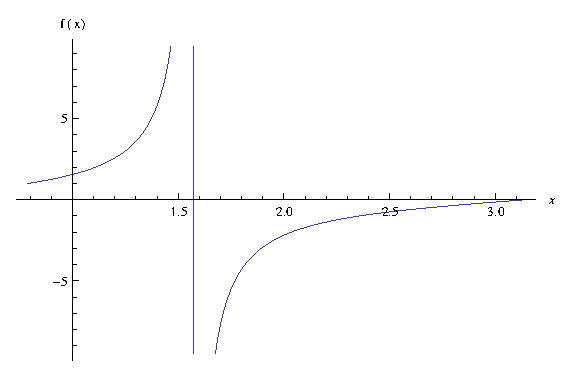
\includegraphics[scale=0.8]{graphs/tanx.eps}
        }
        \subfigure[\(f(x)=\arctan{x}\).]{
          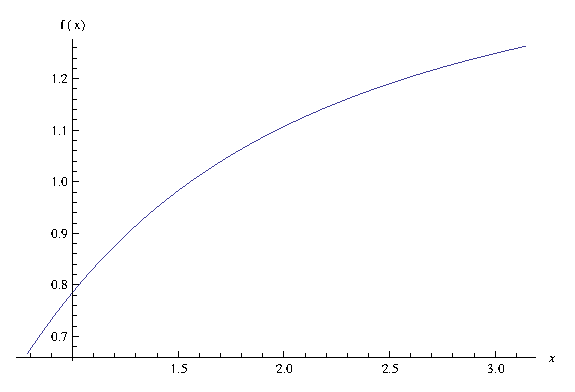
\includegraphics[scale=0.8]{graphs/arctanx.eps}
        }
    \end{center}
    \caption{\(\tan x\) compared with \(\arctan x\).}
  \end{figure}
  \end{sol}
\end{ex}
\begin{ex}
	\[ \int^0_{-\infty} \frac{x^2}{x^3-1} \]
	\begin{remark}
	  If $0 \to 1$, this would be a Type I integral.
	\end{remark}
	\begin{sol}
	  \begin{align*}
	  	\int^0_{-\infty} \frac{x^2}{x^3-1} &=\int^0_{-\infty} \frac{1}{3} \frac{\ud u}{u} \\
	  	&= \lim_{t \to \infty} \frac{1}{3}\ln{|x^3-1|\bigg|^0_t}
	  	= \lim_{t \to \infty} \frac{1}{3} \ln{|-1|}-\frac{1}{3}\ln{|t^3-1|} \\
	  	&= \lim_{t \to \infty} \frac{1}{3}ln{1}-\frac{1}{3}\ln{|t^3-1|} \\
	  	&= \lim_{t \to \infty} -\frac{1}{3}\ln{|t^3-1|}
	  \end{align*}
    The integral diverges.
  \end{sol}
\end{ex}
\begin{ex}
	\[ \int^0_{-\infty} e^x \ud u \]
	\begin{remark}
	  This is likely to converge, because of the $e^{-\infty}$.
	\end{remark}
	\begin{sol}
	\begin{align*}
		\int^0_{-\infty} e^x \ud u & =\lim_{t \to -\infty} e^x \bigg|^0_t \\
		&=\lim_{t \to -\infty} e^0-e^t
	\end{align*}
	The integral converges to $1$.
  \end{sol}
\end{ex}
\begin{ex}
	\[ \int^\infty_{-\infty} e^{-x} \cos x \ud x \]
	\begin{sol}
  First, break this into two parts.
	\begin{align*}
		\int^\infty_{-\infty} e^{-x} \cos x \ud x
		&=\int^0_{-\infty} e^{-x} \cos x \ud x+\int^\infty_0 e^{-x} \cos x \ud x \\
		\intertext{Then, treat it as an indefinite integral and evaluate using integration by parts:}
		\int e^{-x} \cos x \ud x&=\frac{e^{-x}\sin x - e^{-x} \cos x}{2}
		\intertext{Now, return to our original function.}
		\lim_{t \to \infty} e^{-x} \cos x \ud x
		&=\lim_{t \to \infty}
		  \frac{e^{-x}\sin x - e^{-x} \cos x}{2}\bigg|^0_t
		  -\frac{e^{-x}\sin x - e^{-x} \cos x}{2}\bigg|^t_0 \\
		&=\lim_{t \to \infty}
		  \left[\frac{e^{-0}\sin  - e^{-0} \cos 0}{2}
		  -\frac{e^{-t}\sin t - e^{-t} \cos t}{2}\right]
		  -\left[0+\frac{1}{2}\right] \\
	\end{align*}
	Because the left half of this diverges, the entire integral diverges.
\end{sol}
\end{ex}
\begin{ex}
  This is one of the classics:
	\[ \int^\infty_1 \frac{1}{x}\ud x \]
	\begin{sol}
	  Consider:
    \[ \int^\infty_1 \frac{1}{x^{1.000000001}}\ud x = x^{-0.000000001}\bigg|^\infty_1=0-\frac{1}{1^{0.000000001}}\]
    Therefore:
	  \begin{align*}
	  	\int^\infty_1 \frac{1}{x}\ud x
	  	&=\lim_{t \to \infty} \ln{|x|}\bigg|^t_1=\lim_{t \to \infty} \ln{|t|}-\ln{|1|} \\
	  	& =\lim_{t \to \infty} \ln{|t|}
	  \end{align*}
	  Diverges.
  \end{sol}
\end{ex}
\begin{ex}
  \[ \int^\infty_1 \frac{1}{x^2}\ud x =\lim_{t\to\infty}
    \frac{x^{-1}}{-1}\bigg|^t_1 \]
  This integral converges.
\end{ex}

\section{Test Review}

\begin{ex}
  \[\int \cot^2x \csc^4x \ud x \]
  \begin{sol}
    Set aside a $\csc^2x$.
    \begin{align*}
      \int \cot^2x \csc^4x \ud x
      =& \cot^2x \csc^2x \csc^2x \ud x
    \end{align*}
    Remembering our basic trig identity
    \[ \sin^2x + \cos^2x = 1\]
    we can divide through by $\sin^2x$ to get
    \[ 1+\cot^2x=\csc^2x \]
    and substitute that into our new integral
    \begin{align*}
      \int\cot^2x\csc^2x\csc^2x\ud x
      =& \int \cot^2x (1+\cot^2x)\csc^2x \ud x \\
      \intertext{Now we let $u=\cot x$ and $\ud u=\csc^2x \ud x$.}
      =&\int u^2(1+u^2)\ud u \\
      \intertext{which we can do.}
      =& \frac{u^3}{3}+\frac{u^5}{5}+C \\
      \intertext{Now replace our old $u$-substitutions}
      =& \frac{\cot^3x}{3}+\frac{\cot^5x}{5}+C
    \end{align*}
  \end{sol}
\end{ex}
\begin{ex}
  \[ \int \tan x \sec^4x \ud x \]
  \begin{sol}
    Set aside a $\sec^2x$
    \begin{align*}
      \int \tan x\sec^4x \ud x
      = \int \tan x \sec^2 x \sec^2 x \ud x
    \end{align*}
    Remembering our basic trig identity
    \[ \sin^2x + \cos^2x = 1\]
    we can divide through by $\cos^2x$ to get
    \[ \tan^2x+1=\sec^2x \]
    and substitute that into our new integral
    \begin{align*}
      \int \tan x \sec^2 x \sec^2 x \ud x
      =& \int \tan x (\tan^2x-1) \sec^2x \ud x \\
    \end{align*}
    Now let $u=\tan x$ and $\ud u = \sec^2x \ud x$
    \begin{align*}
      \int \tan x (\tan^2x-1) \sec^2x \ud x
      =& \int u (u^2-1) \ud u \\
      =& \frac{u^3}{3}-\frac{u^2}{2}+C \\
      =& \frac{\tan^3x}{3}-\frac{\tan^2x}{2} +C
    \end{align*}
  \end{sol}
\end{ex}
\begin{ex}
  \[ \int x^2 e^x \ud x \]
  \begin{sol}
    \begin{align*}
      \int x^2 e^x\ud x
      =& x^2 e^x-2\int x e^x \ud x \\
      =& x^2 e^x -2 \left( x e^x - \int e^x \ud x \right) \\
      =& x^2 e^x -2 x e^x +2x +C
    \end{align*}
  \end{sol}
\end{ex}
\begin{ex}
  \[ \int^4_2 \frac{1}{x-4}\ud x \]
  \begin{sol}
    \begin{align*}
      \int^4_2 \frac{1}{x-4}\ud x
      =& x\ln{|x-4|}\bigg|^t_2 \\
      =& \ln{|t-4|}-\ln{|-2|}
    \end{align*}
    Now we go back to the original integral
    \[
      \int^4_2 \frac{1}{x-4}\ud x
      = \lim_{t \to 4^-}\ln{|t-4|}-\ln 2
      \]
      Remembering the graph of \(\ln{|x|}\)
      \begin{figure}[H]
        \begin{center}
          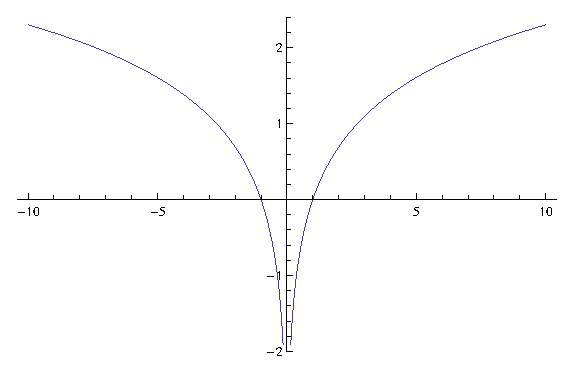
\includegraphics[scale=1]{graphs/logabsx.eps}
        \end{center}
        \caption{A plot of \(f(x)=\ln{|x|}\)}
      \end{figure}
      we can conclude that the integral diverges toward $-\infty$.
  \end{sol}
\end{ex}
\begin{ex}
  \[ \int^6_5 \frac{1}{(x-5)^{1/2}}\ud x \]
  \begin{sol}
    \begin{align*}
      \int^6_t \frac{1}{(x-5)^{1/2}}\ud x
      =& 2 \sqrt{x-5}\bigg|^6_t \\
      =& 2 \sqrt{6-5}-2\sqrt{t-5}
    \end{align*}
    \begin{align*}
      \int^6_5 \frac{1}{(x-5)^{1/2}}\ud x
      =& \lim_{t \to 5^+} 2\sqrt{6-5}-\underbrace{2\sqrt{t-5}}_{0} \\
      =& \lim_{t \to 5^+} 2\sqrt{6-5}\\
      =& 2
    \end{align*}
  \end{sol}
\end{ex}
\begin{ex}
  \[ \int^\infty_{\frac{8\sqrt 3}{3}}\frac{1}{x^2+64}\ud x \]
  \begin{sol}
    \begin{align*}
      \int \frac{1}{x^2-64}\ud x
      =& \int \frac{1}{64(\frac{x^2}{64}+1)} \\
      =&\frac{1}{8}\arctan{\frac{x}{8}} + C
    \end{align*}
    \begin{align*}
      \int^t_{\frac{8\sqrt 3}{3}}\frac{1}{x^2+64}\ud x
      =&\frac{1}{8}\arctan{\frac{x}{8}}\bigg|^t_{\frac{8\sqrt 3}{3}} \\
    \end{align*}
    \begin{align*}
      \int^\infty_{\frac{8\sqrt 3}{3}}\frac{1}{x^2+64}\ud x
      =& \lim_{t \to \infty} \frac{1}{8}\arctan{\frac{t}{8}}-\frac{1}{8}\arctan{\frac{\sqrt 3}{3}} \\
      =& \frac{1}{8}\left(\frac{\pi}{2}-\frac{\pi}{6}\right) \\
      =& \frac{\pi}{24}
    \end{align*}
  \end{sol}
\end{ex}
\begin{ex}
  \[\int x^3 \cos{3x} \ud x\]
  \begin{sol}
    We use integration by parts.
    \begin{align*}
      \int x^3 \cos{3x} \ud x
      =& \frac{1}{3}x^3\sin{3x}-\int x^2 \sin{3x}\ud x \\
      =& \frac{1}{3}x^3\sin{3x}-\left[
        \frac{-1}{3}x^2\cos{3x}+\frac{2}{3}\int x \cos{3x} \ud x
        \right] \\
        =& \frac{1}{3}x^3\sin{3x}+\frac{1}{3}x^2\cos{3x}-\frac{2}{3}\left[\frac{1}{3}x\sin{3x}-\frac{1}{3}\int \sin{3x}\ud x\right] \\
        =&\frac{1}{3}x^3\sin{3x}+\frac{1}{3}x^2\cos{3x}-\frac{2}{9}x\sin{3x}-\frac{2}{27}\cos{3x}+C
    \end{align*}
  \end{sol} \end{ex}

% \begin{homework}
%   Chapter 8 test on Friday, March 16, 2012.
% \end{homework}



\chapter{Sequences}
\label{ch:sequences}

%\begin{quote}
%  \emph{``Sequences are fundamental to the study of infinite series and many
%  applications of mathematics.''}
%
%\hfill\cite[p.~532]{thomas}
%\end{quote}
A \textbf{sequence}\index{sequence} is an ordered list of numbers. They are mostly important because of their application to \textbf{series},
detailed in Chapter \ref{ch:series}.
\section{Representing a Sequence}
\begin{defn}
  A \textbf{sequence} is a list of numbers
  \[ a_1, a_2, a_3, \ldots, a_n, \ldots\]
  in a given order. This order is important: The sequence \(2, 4, 6, 8, \ldots\) is not the same as the sequence \(4, 2, 8, 6, \ldots\).
\end{defn}
When we write sequences like \(\{a_n\}\), we are talking about the entire
sequence. A sequence like this is described as ``starting at'' a certain \emph{index},
usually \(n=1\). In the context of the series we'll be using, they are normally infinite
in length.

We can also write sequences using rules that describe their
terms, as follows:

\begin{ex}
\[ a_n = \frac{n!}{2n!+1} \]
  We can write out a few terms of the sequence
  \[
    \left\{
      \frac{1}{3},\frac{2}{5},\frac{6}{13},\frac{24}{49},\frac{120}{241},
    \ldots \right\}
  \]
  and then plot them %(shown in figure \ref{fig:firstsequence})
  to get a feel that the
  sequence is getting closer and closer to a certain number: \[ \frac{1}{2}.\] We would
  thus describe this sequence as \emph{converging to} the number \( \frac{1}{2} \)
% BROKEN FIGURE
%  \begin{figure}[h]
%    \begin{center}
%      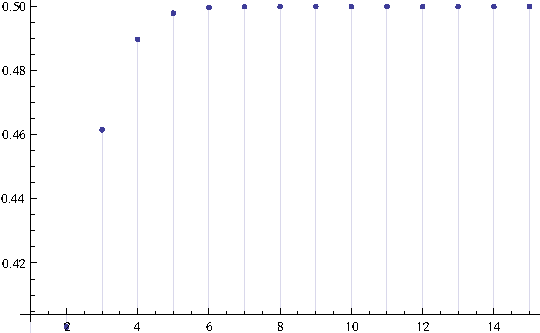
\includegraphics{graphs/nf2nfp1.pdf}
%    \end{center}
%    \label{fig:firstsequence}
%    \caption{A plot of \( a_n = \frac{n!}{2n!+1} \)}
%  \end{figure}
\end{ex}
\begin{defn}\index{converging sequence}
  The sequence \(\{ a_n \}\) \textbf{converges} to the number \(L\) if for every
  positive number \(\varepsilon\) there corresponds an integer \(N\) such that
  for all \(n\)
  \[ n > N \to |a_n - L| < \varepsilon \]
  If \(\{a_n\}\) converges to \(L\), we write \(\lim_{n \to \infty} a_n = L\),
  and call \(L\) the \emph{limit} of the sequence.
\end{defn}
  To really understand this, try thinking of it this way: pick a number $\varepsilon$. It can be very large
  \[ \varepsilon=1000\]
  or really small
  \[ \varepsilon=0.0001\]
  but no matter which one we pick, we can find an index $N$ on the sequence such that for every index past it, we
  are always within $\varepsilon$ of the limit $L$ for the sequence.
  Note that we don't have to know what this number $L$ is, nor what $\varepsilon$ is for that matter, just that
  these numbers exist to state that a sequence is \emph{converging}.
\begin{ex}
  Let us examine the following imaginary sequence:
  \begin{figure}[H]
    \begin{center}
      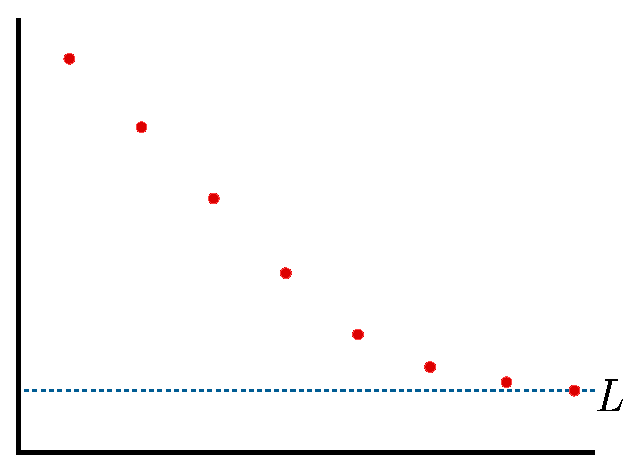
\includegraphics[scale=0.5]{continuous/sequence/conv1}
    \end{center}
    \label{fig:conv1}
  \end{figure}
  Note that for a large $\varepsilon$, our corresponding $N$ occurs very early in the sequence:
  \begin{figure}[H]
    \begin{center}
      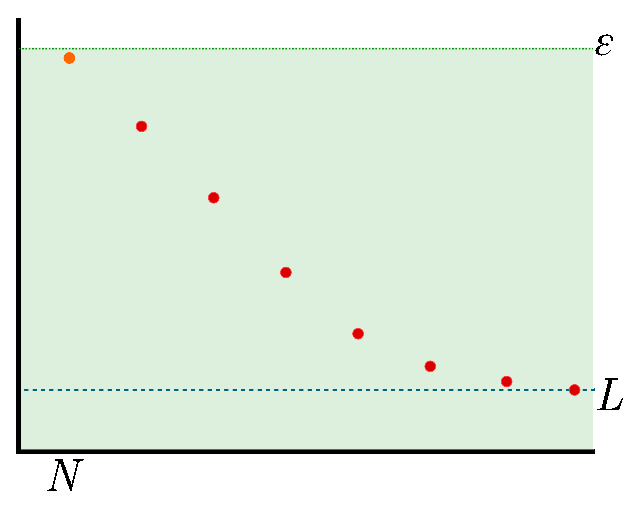
\includegraphics[scale=0.5]{continuous/sequence/conv2}
    \end{center}
    \label{fig:conv2}
  \end{figure}
  However, if we shrink our $\varepsilon$, the number $N$ needed such that every element in the sequence after it
  is within $\varepsilon$ of $L$ gets larger. The real key, however, is that it \emph{always exists}.
  \begin{figure}[H]
    \begin{center}
      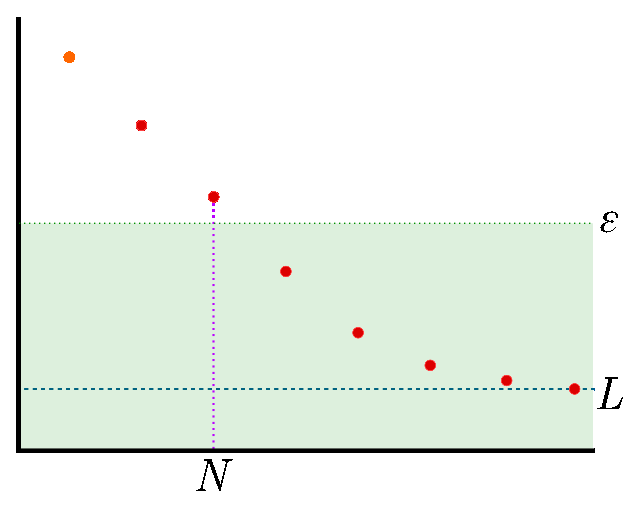
\includegraphics[scale=0.5]{continuous/sequence/conv3}
    \end{center}
    \label{fig:conv3}
  \end{figure}
\end{ex}
\begin{defn}\index{diverging sequence}
  The sequence \(\{ a_n \}\) \textbf{diverges} if the sequence does not converge
  to any number \(L\).

  That is, this number $L$ does not exist.
\end{defn}

\subsection{Bounded Sequences}
\begin{defn}\index{lower bound}
  If there exists a number $m$ such that $m \leq a_n$ for every $n$ we say the sequence is \textbf{bounded below}.
  The number $m$ is called a \textbf{lower bound} for the sequence.
  \begin{figure}[h]
    \begin{center}
      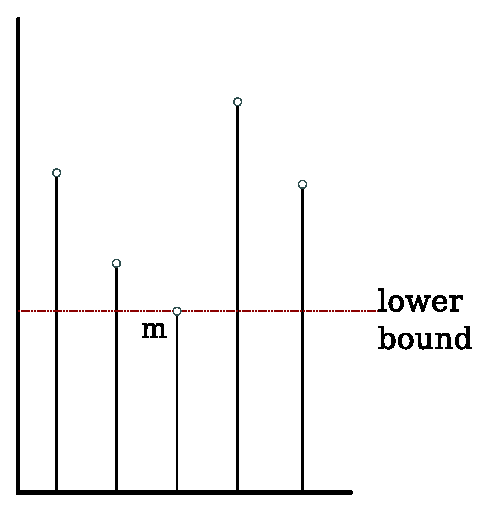
\includegraphics[scale=0.5]{continuous/sequence/lwrbnd}
    \end{center}
  \end{figure}
\end{defn}
\begin{defn}\index{upper bound}
  If there exists a number $M$ such that $a_n \leq M$ for every $n$ we say that the sequence is \textbf{bounded above}.
  The number $M$ is called an \textbf{upper bound} for the sequence.
  \begin{figure}[h]
    \begin{center}
      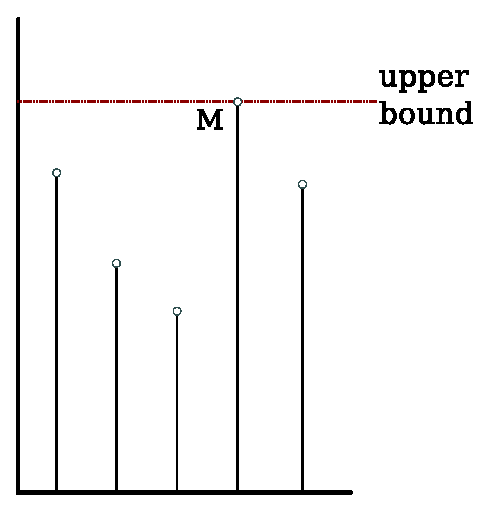
\includegraphics[scale=0.5]{continuous/sequence/uprbnd}
    \end{center}
  \end{figure}
\end{defn}
\begin{defn}\index{bounded}
  If the sequence is both bounded below and bounded above we call the sequence \textbf{bounded}.
\end{defn}
\subsection{Nondecreasing and Nonincreasing Sequences}\label{nondecreasing}
\begin{defn}\index{nondecreasing}
  Given a sequence \(\{a_n\}\), we call the sequence \textbf{nondecreasing} if
  \[\forall n (a_n \geq a_{n-1}).\]
  This means that across the entire sequence, a given element in the sequence is either greater than or equal to the preceeding element.
  A nondecreasing sequence is different from a strictly \emph{increasing} sequence in that it allows for two elements to be equal.
  \begin{figure}[H]
    \begin{center}
      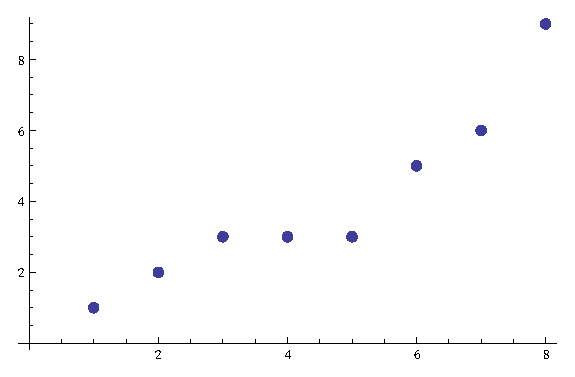
\includegraphics[scale=0.5]{continuous/sequence/nondecreasing}
    \end{center}
    \caption{This sequence is not \emph{increasing} everywhere, although it is \emph{nondecreasing}.}
  \end{figure}
\end{defn}
\begin{defn}
  Given a sequence \(\{a_n\}\), we call the sequence \textbf{nonincreasing} if
  \[\forall n (a_n \leq a_{n-1}).\]
\end{defn}
\begin{defn}
  If \(\{a_n\}\) is either nondecreasing or nonincreasing we call it \textbf{monotonic}.
  \begin{figure}[H]
    \begin{center}
      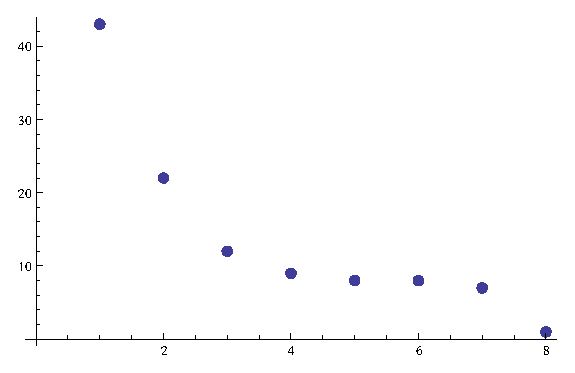
\includegraphics[scale=0.5]{continuous/sequence/nonincreasing}
    \end{center}
    \caption{An example of a nonincreasing sequence.}
  \end{figure}
\end{defn}

\begin{ex}\label{ex:bigsequence}
  \[ a_n=\frac{n+1}{2n-1} \]
    Let's take a more detailed look at an example of a sequence.

    To get a feel for the behavior of the sequence, let's find a few of its
    values:
    \[ \frac{n+2}{2n-1} =
      \left\{3,\frac{4}{3},1,\frac{6}{7},\frac{7}{9},\frac{8}{11}, \cdots \right\} \]


    We could take the derivative of the similar function
    \[ f(x)=\frac{x+2}{2x-1} \]
    to try to figure out what is happening. Since we can assume \(n \geq 1\) for
    our sequence, for \(x \geq 1\) the derivative of \(f(x)\) should also be
    somewhat representative of \(a_n\).
    \begin{align*}
      f'(x)&= \frac{(2 x-1) \left(\frac{\ud}{\ud x}(x+2)\right)-(x+2)
      \left(\frac{\ud}{\ud x}(2 x-1)\right)}{(2 x-1)^2}
      \\
      &=\frac{2 x-2 (x+2)-1}{(2 x-1)^2} \\
      &=-\frac{5}{1-4 x+4 x^2}
    \end{align*}
    \begin{table}[h]
      \centering
      \boxed{
        \begin{tabular}{>\(r<\)|>\(c<\)|>\(c<\)|>\(c<\)}
          x & 0 & 0.5 & 1 \\ \hline
          f'(x) & - & \text{undefined} & -
        \end{tabular}
      }
      \caption{A sign diagram for \(f'(x)\).}
      \label{tab:n51m2xs}
    \end{table}
    \begin{figure}[h]
      \begin{center}
        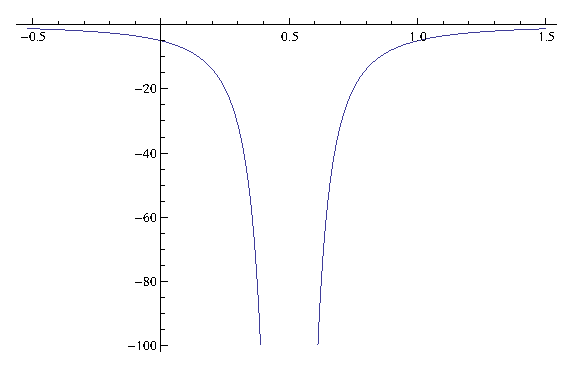
\includegraphics{graphs/n51m2xs}
      \end{center}
      \caption{A plot of \(f'(x)\).}
      \label{fig:n51m2xs}
    \end{figure}
    Based on Table \ref{tab:n51m2xs}, we can conclude that the sequence is
    nonincreasing. We can therefore describe this sequence as \emph{monotonic}.

    Furthermore, note the end-behavior of this derivative:
    \[ \lim_{x \to \infty} f'(x) = 0 \]
    This implies that, eventually, the rate of change evens off to an indefinitely small number.
    Presumably, this would mean that \(f(x)\) has a horizontal asymptote.
    Based on this information, it seems reasonable to conclude that the sequence \(a_n\) is convering upon a number.
    We do not, however, know to what number it converges.

    To find that, we will need to take the following limit:
    \[ \lim_{n\to\infty} a_n \]
    How do we evaluate limits for sequences? As it turns out, we usually treat
    them exactly the same as limits as functions.
    \begin{theorem}\label{inftyanlimit}\index{limits of sequences}
      Suppose that \(f(x)\) is a function defined for all \( x \geq n_0\) and
      that \( \{a_n\} \) is a sequence of real numbers such that \(a_n = f(n)\)
      for \(n \geq n_0\). Then
      \[ \lim_{x \to \infty} f(x) = L \to \lim_{n \to \infty} a_n = L\text{.} \]
      \begin{proof}
        Suppose that \( \lim_{x \to \infty} f(x) = L \). Then for each positive
        number \( \varepsilon \) there is a number \( M \) such that for all
        \(x\),
        \[ x > M \implies \big| f(x) - L \big| < \varepsilon \]
        Let \(N\) be an integer greater than \(M\) and greater than or equal to
        \(n_0\). Then
        \[ n > N \implies a_n = f(n)\]
        and
        \[\big|a_n -L \big| = \big|f(n) - L\big| < \varepsilon\text{.} \qedhere\]
        \cite[p. 537]{thomas}%Thomas' Calculus, p. 537
      \end{proof}
    \end{theorem}
    This allows us to use \emph{l'Hospital's Rule} to find the limits of some
    sequences. We can state that
    \[\lim_{n\to\infty} a_n =\lim_{n\to\infty}f(x)\]
    assuming
    \[f(x)=\frac{n+1}{2n-1}\text{.}\]
    And thus evaluate the following limit:
    \begin{align*}
      \lim_{n\to\infty} \frac{n+1}{2n-1}
      &\=H \lim_{n\to\infty} \dfrac{\frac{\ud}{\ud x}(n+1)}{\frac{\ud}{\ud x}2n-1} \\
      &\=H \lim_{n\to\infty} \frac{1}{2} \\
      &= \frac{1}{2}
    \end{align*}
    This shows us that the sequence $a_n$ also converges to \(\frac{1}{2}\).
    \begin{figure}[H]
      \begin{center}
        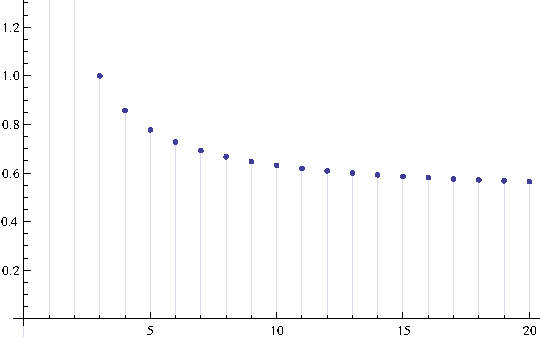
\includegraphics{graphs/np22nm1.pdf}
      \end{center}
      \caption{A graph of the sequence $ a_n=\frac{n+1}{2n-1} $.}
    \end{figure}
\end{ex}
\begin{ex}
  Demonstrate that $\{n!\}$ is nondecreasing.
  \begin{sol}
    First let us look at the definition for a factorial.
    \begin{equation}\label{eq:factorial}\index{factorial}
      n! =
      \begin{cases}
        1 & \text{if } n = 0, \\
        n(n-1)! & \text{if } n > 0
      \end{cases}
    \end{equation}
    \begin{proof}
      Remember our definition for a nondecreasing sequence from \ref{nondecreasing}:
      \[\forall n (a_n \geq a_{n-1})\text{.}\]
      Let us assume that this holds true for our sequence $\{n!\}$ when $n>1$.
      \begin{align*}
        n!&\geq(n-1)!& n&>1 \\
        \intertext{Divide each side by $(n-1)!$}
        \frac{n!}{(n-1)!}&\geq \frac{(n-1)!}{(n-1)!} &n&>1 \\
        \frac{n!}{(n-1)!}&\geq 1 &n&>1 \\
        \intertext{Now, remembering our definition for the factorial,}
        \frac{n(n-1)!}{(n-1)!}&\geq 1 &n&>1 \\
        n&\geq1 &n&>1\qedhere
      \end{align*}
    \end{proof}
    % \begin{proof}
    %   \begin{align*}
    %     \underbrace{n!}_{n(n-1)} > (n-1)!
    %     n(n-1)! &> (n-1)! \\
    %     n(n-1)! - (n-1)! &> 0 \\
    %     (n-1)! [n-1] &> 0 \qedhere
    %   \end{align*}
    % \end{proof}
  \end{sol}
\end{ex}
\begin{ex}
  Show that the sequence \[ \{a_n\} = \left\{ \frac{n+2}{2n-1} \right\}^{\infty}_{n=1} \] is nonincreasing.
  \begin{sol}
    This example is very similar to Example \ref{ex:bigsequence}, with only a
    change of constant in the numerator. We will demonstrate this sequence's
    behavior using a different method than before, however.

    Another way we can demonstrate that a sequence is decreasing is by using
    the definition of a \emph{decreasing sequence}: \(\forall n ( a_n <
    a_{n-1})\). We simply substitute in \(n\) and \(n-1\) on the
    respective sides of the inequality.
    \begin{proof}
      \begin{align*}
        \forall n (a_n &< a_{n-1}) &n&>1 \\
        \frac{n+2}{2n-1} &< \frac{(n-1)+2}{2(n-1)-1} &n&>1 \\
        \frac{n+2}{2n-1} &< \frac{n+1}{2n-3} &n&>1 \\
        \left(\frac{2n-3}{2n-3}\right) \left( \frac{n+2}{2n-1} \right)
        &< \left(\frac{n+1}{2n-3}\right) \left(\frac{2n-1}{2n-1}\right)
        &n&>1\\
        \frac{2n^2-3n+4n-6}{4n^2-6n-2n+3} &< \frac{2n^2+2n-n-1}{4n^2-6n-2n-3} &n&>1\\
        \frac{2n^2+n-6}{4n^2-8n+3}&<\frac{2n^2+n-1}{4n^2-8n-4} &n&>1 \\
        2n^2+n-6 &< 2n^2+n-1 &n&>1 \\
        -6 &< -1 &n&>1 \qedhere
      \end{align*}
    \end{proof}
  \end{sol}
\end{ex}
% \begin{ex}
%   Is
%   \[ \left\{\frac{n}{n+1} \right\} \]
%   monotonic?
%   \begin{sol}
%       \begin{align*}
%         \lim_{n\to\infty} \frac{n}{n+1}=1
%       \end{align*}
%       \begin{align*}
%         f(x)&=\frac{x}{x+1} \\
%         f'(x)&=\frac{(x+1)1-x(1)}{(x+1)^2} \\
%         f'(x)&=\frac{1}{(x+1)^2}
%       \end{align*}
%   \end{sol}
% \end{ex}
\begin{ex}
  Show that
  \[ \left\{ \frac{n}{n+1} \right\} \]
  is monotonic increasing.
  \begin{sol}
    \begin{proof}
      \[ \forall n > 1 \left(  a_n > a_{n-1}  \right) \]
      \begin{align*}
        a_n &> a_{n-1}\\
        \frac{n}{n+1} &> \frac{n-1}{n-1+1} \\
        \frac{n}{n} \frac{n}{n+1} &> \frac{n-1}{n}\frac{n+1}{n+1} \\
        n^2 &> (n-1)(n+1)\\
        n^2 &> n^2-1 \\
        0 &> -1 \qedhere
      \end{align*}
    \end{proof}
  \end{sol}
\end{ex}
\begin{ex}
  Does
  \[ a_n = \frac{n+1}{2^n} \]
  converge or diverge?
  \begin{sol}
    Remembering that we can rewrite \(2^n\) as
          \( e^{n \cdot \ln{2}} \)
    \begin{align*}
      \lim_{n \to \infty} \frac{n+1}{2^n}
      &= \lim_{n \to \infty} \frac{n+1}{e^{n\cdot \ln{2}}} \\
      &\=H \lim_{n \to \infty} \frac{1}{\ln2 \cdot e^{n\ln2}}\\
      &= \lim_{n \to \infty} \frac{1}{\ln2 \cdot 2^n}
      \intertext{Using the constant multiple rule for limits of sequences, we
      can pull out the \( \ln 2 \). }
      &= \frac{1}{\ln 2}\cdot \left(\lim_{n \to \infty}
      \frac{1}{2^n}\right)
    \end{align*}
    \(\{\frac{1}{2^n}\}\) is converging very quickly toward 0,
    so \(a_n\) as well must converge to \(0\).
    \begin{figure}[h]
      \begin{center}
        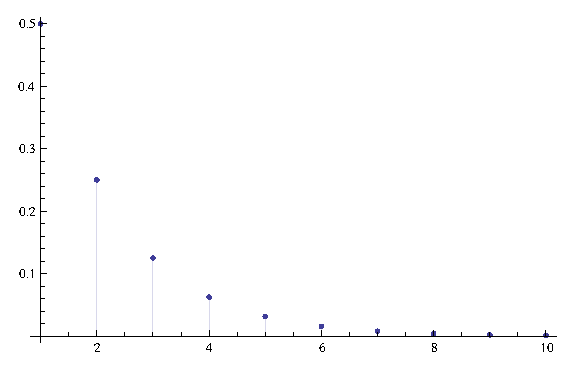
\includegraphics{graphs/oneovertwoton}
      \end{center}
      \caption{A plot of \(\{\frac{1}{2^n}\}\).}
      \label{fig:oneovertwoton}
    \end{figure}
  \end{sol}
\end{ex}
\begin{ex}
  Does
  \[ \left\{ \frac{1}{n!} \right\} \]
  converge or diverge?
  \begin{sol}
      \begin{align*}
        \lim_{n \to \infty} \frac{1}{n!} = 0
      \end{align*}
  \end{sol}
  Alternatively, we could demonstrate that the sequence is bounded and monotonic.
\end{ex}
\begin{ex}
  Does
  \[ a_n = \frac{2^n}{n!} \]
  converge or diverge?
  \begin{sol}
    We can show this, intuitively, as follows:
    \begin{align*}
      a_n = \left\{
        \frac{2\times2\times2\times2\times2\times\ldots}{1+2+3+4+5+6+\ldots} \right\}
    \end{align*}
    But the actual proof requires the \emph{sandwich theorem for
    sequences}\cite[p.~536]{thomas}:
    \begin{theorem}[The Sandwich Theorem for Sequences]\index{The Sandwich
      Theorem for Sequences}\label{th:sandwichsequence}
      Let $\{a_n\}$, $\{b_n\}$, and $\{c_n\}$ be sequences of real numbers. If
      $a_n \leq b_n \leq c_n $ holds for all $n$ beyond some index $N$, and if
      $\lim_{n\to\infty} a_n = \lim_{n\to\infty} c_n = L$, then
      $\lim_{n\to\infty} b_n = L$ also.
    \end{theorem}
      A proof of this theorem is found in \ref{proof:sandwichsequence}.
      By Theorem \ref{th:sandwichsequence}, \[\lim_{n \to \infty} a_n =
      \lim_{n\to\infty}\frac{2^n}{n!}=0.\]
  \end{sol}
\end{ex}
\begin{ex}
  \[ a_n = \frac{(-1)^n}{n!} \]
  \begin{sol}
    Consider
    \begin{align*}
      b_n = \left| \frac{(-1)^n}{n!} \right| = \frac{1}{n!} = 0
    \end{align*}
    Intuitively, we can also state that $a_n$ should converge.
    Using Theorem \ref{th:sandwichsequence}, we can determine that this sequence converges.
    % Review \emph{bounded and monotonic} for sequences, txtbg pg 536.
    % That's in Thomas' calculus. -[Nathan]
  \end{sol}
\end{ex}
\begin{ex}
  \[ a_n = \frac{1}{n-0.\bar{9}} \]
  \begin{sol}
    A sequence can be unbounded, and still converge.

    $0.\bar{9}$ is very close to $1$, close enough that we can treat it as $1$ as $n\to\infty$.
    Doing so, it becomes clear that this sequence converges, as $\frac{1}{n-1}$ converges.
    Consider, however, the very first term, where $n=1$.
    This term is \emph{gigantic}, essentially \(\infty\).
    The sequence is not bounded, yet it still manages to converge.
    This sequence converges to \(0\).
  \end{sol}
\end{ex}
\begin{ex}
  Does the following sequence converge?
  \[ a_n = \left( \frac{n+8}{9n} \right) \left( 1-\frac{8}{n} \right) \]
  Find the limit if the sequence is convergent.
  \begin{sol}
    Remembering that a limit of products is a product of limits,
    \begin{align*}
      \lim_{n \to \infty} \left( \frac{n+8}{9n} \right) \left( 1-\frac{8}{n} \right)
      &= \lim_{n \to \infty} \left( \frac{n+8}{9n} \right) \cdot
      \lim_{n \to \infty} \left( 1-\frac{8}{n} \right)\\
      &= \frac{1}{9}
    \end{align*}
    The sequence converges to \(\frac{1}{9} \).
  \end{sol}
\end{ex}
\begin{ex}
  Show that the sequence \[a_n = \frac{2}{n^2} \] is monotonic and bounded.
  \begin{sol}
    Treat the sequence as a function $f(x)$ and take the derivative.
    \[ f(x) = \frac{2}{x^2} \]
    \[ f'(x) = -4 x^{-3} \]
    $f'(x)$ is negative on the interval $[1, \infty)$, so $f(x)$ is decreasing
      on the interval $[1, \infty)$. Since the sequence goes from $1$ to
        $\infty$ and is always decreasing, its upper bound must be at $n=1$.
        $a_1=2$, the upper bound for the sequence. To find the lower bound, we
        take the limit as $n \to \infty$:
        \[ \lim_{n \to \infty} a_n = \lim_{n \to \infty} \frac{2}{n^2} = 0 \]
        Which shows us that $0$ is the lower bound of the sequence.

        Thus, we can conclude that the sequence is monotonic and bounded, and therefore converges.
  \end{sol}
\end{ex}
\begin{ex}
  Find a formula for the nth term of the sequence where \(a_n\) is calculated
  directly from \(n\).
  \[ \frac{1}{1}, \frac{4}{2}, \frac{7}{6}, \frac{10}{24}, \frac{13}{120} \cdots \]
  \begin{sol}
    We basically have to just take close guesses and see if we can make a sequence that follows this.

    Doing so, we will find that the answer is
    \[ a_n = \frac{3n-2}{n!}.\]
  \end{sol}
\end{ex}

% \begin{homework}
%     Wolfram Mathematica assingment and MyMathLab homework due Friday, March 23, 2012.
% \end{homework}
% \begin{homework}
%   Read Section 10.2
%
%   pg. 551 ALL 27-34, 35, 36, 37, 38, 41, 43, 49, 50, 51, 55, 56, 57, 58, 59, 61
% \end{homework}
%

\chapter{Infinite Series}
\label{ch:series}

An infinite series is the sum of an infinite sequence of numbers
\[ a_1 + a_2 + a_3 + \cdots + a_n + \cdots \]
Given a sequence $\{a_n\}$, the number $a_n$ is the \textbf{$n$th term} of the
series. The sequence $\{s_n\}$ is the \textbf{sequence of partial sums} of the
series, defined by
\begin{align*}
  s_1 &= a_1 \\
  s_2 &= a_1 + a_2 \\
  & \vdots \\
  s_n &= a_1 + a_2 + \cdots + a_n = \sum^\infty_{k=1} a_k \\
  & \vdots
\end{align*}
The number $s_n$ represents the \textbf{$n$th partial sum} of the infinite
series.

The partial sum \(s_n\) of a series can also be given by
  \[ s_n = s_{n-1} + a_n .\]

If the sequence of partial sums converges to a limit $L$, we say that
the series \textbf{converges} and that its \textbf{sum} is $L$. In this case, we
also write
\[ a_1 + a_2 + a_3 + \cdots + a_n + \cdots = \sum_{n=1}^\infty a_n = L \]
If the sequence of partial sums of the series does not converge, then we say
that the series \textbf{diverges}.
\cite[p.~544]{thomas}

Given a series, we will usually want to know whether it converges or diverges,
and if it converges, then to what number?

For converging series, there are some rules that can aid us:
\begin{theorem}\label{th:combiningseries}
  If $\sum a_n = A$ and $\sum b_n = B$ are convergent series, then
  \begin{table}[H]
    \centering
    \begin{tabular}{ll>$r<$}
    1. & Sum Rule & \sum (a_n+b_n) = \sum a_n + \sum b_n = A +B \\
    2. & Difference Rule & \sum (a_n-b_n) = \sum a_n - \sum b_n = A -B \\
    3.& Constant Multiple Rule & \sum ka_n = k\sum a_n = kA \text{ for any
    $k$}
    \end{tabular}
  \end{table}
\end{theorem}

% \begin{remark}
%   When discussing a series,
%   \[
%     \sum{i=1}^\infty f(x) \text{ is better written }\sum{i=1}^\infty a_n
%     \text{.}
%   \]
% \end{remark}

\section{Limit Test}\index{series limit test}

When presented with a series, such as
\[ \sum^\infty_{n=1} \frac{n!}{2n!+1}, \]
if we wish to know whether it converges or diverges, we should generally first
confirm that the series does not diverge before trying to determine its
convergence.

For a series like this, it is better to think of it as a sum of numbers in a
sequence, $\{a_n\}$, than as a sum operator operating on a function. In this
case, $\{a_n\}$ would equal
\[ \frac{n!}{2n!+1} \]

Now think about it--if this $\{a_n\}$ is converging to any number other than
$0$, then as our $n$ goes toward $\infty$, we will always have numbers to add.
The sequence will continue growing. That is, the sequence will diverge.

So we should take the following limit:
\[ \lim_{n \to \infty} \frac{n!}{2n!+1} \]
How do we calculate the limit of a sequence involving $n!$? Our limit rules tell
us nothing about evaluating factorials. We can, however, use a creative little trick
common in evaluating limits of polynomials: divide each term in both the
numerator and denominator by the term of the highest power.
\begin{align*}
  \lim_{n \to \infty} \frac{n!}{2n!+1} &=
  \frac{\frac{n!}{n!}}{\frac{2 \cdot n!}{n!}+\frac{1}{n!}} \\
  &= \frac{1}{2 + \frac{1}{n!}} \\
  \intertext{Now, think about where the term $\frac{1}{n!}$ is heading as $n
  \to \infty$. The denominator is getting huge, and very quickly, as if there
  were a high degree power of $x$ in the denominator of a limit. In that case,
  $1/x^k$ would become meaningless--it would essentially disappear, so $1/n!$
  must also go to $0$.}
  &= \frac{1}{2+0} \\
  \lim_{n \to \infty} a_n &=\frac{1}{2}
\end{align*}
So the limit of $\{a_n\}$ as $n$ approached $\infty$ is not zero. Thus, the
\emph{$n$th term} of the series, no matter how large $n$ becomes, will never be
zero. The series is always adding more numbers, and that means it is
\textbf{diverging}.

It is worth noting that if, indeed, the \(\lim_{n\to \infty}\) of \( \{a_n\} \) did equal $0$, this would
tell us nothing about the convergence or divergence of the series.

\begin{theorem}\label{th:nthtermdiv}
  The series $\sum^\infty_{n=1} a_n$ diverges if \(\lim_{n\to \infty} a_n \neq 0
  \).
  \begin{proof}
    We prove this by contrapositive, described in Section
    \ref{app:def:contrapositive}. The statement we are trying to prove is:
    \begin{quote}
      If \(\lim_{n\to \infty} a_n \neq 0 \) then the series diverges.
    \end{quote}
    We could write this as $P \to Q$ where $P$ represents ``The limit of $a_n$
    as $n \to \infty$ is nonzero'' and $Q$ represents ``the series diverges.''
    Thus, the contrapositive of this proposition would be $\neg Q \to \neg P$.
    If we can prove the contrapositive, then the original statement must be
    true.
    We would $\neg Q \to \neg P$ as:
    \begin{quote}
      ``If a series is convergent, then \( \lim_{n \to \infty} a_n = 0\).''
    \end{quote}
    Now, let $L$ represent the series' sum.
    \begin{align*}
      s_n &= s_{n-1} + a_n \\
      \lim_{n \to \infty} s_n &= \lim_{n \to \infty} s_{n-1} + a_n \\
      L&=L + \lim_{n\to \infty} a_n \\
      \lim_{n\to \infty} a_n &= 0\qedhere
    \end{align*}
  \end{proof}
\end{theorem}

\begin{ex}
  Does the series
  \[ \sum^\infty_{n=1} \frac{6n}{6n+1} \]
  diverge or converge?
  \begin{sol}
    Take \( \lim_{n\to\infty} \frac{6n}{6n+1} \).
    \begin{align*}
      \lim_{n\to\infty} \frac{6n}{6n+1}
      &\=H \lim_{n\to\infty} \frac{6}{6} \neq 0
    \end{align*}
    By Theorem \ref{th:nthtermdiv}, the series diverges.
  \end{sol}
\end{ex}

\section{Harmonic Series}

\begin{ex}
  The series
  \[ \sum_{n=1}^{\infty} \frac{1}{n} \]
  is called the \textbf{harmonic series}. How does this series behave?
  \begin{remark}
    Just because
    \[ \lim_{n \to \infty} \frac{1}{n}\]
    is zero does not imply anything about convergence or divergence.
  \end{remark}

  We can try finding some of its partial sums:
  \begin{align*}
    s_1 & = 1 \\
    s_2 & = 1 + \frac{1}{2} \\
    s_3 & = 1 + \frac{1}{2} + \frac{1}{3} \\
    s_4 & = 1 + \frac{1}{2} + \frac{1}{3} + \frac{1}{4} \\
    &\vdots \\
    s_n & = 1 + \frac{1}{2} + \frac{1}{3} + \frac{1}{4} + \cdots + a_n
  \end{align*}
  Notice that as we continue to add terms, we could group them in the following
  way:
  \begin{align*}
    s_n &= 1 + \frac{1}{2} + \bigg( \frac{1}{3} + \frac{1}{4} \bigg)
    + \bigg( \frac{1}{5} + \frac{1}{6} + \frac{1}{7} + \frac{1}{8} \bigg)
    + \bigg( \frac{1}{9} + \frac{1}{10} + \cdots + \frac{1}{16} \bigg)
    + \cdots\\
    &= 1 + \frac{1}{2} + \bigg( \frac{7}{12} \bigg)
    + \bigg( \frac{533}{840} \bigg)
    + \bigg( \frac{95549}{144144} \bigg)
    + \cdots \\
    &\approx 1+ 0.5 + (0.583333) + (0.635424) + (0.662872) + \cdots
  \end{align*}
  The series is increasing indefinitely, just doing it very slowly.
  \end{ex}


\section{Geometric Series}\index{geometric series}

\textbf{Geometric Series} are series of the form
\[a + ar + ar^2 +\cdots +ar^{n-1}+\cdots=\sum_{n=1}^\infty ar^{n-1} \]
in which $a$ and $r$ are fixed real numbers and $a \neq 0$. The series can also
be written as $\sum_{n=0}^\infty ar^n$, where the only difference is the
starting value of $n$. The ratio $r$ can be positive or negative.

If $r=1$, the $n$th partial sum of the geometric series is
\[ s_n=a+a(1)+a(1)^2+\cdots+a(1)^{n-1}=na \]
and the series diverges because $\lim_{n \to\infty} s_n = \pm \infty$.

If $r=-1$, the series diverges because the $n$th partial sums alternate between
$a$ and $0$.

If $|r| \neq 1$, we can determine the convergence or divergence of the series in
the following way:

\begin{align*}
  s_n &= a + ar + ar^2 + \cdots + ar^{n-1} \\
  rs_n &= ar + ar^2 + ar^3 + \cdots + ar^{n-1} + ar^n \\ \intertext{Multiply $s_n$ by
  $r$.}
  s_n - rs_n &= \left[ a + ar + ar^2 + \cdots + ar^{n-1} \right]
  -\left[ ar + ar^2 + ar^3 + \cdots + ar^{n-1} + ar^n \right] \\
  \intertext{Subtract $rs_n$ from $s_n$.}
  s_n-rs_n &= \left( a \right)+\left( ar - ar \right)+ \left( ar^2 -
    ar^2   \right) + \cdots + \left( ar^{n-1}-ar^{n-1} \right)-ar^n \\
  \intertext{Rearrange and the inner terms cancel.}
  s_n - rs_n &= a - ar^n \\
  s_n(1-r) &= a(1-r^n) \\ \intertext{Factor.}
  s_n &= \frac{a(1-r^n)}{1-r}, \quad (r \neq 1).
\end{align*}
If $|r| < 1$, then $r^n \to 0$ as $n \to 0$ and $s_n \to a/(1-r)$. If $|r| > 1$,
then $|r^n| \to \infty$ and the series diverges.\cite[p.~546]{thomas}

\begin{ex}
  \[ \sum_{n=1}^{\infty} \frac{3^n+2^n}{6^n} \]
  \begin{sol}
    This is a sum of two series. Theorem \ref{th:combiningseries} tells us that
    a series of a sum of converging series is a sum of series.

    Thus,
    \[ \sum_{n=1}^{\infty} \frac{3^n+2^n}{6^n}=\sum_{n=1}^\infty
      \frac{3^n}{6^n} + \sum_{n=1}^\infty \frac{2^n}{6^n}, \]
    assuming both of these series converge.

    Let us look at the first series:
    \[ \sum_{n=1}^\infty \frac{3^n}{6^n} \]
    If we write out some of the terms:
    \begin{align*}
      s_n
      &=\frac{1}{2}+\frac{1}{4}+\frac{1}{8}+\frac{1}{16}+\frac{1}{32} + \cdots
      \\
      s_n &=0+\left( \frac{1}{2} \right) + \left( \frac{1}{2} \right)^2 + \left(
      \frac{1}{2} \right)^3 + \cdots + \left( \frac{1}{2} \right)^{n-1} \\
      \intertext{we can see that we are handling a geometric series with $a=0$
      and $r=1/2$. Thus,}
      \frac{1}{2}\cdot s_n &= \left( \frac{1}{2} \right)^2 + \left( \frac{1}{2} \right)^3 + \left(
      \frac{1}{2} \right)^4 + \cdots + \left( \frac{1}{2} \right)^{n-1} + \left(
      \frac{1}{2} \right)^n \\
      s_n - \frac{1}{2} \cdot s_n &=\left( \frac{1}{2} \right)+{\bigg(
        \left( \frac{1}{2} \right)^2 - \left( \frac{1}{2} \right)^2 \bigg) +
        \bigg( \left( \frac{1}{2} \right)^3 - \left( \frac{1}{2} \right)^3
        \bigg) + \cdots + \bigg( \left( \frac{1}{2} \right)^{n-1} -\left(
        \frac{1}{2} \right)^{n-1} \bigg)} - \left( \frac{1}{2} \right)^n \\
        \intertext{The inner terms cancel:}
        s_n - \frac{1}{2} \cdot s_n &= \frac{1}{2}-\left( \frac{1}{2} \right)^n
        \\
        s_n \left( 1 - \frac{1}{2} \right) &= \frac{1}{2} -\left(
        \frac{1}{2}\right)^n \\
        s_n &=\frac{1/2-\left(1/2\right)^n}{1 - 1/2} \\
      \end{align*}
        Now we take the limit of both sides of the equation.
      \begin{align*}
        \lim_{n\to\infty} s_n &=\lim_{n\to\infty}\frac{1/2 - 0}{1 - 1/2} \\
        \intertext{
          As $n \to \infty$, $(1/2)^n \to 0$.
        }
        &=\lim_{n\to\infty}\frac{1}{2(1-1/2)}
        =\lim_{n\to\infty} \frac{1}{2-1}
        =\lim_{n\to\infty} \frac{1}{1} \\
        &=1
    \end{align*}
    From this, we realize that that
    \( \sum_{n=1}^\infty \frac{3^n}{6^n} \)
    converges to 1.

    The second series is quite similar:
    \[ \sum_{n=1}^\infty \frac{2^n}{6^n} \]
    Also a geometric series, we will find that
    \begin{align*}
      s_n &= \frac{1}{3}+\frac{1}{9}+\frac{1}{27}+\frac{1}{81}+ \cdots + \left(
      \frac{1}{3} \right)^{n-1} \\
      s_n\left( 1-1/3 \right)&=\left( 1/3-(1/3)^n \right) \\
      s_n &= \frac{1/3-(1-3)^n}{1-1/3} \\
    \end{align*}
    Taking the limit as $n \to \infty$ of both sides:
    \begin{align*}
      \lim_{s_n\to\infty} s_n &= \lim_{s_n\to\infty} \frac{1/3-(1-3)^n}{1-1/3} \\
      &= \lim_{s_n\to\infty} \frac{1}{3(1-1/3)} \\
      &= \frac{1}{2}
    \end{align*}
    \begin{figure}[h]
      \begin{center}
        \subfigure[A plot of \( \sum_{n=1}^\infty
          \frac{3^n}{6^n}\).]{
          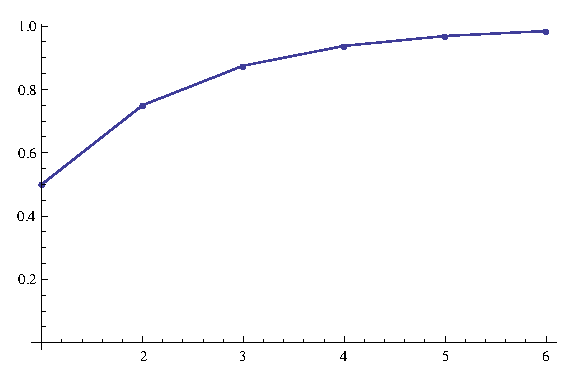
\includegraphics[scale=0.8]{continuous/series/series-3n6n.eps}
        }
        \subfigure[A plot of \( \sum_{n=1}^\infty \frac{2^n}{6^n}. \)]{
          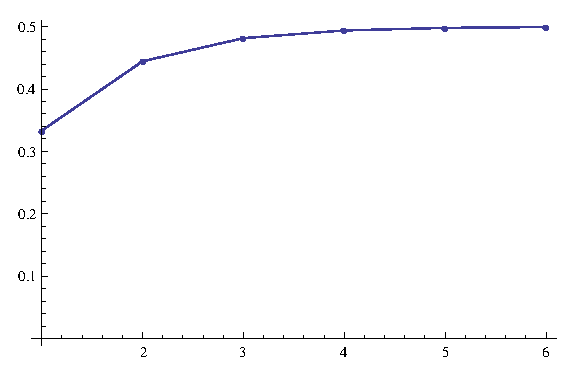
\includegraphics[scale=0.8]{graphs/2pn6pn.eps}
        }
        \subfigure[A plot of \( \sum_{n=1}^\infty \frac{3^n+2^n}{6^n}\).]{
          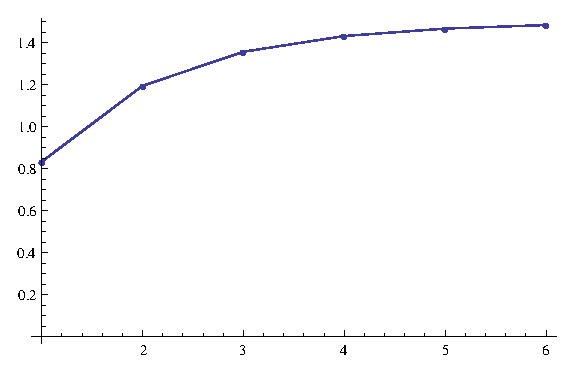
\includegraphics[scale=0.8]{graphs/3pn2pn6pn.eps}
        }
      \end{center}
    \end{figure}

    Finally,
    \begin{align*}
      \sum_{n=1}^{\infty} \frac{3^n+2^n}{6^n}&=\sum_{n=1}^\infty
      \frac{3^n}{6^n} + \sum_{n=1}^\infty
      \frac{2^n}{6^n} \\
      &=1+\frac{1}{2} \\
      &= \frac{3}{2}
    \end{align*}
    \end{sol}
\end{ex}

\section{The Comparison Test}\index{series comparison test}

\begin{theorem}[The Comparison Test]\label{th:seriescomp}
  Let $\sum a_n$, $\sum c_n$, and $\sum d_n$ be series with nonnegative terms.
  Suppose that for some integer $N$
  \[ \forall n > N \bigg(d_n \leq a_n \leq c_n\bigg) \]

  \textbf{(a)} If $\sum c_n$ converges, then $\sum a_n$ also converges.

  \textbf{(b)} If $\sum d_n$ diverges, then $\sum a_n$ also diverges.
\end{theorem}

\section{The Integral Test}\index{series integral test}

Another helpful tool for discovering the behavior of a series is the
\emph{integral test}. In simple terms it is present as follows:
Given the following two statements:
\begin{enumerate}
  \item \(f' < 0 \text{ over } [\ldots, \infty) \)
  \item \(f(n)\) is always positive. We can often see this by writing out some terms.
\end{enumerate}
The integral test states that:

\begin{align*}
  \text{\textbf{(a)}} & \sum^\infty_{n=\ldots} f(n) \text{ converges if }
  \int_{\ldots}^{\infty} f(x) \ud x \text{ converges.}  \\
  \text{\textbf{(b)}} & \sum^\infty_{n=\ldots} f(n) \text{ diverges if } \int_{\ldots}^{\infty} f(x) \ud x \text{ diverges.}
\end{align*}

\begin{proof}
  \begin{align*}
    \int^\infty_1 f(x) \ud x
    &\approx f(1) \Delta x + f(2) \Delta x + f(3) \Delta x + \cdots + \text{with } \Delta x = 1 \\
    &\approx f(1) + f(2)+f(3)+\cdots \\
    &\approx \sum^\infty_{n=1} f(n)\qedhere
  \end{align*}
\end{proof}

\begin{theorem}[The Integral Test]\label{th:seriesint}
  Let $\{a_n\}$ be a sequence of positive terms. Suppose that $a_n = f(n)$,
  where $f$ is a continuous, positive, decreasing function of $x$ for all $x
  \geq N$ ($N \in \mathbb{Z_+}$). Then the series $\sum_{n=N}^\infty a_n$ and
  the integral $\int_N^\infty f(x)\ud x$ both converge or both
  diverge.\cite[p.~554]{thomas}
\end{theorem}

\begin{ex}\label{famousp}
  How do we know that the following series
  \[ \sum^\infty_{n=1} \frac{1}{n} \]
  diverges?
  \begin{sol}
    First, we test it with Theorem \ref{th:nthtermdiv}.
    \[ \lim_{n\to\infty} \frac{1}{n}=0\]
    Because this limit is zero, the test proves inconclusive.

    Let's check the two prerequisites for the integral test. If we let
    $\sum^\infty_{n=1} \frac{1}{n}$ be $\sum^\infty_{n=1}$, and $a_n =
    \frac{1}{n}$, then we can treat $a_n$ as a function and make sure it is
    positive and always decreasing.

    The function \[ f(x)=\frac{1}{x} \]is always positive on $[1, \infty)$.
    Its derivative, \[f'(x)=-\frac{1}{x^2}\] is always negative. Thus, we can
    use the integral test to describe the behavior of $\sum^\infty_{n=1} a_n$.
    \[
      \int^\infty_1 \frac{1}{n} = \lim_{t\to\infty} \ln x |^\infty_1
    \]
    This integral diverges, so by Theorem \ref{th:seriesint} the series also
    diverges.
%%    Note that it it is better to think:
%%    \[ \sum a_n \to \sum^\infty_{n=\ldots} f(n) \]
%%
%%    \[ \sum^\infty_{n=1} \frac{1}{n} \to \int^\infty_1 \frac{1}{x}\ud x \]
%%    \begin{align*}
%%      \int^\infty_1 \frac{1}{x}\ud x
%%      \text{ is }
%%      \int^t_1 \frac{1}{x} \ud x
%%    \end{align*}
  \end{sol}
\end{ex}
\begin{ex}
  Determine whether the following series is convergent or divergent.
  \[ \sum_{k=4}^\infty k e^{-k^2} \]
  \begin{sol}
    We can use the integral test.
    \begin{align*}
      \int_{k=4}^\infty k e^{-k^2} \ud k
      &=\frac{-1}{2}\int_{k=4}^\infty -2 k e^{-k^2} \ud k \\
      &=\frac{-1}{2}e^{-x^2} \bigg|_4^\infty
    \end{align*}
    We can tell that this integral converges, so the series converges.
  \end{sol}
\end{ex}


\section{p Series}

A \(p\) series is of the form.

\[ \sum_{n=1}^{\infty} \frac{1}{n^p} \]

At \(p=1\), it diverges because of the integral test.
This is actually a famous instance of the \(p\)-series.

At \(p=2\), the series converges.

At \(p=-1\), the series diverges.

At \(p=-2\), the series diverges by \ref{th:nthtermdiv}.

At \(p=1.0000000000001\), the series converges by the integral test.

We can get a feeling that \( p>1 \) leads to convergence, and \(p <= 1\) leads to a diverging series.

\begin{homework}
  Online assignment due 04 April 2012 at midnight.

  The next one is due Friday 07 April 2012 at midnight.
\end{homework}

\section{Encyclopedia of Series}

\subsection{Converging series}
\begin{ex}\label{ex:convcomp}
  \[ \sum_{n=1}^{\infty} \frac{5+2\sqrt n}{n^3} \]
  \begin{sol}

    Let $f(x)=\frac{5+2\sqrt{x}}{x^3}$, which is always positive on $x\geq 1$.
    Then $f'(x) = -\frac{5(\sqrt{x}+3)}{x^4}$, which is always negative on $x
    \geq 1$.
    \begin{figure}[h]
      \begin{center}
        \subfigure[A plot of $f(x)=\frac{5+2\sqrt{x}}{x^3}$.]{
          \includegraphics[scale=0.8]{graphs/5p2sqxx3.eps}
        }
        \subfigure[A plot of $f(x)=\frac{5+2\sqrt{x}}{x^3}$.]{
          \includegraphics[scale=0.8]{graphs/n5xp3x4.eps}
        }
      \end{center}
    \end{figure}
    \begin{align*}
      \int_1^\infty \frac{5+2\sqrt x}{x^3} \ud x
      &= \int_1^\infty \frac{5}{x^3} \ud x
      + \int_1^\infty \frac{2 \sqrt x}{x^3} \ud x \\
      &= \int_1^\infty 5x^{-3} \ud x
      + \int_1^\infty 2x^{1/2} \cdot x^{-3} \ud x \\
      &= \lim_{t\to\infty} \int_1^t 5x^{-3} \ud x
      +  \lim_{t\to\infty}\int_1^t 2x^{-5/2} \ud x \\
      &= \lim_{t\to\infty}\frac{5x^{-2}}{-2}\bigg|_1^t+
      \lim_{t\to\infty}\frac{2x^{-3/2}}{-3/2}\bigg|_1^t \\
      &= \lim_{t\to\infty} \bigg[-\frac{5t^{2}}{2}+\frac{4(1)^{-3/2}}{3} \bigg]
      + \lim_{t\to\infty}\bigg[ -\frac{4t^{-5/2}}{3} +\frac{4(1)^{-3/2}}{3}
        \bigg] \\
      &=\lim_{t\to\infty} \bigg[-\frac{5t^{-2}}{2}+\frac{5}{2} \bigg]
      + \lim_{t\to\infty}\bigg[ -\frac{4t^{-3/2}}{3} +\frac{4}{3}
        \bigg]\\
      &=\lim_{t\to\infty} -\frac{5t^{-2}}{2}+\lim_{t\to\infty} \frac{5}{2}
      + \lim_{t\to\infty} -\frac{4t^{-3/2}}{3} +\lim_{t\to\infty}\frac{4}{3} \\
      &=\frac{23}{6}-\lim_{t\to\infty}\bigg[
        \frac{5t^{-2}}{2}+\frac{4t^{-5/2}}{5} \bigg] \\
      &=\frac{23}{6}-\lim_{t\to\infty}\bigg[
        \frac{5}{2t^2}+\frac{4}{3t^{3/2}} \bigg]\\
        &=\frac{23}{6}+0 \\
        &= \frac{23}{6}
    \end{align*}
    By Theorem \ref{th:seriesint}, the series
    \( \sum_{n=1}^{\infty} \frac{5+2\sqrt n}{n^3} \)
    converges.
  \end{sol}
\end{ex}
\begin{ex}
  \[ \sum_{n=1}^{\infty} \frac{5+2\sqrt{n}}{n^3+1} \]
  We can tell that this is quite similar to Example \ref{ex:convcomp}, except we are making the denominator larger.
  We can tell by comparison with the original problem that this must also converge. Likewise, if we made the numerator smaller, we could treat this as converging.
  For a proper solution, we would write
  \begin{sol}
    \[ \sum_{n=1}^{\infty} \frac{5+2\sqrt{n}}{n^3+1} \]
    Converges by comparison with \( \sum_{n=1}^{\infty} \frac{5+2\sqrt n}{n^3} \).
  \end{sol}
  \begin{figure}[h]
    \begin{center}
      \subfigure[A plot of $s_n=\frac{5+2\sqrt{n}}{n^3}$]{
        \includegraphics[scale=0.8]{graphs/5p2sqn3.eps}
      }
      \subfigure[A plot of $s_n=\frac{5+2\sqrt{n}}{n^3+1}$]{
        \includegraphics[scale=0.8]{graphs/5p2sqn3p1.eps}
      }
    \end{center}
  \end{figure}

  Make note, however, that making the denominator smaller does not help us in making these comparisons for convergence.
\end{ex}
\begin{ex}
  \[ \sum_{n=1}^{\infty} \frac{1}{n^4} \]
  This converges.

  \[ \sum_{n=1}^{\infty} \frac{1}{n^4+2} \]
\end{ex}
\begin{ex}
  \[ \sum_{n=1}^{\infty} \frac{2}{n^2+4n+3} \]
  \begin{note}
    We can use partial fraction decomposition to handle this, and it becomes a telescoping sum.
  \end{note}

  \[ \sum_{n=1}^{\infty} \frac{2}{n^2+4n+6} \]
\end{ex}

\begin{remark}
  Imagine we were dealing with one series that conveges to \( \frac{1}{2} \).
  In turn, we were comparing this with another series that ``shoots off into the negatives.''

  We would have issues comparing these in any way.

  Thus, we must check that \(a_n\) and \(b_n\) are exclusively positive.
\end{remark}

\subsection{Diverging Series}
\begin{ex}
  \[ \sum_{n=1}^{\infty} \frac{n}{n+5} \]
  Using theorem \ref{th:nthtermdiv}, we know that this series diverges.

  \[ \sum_{n=1}^{\infty} \frac{n}{n+5-1} \]

  Here, we are decreasing the size of the denominator for a divergent series.
  We can state that \( \sum_{n=1}^{\infty} \frac{n}{n+5-1} \) diverges by comparison with \( \sum_{n=1}^{\infty} \frac{n}{n+5-1} \).
\end{ex}
\begin{ex}
  \[ \sum_{n=1}^{\infty} \frac{(n+1)^2}{n(n+2)} \]
  Diverges by theorem \ref{th:nthtermdiv}.

  \[ \sum_{n=1}^{\infty} \frac{(n+1)^2}{n(n+2)} \]

  Again, making the denominator smaller. This diverges by comparison with the above series.
\end{ex}
\begin{ex}
  \[ \sum_{n=1}^{\infty} \frac{1}{3n+1} \]
  Diverges.
  \[ \sum_{n=1}^{\infty} \frac{15}{3n+1} \]
  Diverges by comparsion with the above.
\end{ex}
\begin{ex}
  \[ \sum_{n=1}^{\infty} \frac{n+2}{n+1} \]
  Diverges.
  \[ \sum_{n=1}^{\infty} \frac{n(n+2)}{n+1} \]
  It doesn't have to be a constant multiple for the comparison test to work.
  We can still state that this diverges by comparison with the above.
\end{ex}


\section{Root Test}\index{series root test}

\begin{theorem}[Root Test]
  Let \(\sum a_n\) be a series with \( a_n \geq 0\) for \(n \geq N\), and
  suppose that
  \[ \lim_{n \to \infty} \sqrt{a_n}^n = \rho \]
  then (a) the series \emph{converges} if \(\rho < 1 \), \textbf{(b)} the series
  diverges if \( \rho > 1\) or if \(\rho\) is infinite, or \textbf{(c)} the test
  is \emph{inconclusive} if \(\rho = 1\).
  \label{th:roottest}
\end{theorem}

\begin{ex}
  Use the root test (txtbk pg. 565) to determine if the following series converges or diverges.
  \[ \sum_{n=1}^\infty \frac{1}{\left( 5n+7 \right)^n} \]
  \begin{sol}
    The root test tells us that
    \[ \rho = \lim_{n \to \infty} \frac{1}{5n+7} \]
  \end{sol}
\end{ex}
\begin{ex}
  \[ \sum_{n=1}^{\infty} \frac{12}{\left( 3+\frac{1}{n}^{4n} \right)} \]
  \begin{sol}
    Use the root test. Take the \(n\)th root of \(s_n\).
    \begin{align*}
      \rho &= \lim_{n \to \infty} \left[ \frac{12}{ \left( 3+\frac{1}{n}^{4n} \right) }\right]^{1/n} \\
      &= \lim_{n \to \infty} \frac{12^{1/n}}{\left( 3+\frac{1}{n} \right)^4}
      \\
      &= \lim_{n \to \infty} \frac{12^{1/n}}{3^4} \\
      &= \frac{1}{81}
    \end{align*}
  \end{sol}
\end{ex}


\section{Ratio Test}\index{series ratio test}

\begin{theorem}[The Ratio Test]\label{th:seriesratio}
  Let $\sum a_n$ be a series with positive terms and suppose that
  \[ \lim_{n \to \infty} \frac{a_{n+1}}{a_n}=\rho \]
  Then \textbf{(a)} the series \emph{converges} if $\rho < 1$, \textbf{(b)} the
  series \emph{diverges} if $\rho > 1$ or $\rho$ is infinite, \textbf{(c)} the
  test is \emph{inconclusive} if $\rho = 1$.
\end{theorem}

\begin{ex}
  Use the ratio test to determine if the following series converges or diverges.
  \[ \sum^\infty_{n=1} \frac{3^n+n}{n!} \]
  \begin{sol}
    First, let's look at the series:
    \[ \frac{4}{1} + \frac{11}{3} + \frac{30}{6} + \cdots \]

    Just use the ratio test, which we can do because this series has exclusively
    positive terms.
    \begin{align*}
      \lim_{n \to \infty}
      \cfrac{\cfrac{3^{n+1}+(n+1)}{(n+1)!}}{\cfrac{3^n+n}{n!}}
      &= \lim_{n \to \infty} \cfrac{(n!)\bigg(3^{n+1}+(n+1)\bigg)}{(3^n+n)(n+1)!} \\
      \intertext{It is important to note here that by factoring a $n+1$ term out
        of $(n+1)!$, we find that $(n+1)! = (n+1)n!$. This
      allows us to manipulate our limit so that some terms will cancel.}
      &= \lim_{n \to \infty}
      \cfrac{(n!)\bigg(3^{n+1}+n+1\bigg)}{(3^n+n)(n+1)(n!)} \\
      &= \lim_{n\to\infty} \frac{3^{n+1}+n+1}{(3^n+n)(n+1)} \\
      &= \lim_{n\to\infty} \frac{3^{n+1}+n+1}{n3^n+n^2+3^n+n} \\
      &= \lim_{n\to\infty}
      \cfrac{\cfrac{3^{n+1}}{3^{n+1}}+\cfrac{n}{3^{n+1}}+\cfrac{1}{3^{n+1}}}
      {\cfrac{n(3^n)}{3^{n+1}}+\cfrac{n^2}{3^{n+1}}+\cfrac{3^n}{3^{n+1}}+\cfrac{n}{3^{n+1}}}
      \intertext{
        Now, as \(n \to \infty\) many of the terms disappear. $n3^n/3^{n+1}$
      becomes $n/3$.}
      &= \lim_{n\to\infty} \cfrac{1}{\frac{n}{3}+\cfrac{1}{3}}\\
      &=\lim_{n \to \infty} \frac{3}{n+1}\\
      &=0
      % &= \lim_{n \to \infty} \frac{3^{n+1}+n+1}{(n+1)(3^n+n)}\\
      % &= \lim_{n \to \infty} \frac{3^{n+1}+n+1}{n3^n+n^2+3^n+n} \\
      % &= \lim_{n \to \infty} \cfrac{3^n \left(
      %  3+\cfrac{n}{3^n}+\cfrac{1}{3^n} \right)}{3^n\left(
      %  n+\cfrac{n^2}{3^n}+1+\cfrac{n}{3^n} \right)} \\
      % &= \lim_{n \to \infty} \cfrac{3+\cfrac{n}{3^n}+\cfrac{1}{3^n}}{n+
      %   \cfrac{n^2}{3^n}+1+\cfrac{n}{3^n}}
    \end{align*}
    Thus, by \ref{th:seriesratio}, this series converges.
    \begin{remark}
      \begin{align*}
        \lim n \to \infty \frac{n}{3^n} \=H \frac{1}{\ln 3 e^{n \ln 3}}
    \end{align*}
    \end{remark}
  \end{sol}
\end{ex}
\begin{ex}
  Use the ratio test to determine if the following series converges or diverges.
  \[ \sum_{n=1}^\infty \frac{n^{19}}{19^n} \]
  \begin{sol}
    Use the ratio test.
    \begin{align*}
      \lim_{n \to \infty}
      \cfrac{\cfrac{(n+1)^{19}}{19^{n+1}}}{\cfrac{n^{19}}{19^n}}
      &= \lim_{n \to \infty} \cfrac{19^n \cdot (n+1)^{19}}{19^{n+1}\cdot n^{19}} \\
      \intertext{$19^n / 19^{n+1}$ becomes just $19$.}
      &= \lim_{n \to \infty} \cfrac{(n+1)^{19}}{19 \cdot n^{19}}
      \intertext{Note that there's no way the \((n+1)^{19}\) and \(n^19\) can in
      any way cancel. However, were we to foil the \((n+1)^{19}\) nineteen
      times, the leading term would be \(n^{19}\). The limit is, therefore, just
    the limit}
    &= \lim_{n \to \infty} \frac{n^{19}}{19n^{19}} \\
    &= \frac{1}{19}
    \end{align*}
  \end{sol}
\end{ex}


\section{Examples}

\begin{ex}
  Does
  \[ \sum_{n=1}^{\infty} \frac{1}{2^n} \]
  converge or diverge?
  \begin{sol}
    \begin{align*}
      s_1 &= \frac{1}{2} \\
      s_2 &= \frac{1}{2} + \frac{1}{4} \\
      s_3 &= \frac{1}{2}+ \frac{1}{4} + \frac{1}{8} \\
      s_4 &= \frac{1}{2}+ \frac{1}{4} + \frac{1}{8} + \frac{1}{16} \\
      s_n &= \frac{2^n-1}{2^n}
    \end{align*}
  \end{sol}
\end{ex}
\begin{ex}
  Does
  \[\sum_{n=2}^{\infty} \frac{n+10}{10n+1} \]
  converge or diverge?
  \begin{align*}
    \lim_{n \to \infty} \frac{n+10}{10n+1} = \\
    \intertext{Divide all terms by \(n\).}
    & \frac{\frac{n}{n}}{\frac{10n}{n}}&=\frac{1}{10} \neq 0 \\
  \end{align*}
  Therefore, the series diverges.
\end{ex}
\begin{ex}
  \[ \sum_{n=0}^\infty \frac{4}{2^n} \]
  \begin{sol}
    Theorem \ref{th:nthtermdiv} gets us nowhere with this one. In other words,
    \[ \lim_{n \to \infty} \frac{4}{2^n} = 0 \]
    is inconclusive.

    We have a geometric series.
    \[ 4 \left( 1+ \frac{1}{2} + \frac{1}{4} + \frac{1}{8} + \frac{1}{16} + \cdots \right) = \frac{1}{1-\frac{1}{2}} \]
    So
    \[ \sum{n=0}^\infty \frac{4}{2^n} \]
    converges to \(8\).
  \end{sol}
\end{ex}
\begin{ex}
  Does
  \[ \sum_{n=1}^\infty \frac{1}{n}-\frac{1}{n-2} \]
  converge or diverge?
  \begin{sol}
    Check the limit.
    \begin{align*}
      \lim_{n \to \infty} \frac{1}{n} - \frac{1}{n-2} &=
      \lim_{n \to \infty} \frac{n-2}{n(n-2)} - \frac{n}{n(n-2)} \\
    \end{align*}
    \[
      \frac{1}{1}-\frac{1}{3}+\frac{1}{2}-\frac{1}{4}+\frac{1}{3}-\frac{1}{5}+\cdots
    \]
    This is called a telescoping sum that converges to \(\frac{3}{2}\).
  \end{sol}
\end{ex}
\begin{ex}
  \[ \sum_{n=1}^{\infty} \frac{n+1}{2n-1} \]
  \begin{sol}
    Check the limit.
    \[ \lim_{n \to \infty} \frac{n+1}{2n-1}\neq0 \]
    The series diverges.
  \end{sol}
\end{ex}
\begin{ex}
  \[ \sum_{n=1}^{\infty} \frac{3n-1}{2n+1} \]
  Check the limit.
    \[ \lim_{n \to \infty}\frac{3n-1}{2n+1}\neq0 \]
    The series diverges.
\end{ex}
\begin{ex}
  \[ \sum_{n=0}^{\infty} \frac{1}{4^n} \]
  \begin{sol}
    \[ \frac{1}{1}+\frac{1}{4}+\frac{1}{16}+\frac{1}{32}+\ldots \]
    Converges to \(\frac{1}{1-\frac{1}{4}}\).
  \end{sol}
\end{ex}
\begin{ex}
  \[ \sum_{n=0}^{\infty} (1.075)^n \]
  \begin{sol}
    $\lim_{n\to\infty} (1.075)^n\neq0$ and the series diverges because of
    Theorem \ref{th:nthtermdiv}.
  \end{sol}
\end{ex}
\begin{ex}
  \[ \sum_{n=1}^\infty \frac{2^n}{100} \]
  \begin{sol}
    $\lim_{n\to\infty} \frac{2^n}{100}\neq 0$ so by Theorem \ref{th:nthtermdiv}
    the series diverges.
  \end{sol}
\end{ex}
\begin{ex}
  \[ \sum_{n=1}^\infty \frac{2^n}{n^2} \]
  \begin{sol}
    \(2^n\) is geometric but the \(n^2\) denominator means we can't treat it
    like a geometric series.

    Using Theorem \ref{th:nthtermdiv}, we find that
    \begin{align*}
      \lim_{n\to\infty} \frac{2^n}{n^2}&=\lim_{n\to\infty} \frac{e^{n\ln2}}{n^2}
      \\
      &\=H \lim_{n\to\infty} \frac{\ln 2 e^{n \ln 2}}{2n} \\
      &\=H \lim_{n\to\infty} \frac{2\ln 2 e^{n \ln 2}}{2} \\
      &\neq 0
    \end{align*}
    so the series diverges.
  \end{sol}
\end{ex}
\begin{ex}
  \[ \sum_{n=1}^\infty \frac{1}{n(n+3)} \]
  \begin{sol}
    Checking with \ref{th:nthtermdiv} proves inconclusive.

    We can use partial fraction decomposition on this fraction.
    \begin{align*}
      \frac{1}{n(n+3)} =& \frac{A}{x}+\frac{B}{x+3} \\
      \intertext{We find that \( A = \frac{1}{3} \) and \(B = -\frac{1}{3} \)}
      =& \frac{1/3}{x}-\frac{1/3}{x+3}
    \end{align*}

    \begin{align*}
      \sum_{n=1}^\infty \frac{1}{n(n+3)} =& \frac{1}{3} \sum_{n=1}^\infty \left(\frac{1}{n}-\frac{1}{n+3}\right)
    \end{align*}
  \end{sol}
\end{ex}
\begin{ex}
  \[ \sum^\infty_{n=4} \frac{1}{(n-3)^2} \]
  \begin{sol}
    Check it with Theorem \ref{th:nthtermdiv}:
    \[ \lim_{n \to \infty} \frac{1}{(n-3)^2} = 0 \]
    Which is inconclusive, so we will attempt to use the integral test.
    \[ f(x) = \frac{1}{(x-3)^2} \]
    Check the derivative:
    \begin{align*}
      f'(x) &= \frac{(x-3)^2 \frac{\ud}{\ud x}(1) - 1 \frac{\ud}{\ud x}(x-3)^2} {(x-3)^4} \\
        &= \frac{-2(x-3)}{(x-3)^4} \\
        &= \underbrace{\frac{-2}{(x-3)^3}}_{\text{DNE when } x=3 }
    \end{align*}
    \begin{table}[h]
      \centering
      \boxed{
        \begin{tabular}{r|c|c|c}
          $x$ & $-\infty$ & $3$ & $\infty$ \\ \hline
          $f(x)$ & \multicolumn{3}{c}{$+$} \\ \hline
          $f'(x)$ & $-$ & \text{ undefined } & $-$
        \end{tabular}
      }
      \caption{A sign diagram of $f(x)$ and $f'(x)$}
    \end{table}
    $f(x)$ is always positive, and $f'(x)$ is always negative, so the first two prerequisites for theorem \ref{th:seriesint} are passed.

    Now consider
      \[ \int^\infty_4 \frac{1}{(x-3)^2} \ud x  \]
    {First evaluate this as an indefinite integral:}
    \begin{align*}
      \int \frac{1}{(x-3)^2}\ud x
      &=\int \frac{1}{u^2}\ud u =\int u^{-2} \ud u \\
      &=\frac{u^{-1}}{-1} \\
      &=\frac{-1}{(x-1)}
    \end{align*}
      {Now evaluate it in terms of the original definite integral:}
    \begin{align*}
      \int^\infty_4 \frac{1}{(x-3)^2} \ud x
      &=\lim_{t\to\infty} \frac{-1}{(x-1)}\bigg|^t_4 \\
      &=-\lim_{t\to\infty} \frac{1}{(t-1)}+\frac{1}{3} \\
      &=-\frac{1}{3}
    \end{align*}
    This integral converges, so the $\sum^\infty_{n=4}
    \frac{1}{(n-3)^2}$ must converge (though we don't know to what).
  \end{sol}
\end{ex}
\begin{homework}
  \date{30 March 2012}

  Read Section 10.4

  pg. 562 \# 1, 3, 5, 6 (converges by comparison with \(\frac{1}{3^n}\), 7, 33, 35, 37, 41, 47
\end{homework}
\begin{ex}
  Does the following series converge or diverge?
  \[ \sum_{n=1}^\infty \frac{\ln n}{n} \]
  \begin{sol}
    Check Theorem \ref{th:nthtermdiv} first and foremost.
    \begin{align*}
      \lim_{n \to \infty} \frac{\ln n}{n}
      &\=H \lim_{n \to \infty} \frac{\frac{1}{n}}{1} \\
      &= 0
    \end{align*}

    Next, check with the integral test, theorem \ref{th:seriesint}.

    We know that the \(\ln x\) is positive past \(x=1\), so the second condition
    for use of the theorem is satisfied.

    The first condition is slightly more difficult:

    \begin{align*}
      f' &= \frac{x \cdot \frac{1}{x}- \ln x}{x^2} \\
      &= \frac{1- \ln x}{x^2}
    \end{align*}

    Which is \( > 0 \), so we can use the integral test.

    \begin{align*}
      \int_{1}^{\infty} \frac{\ln n}{n} \ud x \\
      \frac{(\ln x)^2}{2} \bigg|_{1}^{\infty}
    \end{align*}

    We can conclude that the series diverges.
  \end{sol}
\end{ex}
\begin{ex}
  Does the following series converge or diverge?
  \[ \sum^\infty_{n=1} \frac{3}{\sqrt{n}} \]
  \begin{sol}
    Recognize this as a \(p\)-series with \(p=1/2\).

    Note that, without the \(3\), we would be looking at a definitely diverging
    \(p\)-series.

    However, multiply that diverging series by \(3\) and we are dealing with an
    even \emph{bigger} diverging \(p\)-series.

    The series, therefore, diverges by comparison with \[
      \sum_{n=1}^\infty \frac{1}{\sqrt{n}} \]
  \end{sol}
\end{ex}
\begin{ex}
  Determine if this geometric series converges or diverges. If it converges,
  find its sum.
  \[ (1/5) + (1/5)^2 + (1/5)^3 + (1/5)^4 + \cdots \]
  \begin{sol}
    Treat it as a geometric series and multiply it as such.
    \[ \left( 1-\frac{1}{5} \right) \left(\frac{1}{5} + (1/5)^2 + (1/5)^3 + (1/5)^4 +
      \cdots \right) = \frac{1}{5} \]
    So now we look for our final answer:
    \begin{align*}
      \frac{\frac{1}{5}}{1-\frac{1}{5}} = \frac{1}{4}
    \end{align*}
  \end{sol}
\end{ex}
\begin{ex}
  If the series \[ \sum^{\infty}_{n=0} \cos{9n\pi} \] converges, then what is
  its sum.
  \begin{sol}
    This turns out to just be a fancy way of writing
    \[ \sum 1-1+1-1+1-1+1-1+\cdots \]

    Alternatively, we are talking about a cosine function. The cosine function
    never settles down, it constantly jumps back and forth between values. Thus,
    we could take the limit as \( n \to \infty\) of \(s_n\) to find that it
    diverges.
  \end{sol}
\end{ex}
\begin{ex}
  Find a formula for the \(n\)th partial sum of the series and use it to
  determine if the series converges.
  \[ \sum_{n=1}^\infty (\ln \sqrt{n+1} - \ln \sqrt{n}) \]
  \begin{sol}
    \begin{align*}
      s_1 &= \ln \sqrt{2} - \ln \sqrt 1 \\
      s_2 &= \ln \sqrt 3 - \ln \sqrt 2 + \ln \sqrt 2 - \ln \sqrt 1 \\
      s_3 &= \ln \sqrt 4 - \ln \sqrt 3 + \ln \sqrt 3 + \ln \sqrt 2 - \ln \sqrt 1
      \\
      s_4 &= \ln \sqrt 5 - \ln \sqrt 4 + \ln \sqrt 4 - \ln \sqrt 3 + \ln \sqrt 3
      - \ln \sqrt 2 + \ln \sqrt 2 - \ln \sqrt 1 \\
      s_5 &= \ln \sqrt 6 - \ln \sqrt 5 + s_4 \\
      s_n &= \ln \sqrt{n+1}-\ln \sqrt{1}
    \end{align*}
    \[ \sum^\infty_{n=1} \text{ is } s_\infty \]
    We can conclude that the series diverges.
  \end{sol}
\end{ex}
\begin{ex}
  Use the limit comparison test to determine convergence or divergence.
  \[ \sum^\infty_{n=1} \frac{n}{n^2 + 7n +5} \]
  \begin{sol}
    \begin{align*}
      \lim_{n \to \infty} \frac{\frac{n}{n^2+7n+5}}{\frac{1}{n}} =1
    \end{align*}
    This is about the same order of magnitude as our original problem. The
    numerator and the denominator balance, and the limit takes us to 1, so the
    series diverges.
  \end{sol}
\end{ex}
\begin{ex}
  Tell whether the series converges or diverges. If it converges, give its sum.
  \[ 1 + \frac{8}{9} + \left( \frac{8}{9} \right)^2 + \left(
    \frac{8}{9} \right)^3+ \cdots + \left( \frac{8}{9} \right)^n + \cdots \]
  \begin{sol}
    Treat this as a geometric series.

    We will find the answer converges to $9$.
  \end{sol}
\end{ex}
\begin{ex}
  Does the series
  \[ \sum^\infty_{n=1} \frac{5}{n^2+36} \]
  converge or diverge? If so, to what?
\end{ex}
\begin{ex}
  If the series \[ \sum_{n=0}^\infty \left( \frac{3}{\sqrt{13}} \right)^n \]
  converges, what is its sum?
  \begin{sol}
    \[\left( 1-\frac{3}{\sqrt{13}} \right) \left[ 1+\frac{3}{\sqrt{13}}+\left( \frac{3}{\sqrt{13}} \right)^2+\ldots \right] \]
  \end{sol}
\end{ex}
\begin{ex}
  Find a formula for the \(n\)th partial sum of the series.
  \[ \sum^\infty_{n=1} \left( \frac{1}{n}-\frac{1}{n+1} \right) \]
  \begin{sol}
    \[ s_n = 1-\frac{1}{n+1} \]
  \end{sol}
\end{ex}
\begin{ex}
  Does the series
  \[ \sum^\infty_{n=1} \frac{4e^n}{1+e^{2n}} \]
  converge or diverge?
  \begin{sol}
    This series is a variation of
    \begin{align*}
      \sum^\infty_{n=1} \frac{4e^n}{e^{2n}} &=
      4 \sum^\infty_{n=1} \frac{e^n}{e^{2n}} \\
      &= 4 \sum^\infty_{n=1} \left( \frac{1}{e} \right)^n
    \end{align*}
    Which is a geometric series.

    The original series converges by comparison with the above.
  \end{sol}
\end{ex}
\begin{ex}
  Use the limit comparison test to determine if the following series converges
  or diverges by comparison with \(\sum^\infty_{n=2} \frac{1}{n} \).
  \[ \sum^\infty_{n=2} \frac{1}{\ln n} \]
  \begin{sol}
    Remember that the limit comparison test is far different from the comparison
    test.
    \begin{align*}
      \lim_{n \to \infty} \frac{\frac{1}{\ln n}}{\frac{1}{n}} &=
      \lim_{n \to \infty} \frac{n}{\ln n} \\
      \=H \lim_{n \to \infty} \frac{1}{\frac{1}{n}} \\
      &= \lim_{n \to \infty} n
    \end{align*}
    \(n\) diverges as it goes toward \(\infty\).
  \end{sol}
\end{ex}

\section{Alternating Series Test}

\begin{theorem}[Leibniz's Test]\index{Leibniz's Test}\index{alternating series
  test}\label{th:alternatingseries}\cite[p.~568]{thomas}
  The series
  \[ \sum^\infty_{n=1} (-1)^{n+1} u_n = u_1 - u_2 + u_3 - u_4 + \cdots \]
  converges if all three of the following conditions are satisfied:
  \begin{enumerate}
    \item The $u_n$'s are all positive.
    \item The postive $u_n$'s are (eventually) noincreasing: $u_n \leq u_{n+1}
      for all n \geq N$, for some integer $N$.
    \item $u_n \to 0$
  \end{enumerate}
  \begin{note}
    Also known as the alternating series test.
  \end{note}
\end{theorem}
\begin{proof}
  Let's write out some of the terms of an alternating series, see how it's
  playing out:
  \[ u_1 - u_2 + u_3 - u_4 + \cdots\]
  \begin{remark}
    These could start negative, too, and we would just factor that out of the sum
    to make it postive and fit the theorem.
  \end{remark}
  \begin{align*}
    s_2 &= u_1 - u_2 \geq 0 \\
    s_4 &= s_2 + (u_3 - u_4) \geq s_2 \\
    s_6 &= s_4 + (u_5 - u_6) \geq s_4
  \end{align*}
  So we see, at each step, that the sequence of partial sums is monotonic
  increasing. To know that it converges, we mus first show that it is bounded.

  The sequence of partial sums gets larger and larger so the lower bound is
  \[ s_n = u_1 - \overbrace{(u_2 - u_3)}^+ - \overbrace{(u_4 - u_5)}^+ \]
  The \emph{sequence of partial sums} is monotonic and bounded by $M=u$ and
  $m=s_2$.

  Therefore, the series converges.
\end{proof}
\begin{ex}
  \[ \sum^\infty_{n=1} (-1)^n \frac{3n}{4n-1} \]

  Although at first this appers to be an alternating series, it actually
  diverges by Theorem \ref{th:nthtermdiv}, the limit test.
\end{ex}
\begin{ex}
  \[ \sum^\infty_{n=1} (-1)^{n+1} \left( \frac{3n+2}{4n^2+3} \right) \]
  \begin{sol}
    Check with \ref{th:nthtermdiv}, which proves inconclusive.

    Take the derivative of $f(x)=(-1)^n \frac{3n}{4n-1}$. We find $f'(x)$ is
    negative everywhere.
    \begin{align*}
      f'(x)&=12x^2-9-24x^2-16x \\
      f'(x)&=-12x^2-16x-9
    \end{align*}
    By Theorem \ref{th:alternatingseries}, this series converges.
  \end{sol}
\end{ex}

So far, we've been able to tell to what number very few infinite sums converge.
Geometric and telescoping sums, for example. For convergent alternating series,
we can always estimate the limit, $L$, and measure the error of our estimation,
the discrepancy between this estimate and the actual theoretical value of
$L$.\footnote{There's an awesome diagram about this in the textbook. Check out
  \cite[p.~569 Fig.~10.13]{thomas}.}

This error is given by
\begin{equation}
  \pm | L - S_n |
\end{equation}

\begin{homework}
  Read section 10.8

  pg 588 odd 1-9, 11, 13, 23, 25, 27
\end{homework}

\section{Power Series}\index{Power Series}[Thomas' Calculus pg 575]
A \textbf{power series} about $x=0$ is the form
\[ \sum_{n=0}^\infty c_n x^n = c_0 + c_1 x + c_2 x + \cdots. + c_n x^n + \cdots
  \]
  And a power series about $x=a$ is of the form
  \begin{equation}\label{eq:powerxa} \sum_{n=0}^\infty c_n (x-a)^n = c_0 + c_1 (x-a) + c_2 (x-a)^2 +
    \cdots + c_n (x-a)^n + \cdots \end{equation}
    in which the center $a$ and the coefficicents $c_0, c1, c2, \cdots$ are
    constants.

    Taking all the coefficients to be $1$ in equation \eqref{eq:powerxa}
    gives us the \textbf{geometric series}\index{geometric series}
    \begin{equation}\label{eq:geopower}
      \szinfty x^n = 1 + x + x^2 + x^3 + x^4 + x^5 + \cdots + x^n  + \cdots
    \end{equation}
    \begin{figure}[h]
      \begin{center}
        \includegraphics{continuous/series/geopower.eps}
      \end{center}
      \caption{A plot of equation \eqref{eq:geopower}.\label{fig:geopower}}
    \end{figure}
    This is the geometric series with the first term $1$ and the ratio $x$.
    It converges to $1/(1-x)$ for $|x|<1.$ As shown in Figure
    \ref{fig:geopower}, the series has a vertical asymtote at $x=1$ and we
    cannot approximate it at $x \geq 1$.
    \begin{theorem}
      [Reciprocal Power Series]\index{reciprocal power
      series}\label{th:recipowser}
      \begin{equation}
        \frac{1}{1-x} = \sum_{n=0}^{\infty}x^n, \quad |x| < 1
      \end{equation}
    \end{theorem}
\begin{ex}
  \[ \sum^\infty_{n=0} n^3 x^n   \]
  An example of a \textbf{power series}, where the coefficient depends on where
  you are adding the polynomial.\label{powerseriesex1}
  Otherwise described as a \emph{power series about \(x=0\)}.
\end{ex}
\begin{ex}
  \[\sum^\infty_{n=0} n^3 (x-5)^n\]
  This is nothing more than example \ref{powerseriesex1} shifted 5 to the right.
  Otherwise described as a \emph{power series about \(x=5\)}.
  \begin{sol}
    Ratio test.
    \begin{align*}
      \lim{n\to\infty} \bigg| \frac{(n+1)^3 (x-5^{n+1}}{n^3 (x-5)^n} \bigg|
      &=
      \lim{n\to\infty} \bigg| \frac{(n+1)^3 (x-5^{1}}{n^3} \bigg| \\
      \intertext{Factor out the polynomial and take the limit by dividing each
      term by the highest power.}
      &= | x-5| \cdot \lim_{n\to \infty} \frac{n^3+3n^2+3n+1}{n^3} \\
      &= |x-5| \cdot 1 \\
      &= |x-5|
    \end{align*}
    \[ |x-5| < 1 \]
    This has an interval of convergence from $4$ to $6$.
    \begin{note}
      For this to be correct, we \textbf{must} consider:
      \[ \sum^\infty_{n=0} n^3 (6-5)^n \]
      This one diverges by the \emph{nth term test}.
      \[ \sum^\infty_{n=0} n^3 (4-5)^n \]
      because the ratio test is inconclusive at $x=1$.
      Although this is an alternating series, this one diverges by the \emph{nth
      term test}.

      The interval $(4, 6)$ is the interval of convergence. This interval is
      \emph{about} $x \approx 5$.

      This is sometimes called a ``radius of convergence\index{radius of
      convergence},'' drawn as a circle on
      a number line.
    \end{note}
  \end{sol}
\end{ex}
We want to talk about what kind of $x$ values will result in a finite sum, or
infinite sum.
\begin{note}
  An interval of convergence can be $-\infty<x<\infty$. The radius of
  convergence would thus be $\infty$.
\end{note}
\begin{ex}
  An interval of convergence from $3 < x < 7$. The radius of convergence is $2$.
\end{ex}

\section{Taylor and Maclauren Series}

This is used to approximate ``ugly'' functions with polynomial(s). In the
business world, this is useful such that we are not working with increasingly
complicated functions.

\begin{ex}
  \[ f(x) =  e^x \]
  \begin{figure}[h]
    \begin{center}
      \includegraphics{continuous/series/etx.eps}
    \end{center}
    \caption{A plot of $f(x)=e^x$.}
    \label{fig:etx}
  \end{figure}
  Before we start, we must decide \emph{where} we are going to make the
  approximation.

  Say we are attempting this at $x=1$, for example. So the function is constant.

  \[ f(x) = A \]
  \begin{figure}[h]
    \begin{center}
      \includegraphics{continuous/series/etx2.eps}
    \end{center}
    \caption{A plot of $e^x$ and $e$.}
    \label{fig:etx2}
  \end{figure}
  The best approximation is $f(x)=e^1$. This intersects the graph of $f(x)=e^x$
  at $x=1$. This is called at \textbf{$0$th order approximation}.

  This can get the slope right at one point.

  \[ f(x)=c_0 + c_1x\]
  [ include a plot ]
  Treat this function as a y value. The $y$ values is $e^1$.
  \[e^1=c_0+c_1 \cdot 1\]
  We have one equation and two unknowns. We should also, here, approximate the
  slope of $e^x$ at $x=1$.
   \begin{align*}
    e^1&=c_0+c_1 \cdot 1 \\
    (e^x)' \bigg|_{x=1} &\equiv c_1
  \end{align*}
  To solve this, recognize $c_1$ is $e^1$. Plug this into the first equation for
  your coefficients.

  \[ f(x) = c_0 + c_1x + c_2x^2 \]
  [plot]
  This will hopefully get the concavity right.
  \[e^1= c_0+c_1(1)+c_2(1) \]
  \begin{align*}
    e^1&=c_0+c_1 \cdot 1 \\
    (e^x)' \bigg|_{x=1} &\equiv c_1 + 2 c_2 \\ \intertext{take the second
    derivative for concavity.}
    (e^x)'' \bigg|_{x=1} &\equiv 2 \cdot 1 \cdot c_2 \\
  \end{align*}
  Now, starting with finding $c_2$, we can get the coefficients for all the
  preceding equations.

  \[ f(x) = c_0 + c_1x + c_2x^2+c_3x^3 \]
  [plot]
  We are doing a better job of approximating $e^x$ at each step. Now we will put
  a cubic function as our approximation.
  \begin{align*}
    e^1&=c_0+c_1 \cdot 1+c_2 \cdot 1^2 + c_3 \cdot 1^3 \cdot 1 \\
    (e^1)' \bigg|_{x=1}&=+c_1 +2c_2 \cdot x \bigg|_{x=1}  +3 c_3 \cdot
    x^2\bigg|_{x=1} \cdot 1 \\ \intertext{Here we get the slope to be correct.}
    (e^x)'' \bigg|_{x=1} &= 2 c_2 + c_3 \cdot x^2 \bigg|_{x=1} \\
    (e^x)''' \bigg|_{x=1} &= 3 \cdot 2 \cdot 1 \cdot c_3
  \end{align*}

  We notice that \[\frac{ (e^x)^n \bigg|_{x=1}}{n!} = c_n \]

  Ths is what we call a \emph{Taylor series approximation} of $f(x)$ at $x=1$.
\end{ex}

\begin{theorem}
  The \textbf{Taylor series} approximation of $f(x)$ at $x=a$ is
  \[ f \bigg|_{x=a} + f'\bigg|_{x=a} + \frac{f''\bigg|x=a}{2!} \cdot (x-a)^2 +
    \frac{f'''\bigg|_{x=a} (x-a)^3}{3!} + \frac{f''''\bigg|_{x=a} (x-a)^4}{4!} +
    \cdots\]
  \label{th:taylorseries}
\end{theorem}
\begin{ex}
  Find a Taylor series apprximation of
  \[ f(x) = \ln x \]
  at $x=2$.
  \begin{sol}
    \[ \ln 2 + \frac{1}{x} \bigg|_2 (x-2) + \frac{-1}{x^2} \bigg|_2
      \frac{(x-2)^2}{2!} + \frac{2}{x^3}\bigg|_{x=2} \frac{(x-2)^3}{3!}
      + \frac{-6}{x^4}\bigg|_{x=2} \frac{(x-2)^4}{4!} + \cdots\]
      Taylor series are power series. This yields a \emph{power series} about
      $x=2$.
  \end{sol}
\end{ex}
\begin{ex}
  Find a Taylor series of
  \[ f(x) = \sin x \]
  at $x=0$.
  \begin{sol}
    We see odd numbers appear.
    \begin{align*}
      \sin x &\approx \left[ \sin 0 + \cos x (x-0)^1 + \frac{-\sin x (x-0)^2}{2!} -
      \cos x (x-0)^{3}{3!} + \frac{\sin x (x-0)^4}{4!} \right]_{x=0} + \frac{\cos x
      (x-0)^5}{5!}
      \cdots
      \\
      \sin x &\approx 0+x - \frac{x^3}{3!} + \frac{x^5}{5!} + \cdots
  \end{align*}
  We could, in other words, write this as
  \[ \sin x = \sum_{n=0}^\infty \frac{(-1)^n \cdot x^{2n+1}}{(2n+1)!} \]
  This is a \emph{power series about} $x=0$.
  Since we have a power series, we can find its \emph{interval of convergence.}

  \[ \lim_{n\to\infty} \frac{(-1)^{n+1} x^{2(n+1)+1}}{[2(n+1)+1]!} \]
  An $x^2$ factors.
 We're left with   \[ \lim_{n\to\infty} \frac{(-1)^{n+1}
   x^{2(n+1)+1}}{[2(n+1)+1][2(n+1]} \]
  The interval of convergence is $-\infty<x<\infty$.
  \end{sol}
\end{ex}

\chapter{Complex Numbers}\label{ch:complex}
Earl A. Coddington, professor of mathematics at UCLA, offers an extremely helpful crash-course in complex numbers in his book \emph{An Introduction To Ordinary Differential Equations}, Chapter 0 \cite{coddington}.
Most of the initial knowledge in this chapter comes from my notes on that chapter, but I will attempt to provide pictures and examples where I found the source text lacking.
\begin{defn}
  A \keyword{complex number}{complex number} is an ordered pair of real numbers $(x, y)$.
  If $z$ is a complex number, we write
  \begin{equation}
    z = (x,y).
  \end{equation}
\end{defn}
\begin{defn}
  The \keyword{sum}{complex sum} $z_1+z_2$ is the complex number given by
  \begin{equation}
    z_1 + z_2 = (x_1 + x_2, y_1 + y_2).
    \label{eq:complexsum}
  \end{equation}
\end{defn}
\begin{defn}
  If $z=(x,y)$, the \keyword{negative}{negative} of $z$, denoted $-z$, is defined to be the number
  \begin{equation}
    -z = (-x, -y).
  \end{equation}
\end{defn}
\begin{defn}
  The \keyword{zero}{zero} complex number, written simply 0, is defined as
  \begin{equation}
    0 = (0, 0).
  \end{equation}
\end{defn}
Since \eref{eq:complexsum} defines complex sums in terms of just real number addition operations, and we know that these real number operations are commutative, it follows that
\begin{equation}
  z_1+z_2 = z_2 + z_1.
\end{equation}
Likewise does the associative property of addition for real numbers hold for complex numbers:
\begin{equation}
  (z_1 + z_2) + z_2 = z_1 + (z_2 + z_3).
\end{equation}
And the number $0$ provides our additive identity:
\begin{equation}
  z + 0 = z.
\end{equation}
Finally, we have an additive inverse for complex numbers
\begin{equation}
  z+(-z)=0.
\end{equation}
For additional information on these properties as they apply to the set of real numbers, I will direct the reader to Michael Spivak's \emph{Calculus, Third Edition}, perhaps the single greatest introduction to ``real mathematics'' ever written.
These properties, and their importance with regard to real numbers, is detailed extensively in the first chapter.
\begin{defn}
  The \keyword{difference}{difference}, $z_1-z_2$, is defined by
  \begin{equation}
    z_1-z_2 = z_1 + (-z_2).
  \end{equation}
\end{defn}
\begin{defn}
  The \keyword{product}{product} $z_1z_2$ is defined by
  \begin{equation}
    z_1z_2 = (x_1x_2 - y_1y_2, x_1 y_2 + x_2 y_1).
    \label{eq:complex_product}
  \end{equation}
\end{defn}
\begin{remark}
  \eref{eq:complex_product} can be found by performing basic multiplication on the following form of the numbers:
  \begin{align*}
    z_1 &= x_1 + \iu y_1 \\
    z_2 &= x_2 + \iu y_2 \\
    z_1z_2 &= (x_1+\iu y_1)(x_2 + \iu y_2)
  \end{align*}
  In order to use this, however, we must define the following units:
\end{remark}
\begin{defn}
  The \keyword{unit}{unit} complex number is the number $(1,0)$.
  This may be multiplied by any complex number $z=(x,y)$ and the product will always be $z$.
\end{defn}
\begin{defn}
  The \keyword{imaginary unit}{imaginary unit} is defined to be the number \[\iu = (0,1).\]
\end{defn}
From those definitions, we see that if $z=(x,y)$ we can write it in terms of its real and imaginary parts as follows:
\begin{align}
  z&=x(1,0)+y(0,1),
  \intertext{which is equivalent to stating}
  z&=x+\iu y.
\end{align}


\chapter{Ordinary Differential Equations}
\begin{defn}
  A \textbf{differential equation} is an equation involving derivatives.
\end{defn}
\begin{defn}
  A \textbf{direction field} tells us the slope of a function at any given place.
\end{defn}
\begin{ex}
    In physics, we often define acceleration to be a vector relative to another 
    vector, velocity.
    Here, we will just consider them as scalars for the sake of argument.
    Accleration is a change in velocity, so
    \begin{equation}
        a = \leib{v}{t},
        \label{eq:acceleration}
    \end{equation}
    where $v$ represents velocity and $t$ represents time.
    Now we integrate both sides of \eref{eq:acceleration} with respect to $t$,
    \begin{equation}
        \int a \ud t = \int \leib{v}{t} \ud t.
        \label{eq:intaccel}
    \end{equation}
    Now, assuming\footnote{This must be explained later, but as a warning: no,
    the $\ud t$ in the derivative operation and the $\ud t$ in the integration 
    operation do not simply cancel.}
    \begin{equation}
        \int \leib{v}{t} \ud t = \int \ud v,
        \label{eq:handwave}
    \end{equation}
    then using \eref{eq:handwave}, we see that
    \begin{equation}
        \int a \ud t = \int \ud v.
        \label{eq:naughtint}
    \end{equation}
    From here we simplify, finding that
    \begin{equation}
        at + c_1 = v + c_2.
        \label{eq:almostvelocity}
    \end{equation}
    The constants in \eref{eq:almostvelocity} are simply constants and may be combined into another constant, $C$.
    Also, the equation may be rearranged to put it in more familiar form, yielding
    \begin{equation}
        v = at + C,
        \label{eq:velocity}
    \end{equation}
    which we recognize as the classical mechanics equation for velocity.
    Integrating once more, and replacing $v$ with the definition of velocity as change in position, we find
    \begin{align}
        \int \leib{x}{t} \ud t &= \int (at + C) \ud t, \nonumber \\
        \int \leib{x}{t} \ud t &= \int at \ud t + \int C \ud t, \nonumber \\
        x + c_3  &= a \frac{t^2}{2} + Ct + c_4. \nonumber \\
        \intertext{Now we may simply combine the constants once more, defining $C_1$ to constitute the difference of $c_4$, and $c_3$,}
        x &= a \frac{t^2}{2} + Ct + C_1. \label{eq:phys_const}
    \end{align}
    \eref{eq:phys_const} may be rewritten in its more common form:
    \begin{equation}
        x(t) = \frac{1}{2} a t^2 + v_0 t + x_0.
        \label{eq:position}
    \end{equation}
\end{ex}

% \section{Integrating Factors}
% We will observe differential equations of the form
% \begin{equation}
%   \leib{y}{t} = g(t) y + r(t)
% \end{equation}
% \begin{enumerate}
%   \item $\leib{y}{t} = t^2 y + \cos{t}$
%   \item $t y +3=\leib{y}{t}-2t$
% \end{enumerate}

